\documentclass[landscape]{progbookcn}
\usepackage{lmodern}
\usepackage{multicol}
\usepackage[ruled, lined, linesnumbered, commentsnumbered, noend]{algorithm2e}
\usepackage{algpseudocode}
\usepackage{amsmath}
\usepackage{amsthm}
\usepackage{amssymb}

\newcommand{\bigo}[1]{$\mathcal{O}$(#1)}

\DeclareMathSymbol{\mlq}{\mathord}{operators}{``}
\DeclareMathSymbol{\mrq}{\mathord}{operators}{`'}

\begin{document}

%% title page
    \begin{titlepage}
    \vspace*{25ex}
  
    \hspace{0.05\textwidth}\begin{minipage}{.9\textwidth}
      \flushright
  
      %%中文书名
      {\zihao{1}\textbf{算法学习:AcWing}}
  
      \rule{\linewidth}{.5pt}
  
      \vspace{2ex}
  
      %% 英文书名
      {\zihao{2}\textsf{Algorithm Learning: AcWing}} \\
  
      \vspace{20ex}
  
      %% 作者
      {\zihao{4}\textit{吴小强}~编著}
    \end{minipage}
  
    \vfill
  
    \centering
    {\zihao{4}深圳 ~$\bullet$ ~SHENZHEN}
  \end{titlepage}
    \thispagestyle{empty}

    \frontmatter

    \chapter{前言}

% 本书是在 \href{https://www.acwing.com/}{AcWing} 学习的记录,序言留待后续补足。

%% 目录
    \clearpage
    {
        \hypersetup{hidelinks}
        \tableofcontents
    }

    \mainmatter


    \part{算法基础}
    \label{alg_foundation_part}
    \chapter{算法基础}


\section{快速排序}

\subsection{AcWing 785. 快速排序}

\begin{titledbox}{AcWing 785. 快速排序}
    给定你一个长度为 $n$ 的整数数列。请你使用快速排序对这个数列按照从小到大进行排序。并将排好序的数列按顺序输出。

    输入格式:

    输入共两行,第一行包含整数 $n$。第二行包含 $n$ 个整数(所有整数均在 $1 \sim 10^9$ 范围内),表示整个数列。

    输出格式:

    输出共一行,包含 $n$ 个整数,表示排好序的数列。

    数据范围:$1 \le n \le 100000$

    \begin{inputblock}
        \inlinecode{5} \\
        \inlinecode{3 1 2 4 5}
    \end{inputblock}
    \begin{outputblock}
        \inlinecode{1 2 3 4 5}
    \end{outputblock}
\end{titledbox}

快速排序算法基于\textbf{分治}算法,以一个数来作为分治的节点。

随机选取数组中的某个元素$x$作为分界点,操作数组中的元素使得数组被分割为两个部分,左边一侧的元素小于等于$x$,右边一侧则大于等于$x$。接下来递归的对左右两侧数组进行操作,直到最小数组只有一个元素则完成排序。

主要步骤如下:
\begin{myenum}
    \item 确定分界点$x$,可取值: \inlinecode{q[l]},  \inlinecode{q[r]},  \inlinecode{q[(l + r) >> 1]}, \inlinecode{random value}
    \item 调整数组,使得左边小于等于$x$,右边大于等于$x$
    \item 递归处理左右两段
\end{myenum}

\begin{mycpptwocol}[quick sort]
    #include <stdio.h>
    #include <stdlib.h>

    void swap(int *q, int a, int b) {
        int tmp = q[a];
        q[a] = q[b];
        q[b] = tmp;
    }

    void quick_sort(int *q, int l, int r) {
        if (l >= r) {
            return;
        }
        int x = q[(l + r) >> 1];
        int i = l - 1;
        int j = r + 1;
        while (i < j) {
            do i++; while (q[i] < x);
            do j--; while (q[j] > x);
            if (i < j) {
                swap(q, i, j);
            }
        }
        quick_sort(q, l, j);
        quick_sort(q, j + 1, r);
    }

    int main() {
        int n;
        scanf("%d", &n);
        int *q = (int *)calloc(sizeof(int), n);
        if (q == NULL) {
            return -1;
        }
        for (int i = 0; i < n; i++) {
            scanf("%d", q + i);
        }

        quick_sort(q, 0, n - 1);

        for (int i = 0; i < n; i++) {
            printf("%d ", q[i]);
        }
        free(q);
        return 0;
    }
\end{mycpptwocol}

从上述代码段中可以清晰看到递归处理的过程,每次选取分界点,之后将左右两侧的元素进行调整,此处采用双指针算法。

\begin{keypoint}
    这里有两个问题:
    \begin{myenum}
        \item 在选择 $x$ 时选择 \inlinecode{q[l]} 则在递归是不能选用 \inlinecode{i},会出现边界问题 |  \inlinecode{i - 1, i}
        \item 在选择 $x$ 时选择 \inlinecode{q[r]} 则在递归是不能选用 \inlinecode{j},会出现边界问题 |  \inlinecode{j, j + 1}
    \end{myenum}

    边界用例可使用 \inlinecode{1, 2} 这个例子,会有递归不结束的问题
\end{keypoint}

\begin{information}
    该算法\textbf{不稳定},因为 \inlinecode{q[i]} 和 \inlinecode{q[j]} 相等的时候会发生交换。

    这里调整数组的部分是难点,怎么优雅的调整数组?暴力做法可以开辟两个辅助数组来存储。双指针做法优雅简洁。
\end{information}

时间复杂度分析:

\subsection{AcWing 786. 第 $k$ 个数}
快速选择算法可选出有序数组中的第$k$个数,与快排中逻辑相同,左侧的元素都小于$x$右侧元素都大于$x$。如果左侧元素的数量大于等于$k$则表示第$k$个元素在左侧数组中,反之则在右侧数组中寻找$k-\text{left length}$的元素。

\begin{titledbox}{AcWing 786. 第k个数}
    给定一个长度为 $n$ 的整数数列,以及一个整数 $k$,请用快速选择算法求出数列从小到大排序后的第 $k$ 个数。

    输入格式:

    第一行包含两个整数 $n$ 和 $k$。
    第二行包含 $n$ 个整数(所有整数均在 $1 \sim 10^9$ 范围内),表示整数数列。

    输出格式:

    输出一个整数,表示数列的第 $k$ 小数。

    数据范围:

    $1 \le n \le 100000$,
    $1 \le k \le n$

    \begin{inputblock}
        \inlinecode{5 3} \\
        \inlinecode{3 1 2 4 5}
    \end{inputblock}
    \begin{outputblock}
        \inlinecode{3}
    \end{outputblock}
\end{titledbox}


\begin{mycpptwocol}[find kth smallest number]
    #include <stdio.h>
    #include <stdlib.h>

    int q_select(int *q, int l, int r, int k) {
        if (r <= l) {
            return q[l];
        }

        int x = q[(l + r) >> 1];
        int i = l - 1;
        int j = r + 1;

        while (i < j) {
            do i++; while(q[i] < x);
            do j--; while(q[j] > x);

            if (i < j) {
                int tmp = q[i];
                q[i] = q[j];
                q[j] = tmp;
            }
        }

        int length = j - l + 1;
        if (length < k) {
            return q_select(q, j + 1, r,
            k - length);
        } else {
            return q_select(q, l, j, k);
        }
    }

    int main() {
        int n;
        int k;
        scanf("%d %d", &n, &k);
        int *q = (int *)calloc(sizeof(int), n);
        if (q == NULL) {
            return -1;
        }
        for (int i = 0; i < n; i++) {
            scanf("%d", q + i);
        }
        int ret = q_select(q, 0, n - 1, k);
        printf("%d", ret);
        return 0;
    }
\end{mycpptwocol}


\section{归并排序}
归并排序同样是基于\textbf{分治}算法,不过是以整个数组的中间位置来分。

将数组分割成两个已经分别排序好的有序数组,再将其二者合并即可。此方法需要有单独的空间来存放合并的临时结果,再将临时结果写入到原始区域中。

主要步骤如下:
\begin{myenum}
    \item 确定分界点, \inlinecode{mid = (l + r) >> 1}
    \item 递归排序左右两边
    \item 归并,将两个有序的子数组合二为一
\end{myenum}

\subsection{AcWing 787. 归并排序}
\begin{titledbox}{AcWing 787. 归并排序}
    给定你一个长度为 $n$ 的整数数列。请你使用归并排序对这个数列按照从小到大进行排序。并将排好序的数列按顺序输出。

    输入格式:

    输入共两行,第一行包含整数 $n$。第二行包含 $n$ 个整数(所有整数均在 $1 \sim 10^9$ 范围内),表示整个数列。

    输出格式:

    输出共一行,包含 $n$ 个整数,表示排好序的数列。

    数据范围:$1 \le n \le 100000$

    \begin{inputblock}
        \inlinecode{5} \\
        \inlinecode{3 1 2 4 5}
    \end{inputblock}
    \begin{outputblock}
        \inlinecode{1 2 3 4 5}
    \end{outputblock}
\end{titledbox}

\begin{mycpptwocol}[merge sort]
    #include <stdio.h>
    #include <stdlib.h>

    #define N 100010

    int backup[N];

    void merge_sort(int *q, int l, int r) {
        if (r <= l) {
            return;
        }
        int mid = (l + r) >> 1;
        merge_sort(q, l, mid);
        merge_sort(q, mid + 1, r);
        int k = 0;
        int i = l;
        int j = mid + 1;
        while (i <= mid && j <= r) {
            if (q[i] <= q[j]) {
                backup[k++] = q[i++];
            }
            if (q[j] < q[i]) {
                backup[k++] = q[j++];
            }
        }
        while (i <= mid) {
            backup[k++] = q[i++];
        }
        while (j <= r) {
            backup[k++] = q[j++];
        }

        for (i = l, j = 0; j < k; i++, j++) {
            q[i] = backup[j];
        }
    }

    int main() {
        int n;
        scanf("%d", &n);
        int *q = (int *)calloc(sizeof(int), n);
        if (q == NULL) {
            return -1;
        }
        for (int i = 0; i < n; i++) {
            scanf("%d", q + i);
        }
        merge_sort(q, 0, n - 1);
        for (int i = 0; i < n; i++) {
            printf("%d ", q[i]);
        }
        return 0;
    }
\end{mycpptwocol}

双指针算法做归并

\begin{keypoint}
    这里归并两个子数组之后要写回去, \inlinecode{backup} 数组只是临时存储使用。
\end{keypoint}

\subsection{AcWing 788. 逆序对的数量}
\begin{titledbox}{AcWing 788. 逆序对的数量}
    给定一个长度为 $n$ 的整数数列,请你计算数列中的逆序对的数量。
    逆序对的定义如下:对于数列的第 $i$ 个和第 $j$ 个元素,如果满足 $i < j$ 且 $a_i > a_j$,则其为一个逆序对;否则不是。

    输入格式:

    第一行包含整数 $n$,表示数列的长度。第二行包含 $n$ 个整数,表示整个数列。

    输出格式:

    输出一个整数,表示逆序对的个数。

    数据范围

    $1 \le n \le 100000$,
    数列中的元素的取值范围 $[1, 10^9]$。

    \begin{inputblock}
        \inlinecode{2 3 4 5 6 1}
    \end{inputblock}
    \begin{outputblock}
        \inlinecode{5}
    \end{outputblock}
\end{titledbox}

分治思路,将整个区间一分为二。考虑到归并排序的时候需要将两个有序数组合并,此时恰好可以做逆序对的统计。假设有一种算法,可以将数组排序的过程中统计该数组中的逆序对数量,则问题变为怎么统计两个有序数组中合起来的逆序对。

\begin{mycpptwocol}[归并排序计算逆序对数量]
    #include <stdio.h>
    #include <stdlib.h>

    long long merge_sort(int *q, int *tmp,
    int l, int r) {
        if (l >= r) {
            return 0;
        }
        int mid = (l + r) >> 1;
        // 左侧的数组已统计逆序对且已经排序,右侧同样
        long long res = merge_sort(q, tmp, l, mid) + merge_sort(q, tmp, mid + 1, r);
        // 统计两个有序数组合起来的逆序对数量
        int i = l;
        int j = mid + 1;
        int k = 0;
        while (i <= mid && j <= r) {
            if (q[i] > q[j]) {
                res += mid - i + 1;
                tmp[k++] = q[j++];
            } else {
                tmp[k++] = q[i++];
            }
        }

        while (i <= mid) {
            tmp[k++] = q[i++];
        }
        while (j <= r) {
            tmp[k++] = q[j++];
        }
        for (i = l, j = 0; i <= r;
        i++, j++) {
            q[i] = tmp[j];
        }

        return res;
    }

    int main() {
        int n;
        scanf("%d", &n);
        int *q = (int *)calloc(n, sizeof(int));
        if (q == NULL) {
            return -1;
        }
        int *tmp = (int *)calloc(n, sizeof(int));
        if (tmp == NULL) {
            free(q);
            return -1;
        }
        for(int i = 0; i < n; i++) {
            scanf("%d", &q[i]);
        }

        printf("%ld", merge_sort(q, tmp, 0, n - 1));

        return 0;
    }
\end{mycpptwocol}


\section{二分}
整数二分和浮点数二分,二分即查找一个边界值,在左侧满足某种性质,右侧不满足。

二分用模版如下:
\begin{mycpptwocol}[二分模版]
    // 区间[l, r]被划分为[l, mid] 和
    // [mid + 1, r]时使用, 往左找
    int bsearch_1(int l, int r) {
        while (l < r) {
            mid = (l + r) / 2;
            if (Check(mid)) {
                r = mid;
            } else {
                l = mid + 1;
            }
        }
    }
    // 区间[l, r]被划分为[l, mid - 1] 和
    // [mid, r]时使用,往右找
    int bsearch_2(int l, int r) {
        while (l < r) {
            mid = (l + r + 1) / 2;
            if (Check(mid)) {
                l = mid;
            } else {
                r = mid - 1;
            }
        }
    }
\end{mycpptwocol}

\begin{keypoint}
    每次要保证答案在区间中。

    第二个模版加一的原因在于,如果某次循环结束后, \inlinecode{l = r - 1},如果不加1,此时因为向下取整的缘故 \inlinecode{mid = l},check成功后 \inlinecode{l}被再次赋值为 \inlinecode{mid}即 \inlinecode{l},则此时进入死循环。
\end{keypoint}

\subsection{AcWing 789. 数的范围}
\begin{titledbox}{AcWing 789. 数的范围}
    给定一个按照升序排列的长度为 $n$ 的整数数组,以及 $q$ 个查询。对于每个查询,返回一个元素 $k$ 的起始位置和终止位置(位置从 $0$ 开始计数)。如果数组中不存在该元素,则返回 \inlinecode{-1 -1}。

    输入格式:

    第一行包含整数 $n$ 和 $q$,表示数组长度和询问个数。第二行包含 $n$ 个整数(均在 $1 \sim 10000$ 范围内),表示完整数组。接下来 $q$ 行,每行包含一个整数 $k$,表示一个询问元素。

    输出格式:

    共 $q$ 行,每行包含两个整数,表示所求元素的起始位置和终止位置。

    数据范围:

    $1 \le n \le 100000$,$1 \le q \le 10000$,$1 \le k \le 10000$

    \begin{inputblock}
        \inlinecode{6 3} \\
        \inlinecode{1 2 2 3 3 4} \\
        \inlinecode{3} \\
        \inlinecode{4} \\
        \inlinecode{5}
    \end{inputblock}
    \begin{outputblock}
        \inlinecode{3 4} \\
        \inlinecode{5 5} \\
        \inlinecode{-1 -1}
    \end{outputblock}
\end{titledbox}


\begin{mycpptwocol}[binary search]
    #include <stdio.h>
    #include <stdlib.h>

    int b_search_l(int *q, int l,
    int r, int t) {
        while (l < r) {
            int mid = (l + r) >> 1;
            if (q[mid] >= t) {
                r = mid;
            } else {
                l = mid + 1;
            }
        }
        if (q[l] != t) {
            return -1;
        }
        return l;
    }

    int b_search_r(int *q, int l,
    int r, int t) {
        while (l < r) {
            int mid = (l + r) / 2 + 1;
            if (q[mid] <= t) {
                l = mid;
            } else {
                r = mid - 1;
            }
        }
        if (q[l] != t) {
            return -1;
        }
        return l;
    }

    int main() {
        int n;
        int q;
        scanf("%d %d", &n, &q);
        int *q = (int *)calloc(sizeof(int), n);
        if (q == NULL) {
            return -1;
        }
        for (int i = 0; i < n; i++) {
            scanf("%d", q + i);
        }
        while(q--) {
            int t;
            scanf("%d", &t);
            printf("%d %d\n",
            b_search_l(q, 0, n - 1, t),
            b_search_r(q, 0, n - 1, t));
        }
        return 0;
    }
\end{mycpptwocol}

\begin{exclamation}
    这里不能使用 \inlinecode{bsearch}函数来完成左端点的搜索,因为该函数在面对重复值时返回值不确定,是未定义行为。
\end{exclamation}

\subsection{AcWing 790. 数的三次方根}
\begin{titledbox}{AcWing 790. 数的三次方根}
    给定一个浮点数 $n$,求它的三次方根。

    输入格式:

    共一行,包含一个浮点数 $n$。

    输出格式:

    共一行,包含一个浮点数,表示问题的解。

    注意,结果保留 $6$ 位小数。

    数据范围:

    $-10000 \le n \le 10000$

    \begin{inputblock}
        \inlinecode{1000.00}
    \end{inputblock}
    \begin{outputblock}
        \inlinecode{10.000000}
    \end{outputblock}
\end{titledbox}

\begin{mycpptwocol}[数的三次方根]
    #include <stdio.h>

    #define N 10000

    int main() {
        double n;
        scanf("%lf", &n);
        double l = 0 - N;
        double r = N;

        while (r - l > 1e-8) {
            double mid = (l + r) / 2;
            if (mid * mid * mid < n) {
                l = mid;
            } else {
                r = mid;
            }
        }
        printf("%.6f", l);
        return 0;
    }
\end{mycpptwocol}


\section{高精度}


\section{前缀和与差分}
\begin{myenum}
    \item 前缀和可方便地求取数组中某个区间的元素和,或者矩阵的子矩阵的和 \bigo{$1$}
    \item 差分和方便的将数组某个区间的所有元素加上一个数,\bigo{$1$}时间复杂度
\end{myenum}

\subsection{AcWing 795. 前缀和}
\begin{titledbox}{AcWing 795. 前缀和}
    输入一个长度为 $n$ 的整数序列。接下来再输入 $m$ 个询问,每个询问输入一对 $l, r$。对于每个询问,输出原序列中从第 $l$ 个数到第 $r$ 个数的和。

    输入格式:

    第一行包含两个整数 $n$ 和 $m$。第二行包含 $n$ 个整数,表示整数数列。
    接下来 $m$ 行,每行包含两个整数 $l$ 和 $r$,表示一个询问的区间范围。

    输出格式:

    共 $m$ 行,每行输出一个询问的结果。

    数据范围:

    $1 \le l \le r \le n$, $1 \le n,m \le 100000$, $-1000 \le \text{数列中元素的值} \le 1000$

    \begin{inputblock}
        \inlinecode{5 3} \\
        \inlinecode{2 1 3 6 4} \\
        \inlinecode{1 2} \\
        \inlinecode{1 3} \\
        \inlinecode{2 4}
    \end{inputblock}
    \begin{outputblock}
        \inlinecode{3} \\
        \inlinecode{6} \\
        \inlinecode{10}
    \end{outputblock}
\end{titledbox}

\begin{mycpponecol}[前缀和]
    #include <stdio.h>
    #include <stdlib.h>

    int main() {
        int n;
        int m;
        scanf("%d %d", &n, &m);
        int *q = (int *)calloc(n + 1, sizeof(int));
        int *preSum = (int *)calloc(n + 1, sizeof(int));
        for (int i = 1; i <= n; i++) {
            scanf("%d", q + i);
            preSum[i] = preSum[i - 1] + q[i];
        }
        while (m--) {
            int l;
            int r;
            scanf("%d %d", &l, &r);
            printf("%d\n", preSum[r] - preSum[l - 1]);
        }
        return 0;
    }
\end{mycpponecol}

\subsection{AcWing 796. 子矩阵的和}
子矩阵
\begin{problembox}{AcWing 796. 子矩阵的和}
    \small{子矩阵的和}
    输入一个 $n$ 行 $m$ 列的整数矩阵,再输入 $q$ 个询问,每个询问包含四个整数 $x_1$, $y_1$, $x_2$, $y_2$,表示一个子矩阵的左上角坐标和右下角坐标。对于每个询问输出子矩阵中所有数的和。

    输入格式:

    第一行包含三个整数 $n$,$m$,$q$。接下来 $n$ 行,每行包含 $m$ 个整数,表示整数矩阵。接下来 $q$ 行,每行包含四个整数 $x_1, y_1, x_2, y_2$,表示一组询问。

    输出格式:

    共 $q$ 行,每行输出一个询问的结果。

    数据范围:

    $1 \le n,m \le 1000$,
    $1 \le q \le 200000$,
    $1 \le x_1 \le x_2 \le n$,
    $1 \le y_1 \le y_2 \le m$,
    $-1000 \le 矩阵内元素的值 \le 1000$

    \begin{inputblock}
        \inlinecode{3 4 3} \\
        \inlinecode{1 7 2 4} \\
        \inlinecode{3 6 2 8} \\
        \inlinecode{2 1 2 3} \\
        \inlinecode{1 1 2 2} \\
        \inlinecode{2 1 3 4}\\
        \inlinecode{1 3 3 4}
    \end{inputblock}
    \begin{outputblock}
        \inlinecode{17} \\
        \inlinecode{27} \\
        \inlinecode{21}
    \end{outputblock}
\end{problembox}

\begin{mycpponecol}[子矩阵的和]
    #include<stdio.h>

    #define N 1010

    int mat[N][N];
    int preMat[N][N];

    int main() {
        int n, m, q;
        scanf("%d %d %d", &n, &m, &q);
        for (int i = 1; i <= n; i++) {
            for (int j = 1; j <= m; j++) {
                scanf("%d", &mat[i][j]);
                preMat[i][j] = preMat[i - 1][j] + preMat[i][j - 1] - preMat[i - 1][j - 1] + mat[i][j];
            }
        }
        while (q--) {
            int x1, y1, x2, y2;
            scanf("%d %d %d %d", &x1, &y1, &x2, &y2);
            printf("%d\n", preMat[x2][y2] - preMat[x2][y1 - 1] - preMat[x1 - 1][y2] + preMat[x1 - 1][y1 - 1]);
        }
        return 0;
    }
\end{mycpponecol}

\subsection{AcWing 797. 差分}
\begin{titledbox}{AcWing 797. 差分}
    输入一个长度为 $n$ 的整数序列。
    接下来输入 $m$ 个操作,每个操作包含三个整数 $l, r, c$,表示将序列中 $[l, r]$ 之间的每个数加上 $c$。
    请你输出进行完所有操作后的序列。

    输入格式:\\
    第一行包含两个整数 $n$ 和 $m$。
    第二行包含 $n$ 个整数,表示整数序列。
    接下来 $m$ 行,每行包含三个整数 $l,r,c$,表示一个操作。

    输出格式:\\
    共一行,包含 $n$ 个整数,表示最终序列。

    数据范围:\\
    $1 \le n,m \le 100000$,
    $1 \le l \le r \le n$,
    $-1000 \le c \le 1000$,
    $-1000 \le \text{整数序列中元素的值} \le 1000$

    \begin{inputblock}
        \inlinecode{6 3} \\
        \inlinecode{1 2 2 1 2 1} \\
        \inlinecode{1 3 1} \\
        \inlinecode{3 5 1} \\
        \inlinecode{1 6 1} \\
    \end{inputblock}
    \begin{outputblock}
        \inlinecode{3 4 5 3 4 2}
    \end{outputblock}
\end{titledbox}

\begin{mycpptwocol}[差分]
    #include <stdio.h>
    #include <stdlib.h>

    void Insert(int *diff, int l, int r, int c) {
        diff[l] += c;
        diff[r + 1] -= c;
    }

    int main() {
        int n;
        int m;
        scanf("%d %d", &n, &m);
        int *q = (int *)calloc(n + 1, sizeof(int));
        int *diff = (int *)calloc(n + 1, sizeof(int));
        for (int i = 1; i <= n; i++) {
            scanf("%d", q + i);
            Insert(diff, i, i, q[i]);
        }
        while (m--) {
            int l;
            int r;
            int c;
            scanf("%d %d %d", &l, &r, &c);
            Insert(diff, l, r, c);
        }
        for (int i = 1; i <= n; i++) {
            diff[i] += diff[i - 1];
            printf("%d ", diff[i]);
        }
        free(diff);
        free(q);
        return 0;
    }
\end{mycpptwocol}

\subsection{AcWing 798. 差分矩阵}
\begin{titledbox}{AcWing 798. 差分矩阵}
    输入一个 $n$ 行 $m$ 列的整数矩阵,再输入 $q$ 个操作,每个操作包含五个整数 $x_1, y_1, x_2, y_2, c$,其中 $(x_1, y_1)$ 和 $(x_2, y_2)$ 表示一个子矩阵的左上角坐标和右下角坐标。每个操作都要将选中的子矩阵中的每个元素的值加上 $c$。请你将进行完所有操作后的矩阵输出。

    输入格式:

    第一行包含整数 $n,m,q$。接下来 $n$ 行,每行包含 $m$ 个整数,表示整数矩阵。接下来 $q$ 行,每行包含 $5$ 个整数 $x_1, y_1, x_2, y_2, c$,表示一个操作。

    输出格式:

    共 $n$ 行,每行 $m$ 个整数,表示所有操作进行完毕后的最终矩阵。

    数据范围:

    $1 \le n,m \le 1000$, $1 \le q \le 100000$, $1 \le x_1 \le x_2 \le n$, $1 \le y_1 \le y_2 \le m$, $-1000 \le c \le 1000$, $-1000 \le \text{矩阵内元素的值} \le 1000$

    \begin{inputblock}
        \inlinecode{3 4 3} \\
        \inlinecode{1 2 2 1} \\
        \inlinecode{3 2 2 1} \\
        \inlinecode{1 1 1 1} \\
        \inlinecode{1 1 2 2 1} \\
        \inlinecode{1 3 2 3 2} \\
        \inlinecode{3 1 3 4 1}
    \end{inputblock}
    \begin{outputblock}
        \inlinecode{4 3 4 1} \\
        \inlinecode{2 2 2 2}
    \end{outputblock}
\end{titledbox}

\begin{mycpptwocol}[差分矩阵]
    #include <stdio.h>
    #include <stdlib.h>

    #define N 1010

    int arr[N][N];
    int diff[N][N];

    void Insert(int x1, int y1, int x2, int y2, int c) {
        diff[x1][y1] += c;
        diff[x1][y2 + 1] -= c;
        diff[x2 + 1][y1] -= c;
        diff[x2 + 1][y2 + 1] += c;
    }

    int main() {
        int n;
        int m;
        int q;
        scanf("%d %d %d", &n, &m, &q);
        for (int i = 1; i <= n; i++) {
            for (int j = 1; j <= m; j++) {
                scanf("%d", &arr[i][j]);
                Insert(i, j, i, j, arr[i][j]);
            }
        }
        while (q--) {
            int x1, y1, x2, y2, c;
            scanf("%d %d %d %d %d", &x1, &y1, &x2, &y2, &c);
            Insert(x1, y1, x2, y2, c);
        }

        // construct origin matrix
        for (int i = 1; i <= n; i++) {
            for (int j = 1; j <= m; j++) {
                diff[i][j] += diff[i - 1][j] + diff[i][j - 1] - diff[i - 1][j - 1];
                printf("%d ", diff[i][j]);
            }
            printf("\n");
        }
        return 0;
    }
\end{mycpptwocol}


\section{双指针算法}
归并排序中的双指针,分别指向两个序列;指向同一个序列的不同位置,同向移动或者相向而行

\subsection{AcWing 799. 最长连续不重复子序列}
\begin{titledbox}{AcWing 799. 最长连续不重复子序列}
    给定一个长度为 $n$ 的整数序列,请找出最长的不包含重复的数的连续区间,输出它的长度。

    输入格式:

    第一行包含整数 $n$。第二行包含 $n$ 个整数(均在 $0 \sim 10^5$ 范围内),表示整数序列。

    输出格式:

    共一行,包含一个整数,表示最长的不包含重复的数的连续区间的长度。

    数据范围:

    $1 \le n \le 10^5$

    \begin{inputblock}
        \inlinecode{5} \\
        \inlinecode{1 2 2 3 5}
    \end{inputblock}
    \begin{outputblock}
        \inlinecode{3}
    \end{outputblock}
\end{titledbox}
滑动窗口,需要有个 \inlinecode{visited} 数组来统计每个元素的出现数量

\begin{mycpptwocol}[最长连续不重复子序列]
    #include <stdio.h>
    #include <stdlib.h>

    #define N 100010
    int visited[N];

    int main() {
        int n;
        scanf("%d", &n);
        int *q = (int *)calloc(n, sizeof(int));
        if (q == NULL) {
            return -1;
        }
        for (int i = 0; i < n; i++) {
            scanf("%d", &q[i]);
        }
        int start = 0;
        int end = 0;
        int max = 0;
        for (end = 0; end < n; end++) {
            // 标记当前元素
            visited[q[end]] += 1;
            while (visited[q[end]] > 1) {
                // 如果当前元素重复出现,缩小窗口
                visited[q[start]]--;
                start++;
            }
            max = max > (end - start + 1) ? max : (end - start + 1);
        }
        printf("%d", max);
        free(arr);
        return 0;
    }
\end{mycpptwocol}

\subsection{AcWing 800. 数组元素的目标和}
\begin{titledbox}{AcWing 800. 数组元素的目标和}
    给定两个升序排序的有序数组 $A$ 和 $B$,以及一个目标值 $x$。数组下标从 $0$ 开始。
    请你求出满足 $A_i + B_j = x$ 的数对 $(i, j)$。数据保证有唯一解。

    输入格式:

    第一行包含三个整数 $n,m,x$,分别表示 $A$ 的长度,$B$ 的长度以及目标值 $x$。第二行包含 $n$ 个整数,表示数组 $A$。第三行包含 $m$ 个整数,表示数组 $B$。

    输出格式:

    共一行,包含两个整数 $i$ 和 $j$。

    数据范围:

    数组长度不超过 $10^5$。同一数组内元素各不相同。$1 \le \text{数组元素} \le 10^9$

    \begin{inputblock}
        \inlinecode{4 5 6} \\
        \inlinecode{1 2 4 7} \\
        \inlinecode{3 4 6 8 9}
    \end{inputblock}
    \begin{outputblock}
        \inlinecode{1 1}
    \end{outputblock}
\end{titledbox}

\begin{mycpptwocol}[数组元素的目标和]
    #include <stdio.h>
    #include <stdlib.h>

    int main() {
        int n;
        int m;
        int x;
        scanf("%d %d %d", &n, &m, &x);
        int *a = (int *)calloc(n, sizeof(int));
        int *b = (int *)calloc(m, sizeof(int));
        for (int i = 0; i < n; i++) {
            scanf("%d", a + i);
        }
        for (int i = 0; i < m; i++) {
            scanf("%d", b + i);
        }

        int i = 0;
        int j = m - 1;
        while (i < n && j >= 0) {
            int sum = a[i] + b[j];
            if (sum == x) {
                printf("%d %d", i, j);
                return 0;
            } else if (sum > x) {
                j--;
            } else {
                i++;
            }
        }
        free(a);
        free(b);
        return 0;
    }
\end{mycpptwocol}

\subsection{AcWing 2816. 判断子序列}
\begin{titledbox}{AcWing 2816. 判断子序列}
    给定一个长度为 $n$ 的整数序列 $a_1, a_2, \dots, a_n$ 以及一个长度为 $m$ 的整数序列 $b_1, b_2, \dots, b_m$。</p>
    请你判断 $a$ 序列是否为 $b$ 序列的子序列。子序列指序列的一部分项按\textbf{原有次序排列}而得的序列,例如序列 $\{a_1, a_3, a_5\}$ 是序列 $\{a_1, a_2, a_3, a_4, a_5\}$ 的一个子序列。

    输入格式:

    第一行包含两个整数 $n, m$。第二行包含 $n$ 个整数,表示 $a_1, a_2, \dots, a_n$。第三行包含 $m$ 个整数,表示 $b_1, b_2, \dots, b_m$。

    输出格式:

    如果 $a$ 序列是 $b$ 序列的子序列,输出一行 \inlinecode{Yes}。否则,输出 \inlinecode{No}。

    数据范围:

    $1 \le n \le m \le 10^5$, $-10^9 \le a_i,b_i \le 10^9$

    \begin{inputblock}
        \inlinecode{3 5} \\
        \inlinecode{1 3 5} \\
        \inlinecode{1 2 3 4 5}
    \end{inputblock}
    \begin{outputblock}
        \inlinecode{Yes}
    \end{outputblock}
\end{titledbox}

\begin{mycpptwocol}[判断子序列]
    #include <stdio.h>
    #include <stdlib.h>
    #include <stdbool.h>

    bool IsSubSeq(int *a, int n, int *b, int m) {
        int i = 0;
        int j = 0;
        while (i < n && j < m) {
            if (a[i] == b[j]) {
                i++;
                j++;
            } else {
                j++;
            }
        }
        return i == n;
    }

    int main() {
        int n;
        int m;
        scanf("%d %d", &n, &m);
        int *a = (int *)calloc(n, sizeof(int));
        int *b = (int *)calloc(m, sizeof(int));
        for (int i = 0; i < n; i++) {
            scanf("%d", a + i);
        }
        for (int i = 0; i < m; i++) {
            scanf("%d", b + i);
        }
        printf("%s",
        IsSubSeq(a, n, b, m) ? "Yes" : "No");
        free(a);
        free(b);
        return 0;
    }
\end{mycpptwocol}


\section{位运算}

\subsection{AcWing 801. 二进制中1的个数}
\begin{titledbox}{AcWing 801. 二进制中1的个数}
    给定一个长度为 $n$ 的数列,请你求出数列中每个数的二进制表示中 $1$ 的个数。

    输入格式:

    第一行包含整数 $n$。第二行包含 $n$ 个整数,表示整个数列。

    输出格式:
    共一行,包含 $n$ 个整数,其中的第 $i$ 个数表示数列中的第 $i$ 个数的二进制表示中 $1$ 的个数。

    数据范围:

    $1 \le n \le 100000$, $0 \le \text{数列中元素的值} \le 10^9$

    \begin{inputblock}
        \inlinecode{5} \\
        \inlinecode{1 2 3 4 5}
    \end{inputblock}
    \begin{outputblock}
        \inlinecode{1 1 2 1 2}
    \end{outputblock}
\end{titledbox}

\begin{mycpptwocol}[LowBit 运算]
    #include <stdio.h>
    #include <stdlib.h>

    int LowBit(int x) {
        return x & (-x);
    }

    int Count(int x) {
        int cnt = 0;
        while (x != 0) {
            cnt++;
            x -= LowBit(x);
        }
        return cnt;
    }

    int main() {
        int n;
        scanf("%d", &n);
        while (n--) {
            int x;
            scanf("%d", &x);
            printf("%d ", Count(x));
        }
        return 0;
    }
\end{mycpptwocol}


\section{离散化}

\subsection{AcWing 802. 区间和}
\begin{titledbox}{AcWing 802. 区间和}
    假定有一个无限长的数轴,数轴上每个坐标上的数都是 $0$。现在,我们首先进行 $n$ 次操作,每次操作将某一位置 $x$ 上的数加 $c$。接下来,进行 $m$ 次询问,每个询问包含两个整数 $l$ 和 $r$,你需要求出在区间 $[l, r]$ 之间的所有数的和。

    输入格式:

    第一行包含两个整数 $n$ 和 $m$。接下来 $n$ 行,每行包含两个整数 $x$ 和 $c$。再接下来 $m$ 行,每行包含两个整数 $l$ 和 $r$。

    输出格式:

    共 $m$ 行,每行输出一个询问中所求的区间内数字和。

    数据范围:

    $-10^9 \le x \le 10^9$, $1 \le n,m \le 10^5$, $-10^9 \le l \le r \le 10^9$,$-10000 \le c \le 10000$

    \begin{inputblock}
        \inlinecode{3 3} \\
        \inlinecode{1 2} \\
        \inlinecode{3 6} \\
        \inlinecode{7 5} \\
        \inlinecode{1 3} \\
        \inlinecode{4 6} \\
        \inlinecode{7 8}
    \end{inputblock}
    \begin{outputblock}
        \inlinecode{8} \\
        \inlinecode{0} \\
        \inlinecode{5}
    \end{outputblock}
\end{titledbox}


\section{区间合并}

\subsection{AcWing 803. 区间合并}
\begin{titledbox}{AcWing 803. 区间合并}
    给定 $n$ 个区间 $[l_i, r_i]$,要求合并所有有交集的区间。注意如果在端点处相交,也算有交集。
    输出合并完成后的区间个数。例如:$[1, 3]$ 和 $[2, 6]$ 可以合并为一个区间 $[1, 6]$。

    输入格式:

    第一行包含整数 $n$。接下来 $n$ 行,每行包含两个整数 $l$ 和 $r$。

    输出格式:

    共一行,包含一个整数,表示合并区间完成后的区间个数。

    数据范围:

    $1 \le n \le 100000$, $-10^9 \le l_i \le r_i \le 10^9$

    \begin{inputblock}
        \inlinecode{5} \\
        \inlinecode{1 2} \\
        \inlinecode{2 4} \\
        \inlinecode{5 6} \\
        \inlinecode{7 8} \\
        \inlinecode{7 9}
    \end{inputblock}
    \begin{outputblock}
        \inlinecode{3}
    \end{outputblock}
\end{titledbox}

\begin{mycpptwocol}[区间合并]
    #include <stdio.h>
    #include <stdlib.h>

    typedef struct {
        int l;
        int r;
    } Seg;

    int Max(int a, int b) {
        return a > b ? a : b;
    }

    int CmpFunc(const void *a, const void *b) {
        return ((Seg *)a)->l - ((Seg *)b)->l;
    }

    int main() {
        int n;
        scanf("%d", &n);
        Seg *segs = (Seg *)calloc(n, sizeof(Seg));
        for (int i = 0; i < n; i++) {
            scanf("%d %d", &(segs[i].l), &(segs[i].r));
        }
        qsort(segs, n, sizeof(Seg), CmpFunc);
        Seg init = segs[0];
        int ans = 1;
        for (int i = 1; i < n; i++) {
            if (segs[i].l > init.r) {
                ans++;
                init = segs[i];
            } else {
                init.r = Max(segs[i].r, init.r);
            }
        }
        printf("%d", ans);
        return 0;
    }
\end{mycpptwocol}
    \chapter{数据结构}


\section{单链表}

\subsection{AcWing 826. 单链表}

\begin{titledbox}{AcWing 826. 单链表}
    实现一个单链表,链表初始为空,支持三种操作:
    \begin{myenum}
        \item 向链表头插入一个数;
        \item 删除第 $k$ 个插入的数后面的数;
        \item 在第 $k$ 个插入的数后插入一个数。
    \end{myenum}

    现在要对该链表进行 $M$ 次操作,进行完所有操作后,从头到尾输出整个链表。
    \textbf{注意}: 题目中第 $k$ 个插入的数并不是指当前链表的第 $k$ 个数。例如操作过程中一共插入了 $n$ 个数,则按照插入的时间顺序,这 $n$ 个数依次为:第 $1$ 个插入的数,第 $2$ 个插入的数,$\dots$第 $n$ 个插入的数。

    输入格式:

    第一行包含整数 $M$,表示操作次数。接下来 $M$ 行,每行包含一个操作命令,操作命令可能为以下几种:

    \begin{myenum}
        \item \inlinecode{H x},表示向链表头插入一个数 $x$。
        \item \inlinecode{D k},表示删除第 $k$ 个插入的数后面的数(当 $k$ 为 $0$ 时,表示删除头结点)。
        \item \inlinecode{I k x},表示在第 $k$ 个插入的数后面插入一个数 $x$(此操作中 $k$ 均大于 $0$)。
    \end{myenum}

    输出格式:

    共一行,将整个链表从头到尾输出。

    数据范围:

    $1 \le M \le 100000$ 所有操作保证合法。

    \begin{inputblock}
        \inlinecode{10} \\
        \inlinecode{H 9} \\
        \inlinecode{I 1 1} \\
        \inlinecode{D 1} \\
        \inlinecode{D 0} \\
        \inlinecode{H 6} \\
        \inlinecode{I 3 6} \\
        \inlinecode{I 4 5} \\
        \inlinecode{I 4 5} \\
        \inlinecode{I 3 4} \\
        \inlinecode{D 6}
    \end{inputblock}
    \begin{outputblock}
        \inlinecode{6 4 6 5}
    \end{outputblock}
\end{titledbox}

\begin{mycpptwocol}[linked list]
    #include <stdio.h>
    #include <stdlib.h>
    #include <stdbool.h>

    #define N 100010
    int idx; // 标识当前用到了哪个节点
    int head; // 头节点指向的元素
    int e[N]; // 存储节点的值
    int ne[N]; // 存储节点的next指针

    // 初始化
    void Init() {
        idx = -1;
        head = -1;
    }

    // 在头节点后插入元素
    void AddHead(int x) {
        e[++idx] = x;
        ne[idx] = head;
        head = idx;
    }

    // 在k节点之后插入元素
    void Add(int k, int x) {
        e[++idx] = x;
        ne[idx] = ne[k];
        ne[k] = idx;
    }

    // 删除k之后的那个元素
    void Remove(int k) {
        ne[k] = ne[ne[k]];
    }

    int main() {
        Init();
        int n;
        scanf("%d", &n);
        while (n--) {
            int x;
            int k;
            char op;
            scanf(" %c", &op);
            if (op == 'H') {
                scanf("%d", &x);
                AddHead(x);
            }
            if (op == 'I') {
                scanf("%d %d", &k, &x);
                Add(k - 1, x);
            }
            if (op == 'D') {
                scanf("%d", &k);
                if (k == 0) {
                    head = ne[head];
                }
                Remove(k - 1);
            }
        }

        int tmp = head;
        while (tmp != -1) {
            printf("%d ", e[tmp]);
            tmp = ne[tmp];
        }
        return 0;
    }
\end{mycpptwocol}


\section{双链表}

\subsection{AcWing 827. 双链表}
\begin{titledbox}{AcWing 827. 双链表}
    实现一个双链表,双链表初始为空,支持 $5$ 种操作:

    \begin{myenum}
        \item 在最左侧插入一个数;
        \item 在最右侧插入一个数;
        \item 将第 $k$ 个插入的数删除;
        \item 在第 $k$ 个插入的数左侧插入一个数;
        \item 在第 $k$ 个插入的数右侧插入一个数。
    \end{myenum}

    现在要对该链表进行 $M$ 次操作,进行完所有操作后,从左到右输出整个链表。\textbf{注意}: 题目中第 $k$ 个插入的数并不是指当前链表的第 $k$ 个数。例如操作过程中一共插入了 $n$ 个数,则按照插入的时间顺序,这 $n$ 个数依次为:第 $1$ 个插入的数,第 $2$ 个插入的数,…第 $n$ 个插入的数。

    输入格式:

    第一行包含整数 $M$,表示操作次数。接下来 $M$ 行,每行包含一个操作命令,操作命令可能为以下几种:

    \begin{myenum}
        \item \inlinecode{L x},表示在链表的最左端插入数 $x$。
        \item \inlinecode{R x},表示在链表的最右端插入数 $x$。
        \item \inlinecode{D k},表示将第 $k$ 个插入的数删除。
        \item \inlinecode{IL k x},表示在第 $k$ 个插入的数左侧插入一个数。
        \item \inlinecode{IR k x},表示在第 $k$ 个插入的数右侧插入一个数。
    \end{myenum}

    输出格式:
    一行,将整个链表从左到右输出

    数据范围:

    $1 \le M \le 100000$ 所有操作保证合法。

    \begin{inputblock}
        \inlinecode{10} \\
        \inlinecode{R 7} \\
        \inlinecode{D 1} \\
        \inlinecode{L 3} \\
        \inlinecode{IL 2 10} \\
        \inlinecode{D 3} \\
        \inlinecode{IL 2 7} \\
        \inlinecode{L 8} \\
        \inlinecode{R 9} \\
        \inlinecode{IL 4 7} \\
        \inlinecode{IR 2 2}
    \end{inputblock}
    \begin{outputblock}
        \inlinecode{8 7 7 3 2 9}
    \end{outputblock}
\end{titledbox}

\begin{mycpptwocol}[双链表]
    #include <stdio.h>
    #include <stdlib.h>

    #define N 100010

    int e[N];
    int l[N];
    int r[N];
    int idx = 1;

    void Init() {
        r[0] = 1;
        l[1] = 0;
        idx = 1;
    }

    void AddRight(int k, int x) {
        e[++idx] = x;
        r[idx] = r[k];
        l[r[k]] = idx;
        l[idx] = k;
        r[k] = idx;
    }

    void Remove(int k) {
        r[l[k]] = r[k];
        l[r[k]] = l[k];
    }

    int main() {
        Init();
        int n;
        scanf("%d", &n);
        while (n--) {
            char op[3];
            scanf("%s", op);
            int k;
            int x;
            if (op[0] == 'R') {
                scanf("%d", &x);
                AddRight(l[1], x);
            }
            if (op[0] == 'D') {
                scanf("%d", &k);
                Remove(k + 1);
            }
            if (op[0] == 'L') {
                scanf("%d", &x);
                AddRight(0, x);
            }
            if (op[0] == 'I') {
                scanf("%d %d", &k, &x);
                if (op[1] == 'L') {
                    AddRight(l[k + 1], x);
                } else {
                    AddRight(k + 1, x);
                }
            }
        }
        for (int i = r[0]; i != 1; i = r[i]) {
            printf("%d ", e[i]);
        }
        return 0;
    }
\end{mycpptwocol}


\section{栈}

\subsection{AcWing 828. 模拟栈}
\begin{titledbox}{AcWing 828. 模拟栈}
    实现一个栈,栈初始为空,支持四种操作:

    \begin{myenum}
        \item \inlinecode{push x} - 向栈顶插入一个数 $x$;
        \item \inlinecode{pop} - 从栈顶弹出一个数;
        \item \inlinecode{empty} - 判断栈是否为空;
        \item \inlinecode{query} - 查询栈顶元素
    \end{myenum}

    现在要对栈进行 $M$ 个操作,其中的每个操作 $3$ 和操作 $4$ 都要输出相应的结果。

    输入格式:

    第一行包含整数 $M$,表示操作次数。接下来 $M$ 行,每行包含一个操作命令,操作命令为 \inlinecode{push x},\inlinecode{pop},\inlinecode{empty},\inlinecode{query} 中的一种。

    输出格式:

    对于每个 \inlinecode{empty} 和 \inlinecode{query} 操作都要输出一个查询结果,每个结果占一行。其中,\inlinecode{empty} 操作的查询结果为 \inlinecode{YES} 或 \inlinecode{NO},\inlinecode{query} 操作的查询结果为一个整数,表示栈顶元素的值。

    数据范围:

    $1 \le M \le 100000$, $1 \le x \le 10^9$ 所有操作保证合法。

    \begin{inputblock}
        \inlinecode{10} \\
        \inlinecode{push 5} \\
        \inlinecode{query} \\
        \inlinecode{push 6} \\
        \inlinecode{pop} \\
        \inlinecode{query} \\
        \inlinecode{pop } \\
        \inlinecode{empty} \\
        \inlinecode{push 4} \\
        \inlinecode{query} \\
        \inlinecode{empty}
    \end{inputblock}
    \begin{outputblock}
        \inlinecode{5} \\
        \inlinecode{5} \\
        \inlinecode{YES} \\
        \inlinecode{4} \\
        \inlinecode{NO}
    \end{outputblock}
\end{titledbox}

\begin{mycpptwocol}[模拟栈]
    #include <stdio.h>
    #include <stdlib.h>

    int main() {
        int n;
        scanf("%d", &n);
        int *stack = (int *)calloc(n, sizeof(int));
        int top = 0;
        while (n--) {
            char op[10];
            scanf("%s", op);
            int x;
            if (strcmp(op, "push") == 0) {
                scanf("%d", &x);
                stack[top++] = x;
            }
            if (strcmp(op, "query") == 0) {
                printf("%d\n", stack[top - 1]);
            }
            if (strcmp(op, "pop") == 0) {
                top--;
            }
            if (strcmp(op, "empty") == 0) {
                printf("%s\n", top == 0 ? "YES" : "NO");
            }
        }
        free(stack);
        return 0;
    }
\end{mycpptwocol}

\subsection{AcWing 3302. 表达式求值}


\section{队列}

\subsection{AcWing 829. 模拟队列}

\begin{titledbox}{AcWing 829. 模拟队列}
    实现一个队列,队列初始为空,支持四种操作:

    \begin{myenum}
        \item \inlinecode{push x} - 向队尾插入一个数 $x$;
        \item \inlinecode{pop} - 从队头弹出一个数;
        \item \inlinecode{empty} - 判断队列是否为空;
        \item \inlinecode{query} - 查询队头元素
    \end{myenum}

    现在要对队列进行 $M$ 个操作,其中的每个操作 $3$ 和操作 $4$ 都要输出相应的结果。

    输入格式:

    第一行包含整数 $M$,表示操作次数。接下来 $M$ 行,每行包含一个操作命令,操作命令为 \inlinecode{push x},\inlinecode{pop},\inlinecode{empty},\inlinecode{query} 中的一种。

    输出格式:

    对于每个 \inlinecode{empty} 和 \inlinecode{query} 操作都要输出一个查询结果,每个结果占一行。其中,\inlinecode{empty} 操作的查询结果为 \inlinecode{YES} 或 \inlinecode{NO},\inlinecode{query} 操作的查询结果为一个整数,表示栈顶元素的值。

    数据范围:

    $1 \le M \le 100000$, $1 \le x \le 10^9$ 所有操作保证合法。

    \begin{inputblock}
        \inlinecode{10} \\
        \inlinecode{push 6} \\
        \inlinecode{empty} \\
        \inlinecode{query} \\
        \inlinecode{pop} \\
        \inlinecode{empty} \\
        \inlinecode{push 3} \\
        \inlinecode{push 4} \\
        \inlinecode{pop} \\
        \inlinecode{query} \\
        \inlinecode{push 6}
    \end{inputblock}
    \begin{outputblock}
        \inlinecode{NO} \\
        \inlinecode{YES} \\
        \inlinecode{6} \\
        \inlinecode{4}
    \end{outputblock}
\end{titledbox}

\begin{mycpptwocol}[模拟队列]
    #include <stdio.h>
    #include <stdbool.h>

    #define N 100010
    int queue[N];
    int tail;
    int head;

    void push(int x) {
        queue[++tail] = x;
    }

    bool isEmpty() {
        return head == tail;
    }

    void pop() {
        head++;
    }

    int query() {
        return queue[head + 1];
    }

    int main() {
        int n;
        scanf("%d", &n);
        char op[10];
        while (n--) {
            scanf("%s", op);
            if (strcmp(op, "push") == 0) {
                int x;
                scanf("%d", &x);
                push(x);
            }
            if (strcmp(op, "pop") == 0) {
                pop();
            }
            if (strcmp(op, "empty") == 0) {
                printf("%s\n", isEmpty() ? "YES" : "NO");
            }
            if (strcmp(op, "query") == 0) {
                printf("%d\n", query());
            }
        }
        return 0;
    }

\end{mycpptwocol}


\section{单调栈}

\subsection{AcWing 830. 单调栈}

\begin{titledbox}{AcWing 830. 单调栈}
    给定一个长度为 $N$ 的整数数列,输出每个数左边第一个比它小的数,如果不存在则输出 $-1$。

    输入格式:

    第一行包含整数 $N$,表示数列长度。第二行包含 $N$ 个整数,表示整数数列。

    输出格式:

    共一行,包含 $N$ 个整数,其中第 $i$ 个数表示第 $i$ 个数的左边第一个比它小的数,如果不存在则输出 $-1$。

    数据范围:

    $1 \le N \le 10^5$,$1 \le \text{数列中元素} \le 10^9$

    \begin{inputblock}
        \inlinecode{5} \\
        \inlinecode{3 4 2 7 5}
    \end{inputblock}
    \begin{outputblock}
        \inlinecode{-1 3 -1 2 2}
    \end{outputblock}

\end{titledbox}

\begin{mycpptwocol}[单调栈]
    #include <stdio.h>
    #include <stdlib.h>

    int main() {
        int n;
        scanf("%d", &n);
        int *stack = (int *)calloc(sizeof(int), n);
        int top = 0;
        while (n--) {
            int x;
            scanf("%d", &x);
            while (top != 0 && stack[top] >= x) {
                top--;
            }
            if (top == 0) {
                printf("%d ", -1);
            } else {
                printf("%d ", stack[top]);
            }
            stack[++top] = x;
        }
        free(stack);
        return 0;
    }
\end{mycpptwocol}


\section{单调队列}

\subsection{AcWing 154. 滑动窗口}

\begin{titledbox}{AcWing 154. 滑动窗口}
    给定一个大小为 $n \le 10^6$ 的数组。有一个大小为 $k$ 的滑动窗口,它从数组的最左边移动到最右边。你只能在窗口中看到 $k$ 个数字。每次滑动窗口向右移动一个位置。

    以下是一个例子:

    该数组为 \inlinecode{[1 3 -1 -3 5 3 6 7]},$k$ 为 $3$。

    \begin{tabular}{|c|c|c|}
        \hline
        窗口位置               & 最小值 & 最大值 \\ \hline
        [1 3  -1] -3 5 3 6 7 & -1  & 3   \\ \hline
        1 [3  -1  -3] 5 3 6 7  & -3  & 3   \\ \hline
        1 3 [-1  -3 5] 3 6 7 & -3  & 5   \\ \hline
        1 3  -1 [-3 5 3] 6 7 & -3  & 5   \\ \hline
        1 3  -1  -3 [5 3 6] 7  & 3   & 6   \\ \hline
        1 3  -1  -3 5 [3 6 7]  & 3   & 7   \\ \hline
    \end{tabular}

    你的任务是确定滑动窗口位于每个位置时,窗口中的最大值和最小值。

    输入格式:
    输入包含两行。 第一行包含两个整数 $n$ 和 $k$,分别代表数组长度和滑动窗口的长度。第二行有 $n$ 个整数,代表数组的具体数值。同行数据之间用空格隔开。

    输出格式:
    输出包含两个。第一行输出,从左至右,每个位置滑动窗口中的最小值。第二行输出,从左至右,每个位置滑动窗口中的最大值。

    \begin{inputblock}
        \inlinecode{8 3} \\
        \inlinecode{1 3 -1 -3 5 3 6 7}
    \end{inputblock}
    \begin{outputblock}
        \inlinecode{-1 -3 -3 -3 3 3} \\
        \inlinecode{3 3 5 5 6 7}
    \end{outputblock}
\end{titledbox}

\begin{mycpptwocol}[滑动窗口:单调队列]
    #include <stdio.h>
    #include <stdlib.h>

    int main() {
        int n;
        int k;
        scanf("%d %d", &n, &k);
        int *a = (int *)calloc(sizeof(int), n);
        for (int i = 0; i < n; i++) {
            scanf("%d", a + i);
        }
        int *queue = (int *)calloc(sizeof(int), n);
        int head = 0;
        int tail = -1;
        for (int i = 0; i < n; i++) {
            if (head <= tail && i - k + 1 > queue[head]) {
                head++;
            }
            while (head <= tail && a[queue[tail]] >= a[i]) {
                tail--;
            }
            queue[++tail] = i;
            if (i >= k - 1) {
                printf("%d ", a[queue[head]]);
            }
        }
        puts("");
        head = 0;
        tail = -1;
        for (int i = 0; i < n; i++) {
            if (head <= tail && i - k + 1 > queue[head]) {
                head++;
            }
            while (head <= tail && a[queue[tail]] <= a[i]) {
                tail--;
            }
            queue[++tail] = i;
            if (i >= k - 1) {
                printf("%d ", a[queue[head]]);
            }
        }
        free(queue);
        free(a);
        return 0;
    }
\end{mycpptwocol}


\section{KMP}

\subsection{AcWing 831. KMP字符串}

\begin{titledbox}{AcWing 831. KMP字符串}
    给定一个模式串 $S$,以及一个模板串 $P$,所有字符串中只包含大小写英文字母以及阿拉伯数字。模板串 $P$ 在模式串 $S$ 中多次作为子串出现。求出模板串 $P$ 在模式串 $S$ 中所有出现的位置的起始下标。

    输入格式:

    第一行输入整数 $N$,表示字符串 $P$ 的长度。第二行输入字符串 $P$。第三行输入整数 $M$,表示字符串 $S$ 的长度。第四行输入字符串 $S$。

    输出格式:

    共一行,输出所有出现位置的起始下标(下标从 $0$ 开始计数),整数之间用空格隔开。

    数据范围:

    $1 \le N \le 10^5$,$1 \le M \le 10^6$

    \begin{inputblock}
        \inlinecode{3} \\
        \inlinecode{aba} \\
        \inlinecode{5} \\
        \inlinecode{ababa}
    \end{inputblock}
    \begin{outputblock}
        \inlinecode{0 2}
    \end{outputblock}
\end{titledbox}

\begin{mycpptwocol}[KMP]

\end{mycpptwocol}


\section{Trie}
高效地存储和查找字符串集合的数据结构,可以用传统结构体实现,亦可用数组来模拟指针。

\subsection{AcWing 835. Trie字符串统计}

\begin{titledbox}{AcWing 835. Trie字符串统计}
    维护一个字符串集合,支持两种操作:
    \begin{myenum}
        \item \inlinecode{I x} 向集合中插入一个字符串 $x$;
        \item \inlinecode{Q x} 询问一个字符串在集合中出现了多少次。
    \end{myenum}

    共有 $N$ 个操作,输入的字符串总长度不超过 $10^5$,字符串仅包含小写英文字母。

    输入格式:

    第一行包含整数 $N$,表示操作数。接下来 $N$ 行,每行包含一个操作指令,指令为 \inlinecode{I x} 或 \inlinecode{Q x} 中的一种。

    输出格式:

    对于每个询问指令 \inlinecode{Q x},都要输出一个整数作为结果,表示 $x$ 在集合中出现的次数。
    每个结果占一行。

    数据范围:

    $1 \le N \le 2*10^4$

    \begin{inputblock}
        \inlinecode{5} \\
        \inlinecode{I abc} \\
        \inlinecode{Q abc} \\
        \inlinecode{Q ab} \\
        \inlinecode{I ab} \\
        \inlinecode{Q ab}
    \end{inputblock}
    \begin{outputblock}
        \inlinecode{1} \\
        \inlinecode{0} \\
        \inlinecode{1}
    \end{outputblock}
\end{titledbox}

这里有两种写法:链表形式和数组模拟的方式。

\begin{mycpptwocol}[链表形式的Trie]
    #include <stdio.h>
    #include <stdlib.h>
    #include <string.h>
    #include <stdbool.h>

    #define ALPH_NUM 26
    #define N 100

    typedef struct Node_ {
        struct Node_ *nodes[ALPH_NUM];
        int cnt;
        bool isEnd;
    } Node;

    void Insert(Node *head, char *str) {
        int len = strlen(str);
        Node *tmp = head;
        for (int i = 0; i < len; i++) {
            int idx = str[i] - 'a';
            if (tmp->nodes[idx] == NULL) {
                tmp->nodes[idx] = (Node *)calloc(sizeof(Node), 1);
            }
            tmp = tmp->nodes[idx];
        }
        tmp->cnt += 1;
        tmp->isEnd = true;
    }

    int Query(Node *head, char *str) {
        int len = strlen(str);
        Node *tmp = head;
        for (int i = 0; i < len; i++) {
            int idx = str[i] - 'a';
            if (tmp->nodes[idx] == NULL) {
                return 0;
            }
            tmp = tmp->nodes[idx];
        }
        return tmp->isEnd ? tmp->cnt : 0;
    }

    void Free(Node *head) {
        Node *tmp = head;
        for (int i = 0; i < ALPH_NUM; i++) {
            if (tmp->nodes[i] == NULL) {
                continue;
            }
            Free(tmp->nodes[i]);
        }
        free(tmp);
    }

    int main() {
        int n;
        scanf("%d", &n);
        char op[2];
        char str[N];
        Node *head = (Node *)calloc(sizeof(Node), 1);
        while (n--) {
            scanf("%s %s", op, str);
            if (op[0] == 'I') {
                Insert(head, str);
            }
            if (op[0] == 'Q') {
                printf("%d\n", Query(head, str));
            }
        }
        Free(head);
        return 0;
    }
\end{mycpptwocol}

\begin{mycpptwocol}[数组模拟Trie]
    #include <stdio.h>
    #include <stdlib.h>
    #include <string.h>

    // define a macro for alphabets number
    #define ALPHABETS 26
    #define N 20010
    #define MAX_BUF 100

    int trie[N][ALPHABETS];
    int idx;
    int cnt[N];

    // insert str to trie
    void Insert(char *str) {
        int i;
        int len = strlen(str);
        int cur = 0;
        for (i = 0; i < len; i++) {
            int ch = str[i] - 'a';
            if (trie[cur][ch] == 0) {
                trie[cur][ch] = ++idx;
            }
            cur = trie[cur][ch];
        }
        cnt[cur]++;
    }

    // query str from trie
    int Query(char *str) {
        int i;
        int len = strlen(str);
        int cur = 0;
        for (i = 0; i < len; i++) {
            int ch = str[i] - 'a';
            if (trie[cur][ch] == 0) {
                return 0;
            }
            cur = trie[cur][ch];
        }
        return cnt[cur];
    }

    int main() {
        int n;
        scanf("%d", &n);
        char op[2];
        char str[MAX_BUF];
        while (n--) {
            scanf("%s %s", op, str);
            if (op[0] == 'I') {
                Insert(str);
            }
            if (op[0] == 'Q') {
                printf("%d\n", Query(str));
            }
        }

        return 0;
    }
\end{mycpptwocol}

\begin{information}
    根据上述两种方法,其实数组模拟Trie和链表形式的Trie在本质上也只是一个使用数组模拟的链表,所以对应到之前数组模拟的单链表可知:数组模拟无非就是将链表节点展平后每个数组元素存储下一个链表节点对应的数组下标。
\end{information}

\subsection{AcWing 143. 最大异或对}

\begin{titledbox}{143. 最大异或对}
    在给定的 $N$ 个整数 $A_1, A_2, \dots A_N$ 中选出两个进行 $xor$(异或)运算,得到的结果最大是多少?

    输入格式:

    第一行输入一个整数 $N$。第二行输入 $N$ 个整数 $A_1, \dots A_N$。

    输出格式:

    输出一个整数表示答案。

    数据范围:

    $1 \le N \le 10^5$, $0 \le A_i < 2^{31}$

    \begin{inputblock}
        \inlinecode{3} \\
        \inlinecode{1 2 3}
    \end{inputblock}
    \begin{outputblock}
        \inlinecode{3}
    \end{outputblock}
\end{titledbox}

同样的,这里采用两种写法:

\begin{mycpptwocol}[链表形式的Trie]
    #include <stdio.h>
    #include <stdlib.h>

    typedef struct Node {
        struct Node *nexts[2];
    } Trie;

    // Insert int value into trie
    void Insert(Trie *trie, int value) {
        Trie *tmp = trie;
        for (int i = 30; i >= 0; i--) {
            int bit = (value >> i) & 1;
            if (tmp->nexts[bit] == NULL) {
                tmp->nexts[bit] = calloc(sizeof(Trie), 1);
            }
            tmp = tmp->nexts[bit];
        }
    }

    // Query the trie to get the value which xor to the value get the max
    int Query(Trie *trie, int value) {
        Trie *tmp = trie;
        int max = 0;
        for (int i = 30; i >= 0; i--) {
            int bit = (value >> i) & 1;
            if (tmp->nexts[!bit] != NULL) {
                max += (1 << i);
                tmp = tmp->nexts[!bit];
            } else {
                tmp = tmp->nexts[bit];
            }
        }
        return max;
    }

    // get max value from two int value
    int Max(int a, int b) {
        return a > b ? a : b;
    }

    // free entire trie
    void FreeTrie(Trie *trie) {
        for (int i = 0; i < 2; i++) {
            if (trie->nexts[i] != NULL) {
                FreeTrie(trie->nexts[i]);
            }
        }
        free(trie);
    }

    int main() {
        int n;
        scanf("%d", &n);
        int *arr = (int *) calloc(n, sizeof(int));
        Trie *trie = (Trie *)calloc(1, sizeof(Trie));
        for (int i = 0; i < n; i++) {
            int x;
            scanf("%d", &x);
            arr[i] = x;
            Insert(trie, x);
        }
        int res = 0;
        for (int i = 0; i < n; i++) {
            res = Max(res, Query(trie, arr[i]));
        }
        printf("%d", res);
        FreeTrie(trie);
        free(arr);
        return 0;
    }
\end{mycpptwocol}


\section{并查集}

两个操作:

\begin{myenum}
    \item 将两个集合合并
    \item 询问两个元素是否在一个集合中
\end{myenum}

基本原理:每个集合用一棵树来表示。树根的编号就是整个集合的编号,每个节点存储它的父节点, \inlinecode{p[x]} 标识 \inlinecode{x} 的父节点

问题:

\begin{myenum}
    \item 如何判断树根: \inlinecode{if(p[x] == x)}
    \item 如何求x的集合编号: \inlinecode{while(p[x] != x) x = p[x]}
    \item 如何合并两个集合: \inlinecode{p[p[x]] = p[y]}
\end{myenum}

\subsection{AcWing 836. 合并集合}

\begin{titledbox}{AcWing 836. 合并集合}
    一共有 $n$ 个数,编号是 $1 \sim n$,最开始每个数各自在一个集合中。现在要进行 $m$ 个操作,操作共有两种:
    \begin{myenum}
        \item \inlinecode{M a b},将编号为 $a$ 和 $b$ 的两个数所在的集合合并,如果两个数已经在同一个集合中,则忽略这个操作;
        \item \inlinecode{Q a b},询问编号为 $a$ 和 $b$ 的两个数是否在同一个集合中;
    \end{myenum}

    输入格式:

    第一行输入整数 $n$ 和 $m$。接下来 $m$ 行,每行包含一个操作指令,指令为 \inlinecode{M a b} 或 \inlinecode{Q a b} 中的一种。

    输出格式:

    对于每个询问指令 \inlinecode{Q a b},都要输出一个结果,如果 $a$ 和 $b$ 在同一集合内,则输出 \inlinecode{Yes},否则输出 \inlinecode{No}。每个结果占一行。

    数据范围:

    $1 \le n,m \le 10^5$

    \begin{inputblock}
        \inlinecode{4 5} \\
        \inlinecode{M 1 2} \\
        \inlinecode{M 3 4} \\
        \inlinecode{Q 1 2} \\
        \inlinecode{Q 1 3} \\
        \inlinecode{Q 3 4}
    \end{inputblock}
    \begin{outputblock}
        \inlinecode{Yes} \\
        \inlinecode{No} \\
        \inlinecode{Yes}
    \end{outputblock}
\end{titledbox}

\begin{mycpptwocol}[合并集合]
    #include <stdlib.h>
    #include <stdio.h>

    int Find(int *parent, int a) {
        if (parent[a] != a) {
            parent[a] = Find(parent, parent[a]);
        }
        return parent[a];
    }

    void Union(int *parent, int a, int b) {
        int aP = Find(parent, a);
        int bP = Find(parent, b);
        parent[aP] = bP;
    }

    int main() {
        int m, n;
        scanf("%d %d", &m, &n);
        int *parent = (int *) calloc(n + 1, sizeof(int));
        if (parent == NULL) {
            return -1;
        }
        for (int i = 0; i < n + 1; i++) {
            parent[i] = i;
        }
        while (n--) {
            char op[2];
            int a, b;
            scanf("%s %d %d", op, &a, &b);
            if (op[0] == 'M') {
                Union(parent, a, b);
            }
            if (op[0] == 'Q') {
                printf("%s\n", Find(parent, a) == Find(parent, b) ? "Yes" : "No");
            }
        }
        free(parent);
        return 0;
    }
\end{mycpptwocol}

\subsection{AcWing 837. 连通块中点的数量}

\begin{titledbox}{AcWing 837. 连通块中点的数量}
    给定一个包含 $n$ 个点(编号为 $1 \sim n$)的无向图,初始时图中没有边。现在要进行 $m$ 个操作,操作共有三种:
    \begin{myenum}
        \item \inlinecode{C a b},在点 $a$ 和点 $b$ 之间连一条边,$a$ 和 $b$ 可能相等;
        \item \inlinecode{Q1 a b},询问点 $a$ 和点 $b$ 是否在同一个连通块中,$a$ 和 $b$ 可能相等;
        \item \inlinecode{Q2 a},询问点 $a$ 所在连通块中点的数量;
    \end{myenum}

    输入格式:

    第一行输入整数 $n$ 和 $m$。接下来 $m$ 行,每行包含一个操作指令,指令为 \inlinecode{C a b},\inlinecode{Q1 a b} 或 \inlinecode{Q2 a} 中的一种。

    输出格式:

    对于每个询问指令 \inlinecode{Q1 a b},如果 $a$ 和 $b$ 在同一个连通块中,则输出 \inlinecode{Yes} ,否则输出 \inlinecode{No} 。对于每个询问指令 \inlinecode{Q2 a} ,输出一个整数表示点 $a$ 所在连通块中点的数量,每个结果占一行。

    数据范围:

    $1 \le n,m \le 10^5$

    \begin{inputblock}
        \inlinecode{5 5} \\
        \inlinecode{C 1 2} \\
        \inlinecode{Q1 1 2} \\
        \inlinecode{Q2 1} \\
        \inlinecode{C 2 5} \\
        \inlinecode{Q2 5}
    \end{inputblock}
    \begin{outputblock}
        \inlinecode{Yes} \\
        \inlinecode{2} \\
        \inlinecode{3}
    \end{outputblock}
\end{titledbox}

\begin{mycpptwocol}[]
    #include <stdio.h>

    int Find(int *p, int a) {
        if (p[a] != a) {
            p[a] = Find(p, p[a]);
        }
        return p[a];
    }

    void Union(int *p, int *cnt, int a, int b) {
        int ap = Find(p, a);
        int bp = Find(p, b);
        if (ap != bp) {
            p[ap] = bp;
            cnt[bp] += cnt[ap];
        }
    }

    int main() {
        int n;
        int m;
        scanf("%d %d", &n, &m);
        int *p = (int *)calloc(sizeof(int), n + 1);
        int *cnt = (int *)calloc(sizeof(int), n + 1);
        for (int i = 0; i <= n; i++) {
            p[i] = i;
            cnt[i] = 1;
        }
        char op[3];
        int a;
        int b;
        while (m--) {
            scanf("%s", op);
            if (op[0] == 'C') {
                scanf("%d %d", &a, &b);
                Union(p, cnt, a, b);
            }
            if (op[0] == 'Q') {
                if (op[1] == '1') {
                    scanf("%d %d", &a, &b);
                    printf("%s\n", Find(p, a) == Find(p, b) ? "Yes" : "No");
                } else {
                    scanf("%d", &a);
                    printf("%d\n", cnt[Find(p, a)]);
                }
            }
        }
        free(cnt);
        free(p);
        return 0;
    }
\end{mycpptwocol}

\begin{information}
    此处维护了一个 \inlinecode{cnt} 数组来标记集合中的元素个数,仅保证根节点的 \inlinecode{cnt} 是有意义的。
\end{information}

\subsection{AcWing 240. 食物链}


\section{堆}

用一维数组来模拟一个堆,起始坐标从 \inlinecode{1} 开始,因为 \inlinecode{x} 节点的左儿子是 \inlinecode{2x} 右儿子是 \inlinecode{2x + 1} ,不能用 \inlinecode{0} 开始。几种操作的实现如下:

\begin{myenum}
    \item 插入一个数: \inlinecode{heap[++size] = x; up(size);}
    \item 求集合中的最小值: \inlinecode{heap[1];}
    \item 删除最小值: \inlinecode{heap[1] = heap[size]; size--; down(1);}
    \item 删除任意一个元素: \inlinecode{heap[k] = heap[size]; size--; down(k); up(k);}
    \item 修改任意一个元素: \inlinecode{heap[k] = x; down(k); up(k);}
\end{myenum}

\subsection{AcWing 838. 堆排序}
此时只涉及到2和3两个操作即可,故仅需使用 \inlinecode{down} 操作,无需 \inlinecode{up} 操作。

\begin{titledbox}{AcWing 838. 堆排序}
    输入一个长度为 $n$ 的整数数列,从小到大输出前 $m$ 小的数。

    输入格式:

    第一行包含整数 $n$ 和 $m$。第二行包含 $n$ 个整数,表示整数数列。

    输出格式:
    共一行,包含 $m$ 个整数,表示整数数列中前 $m$ 小的数。

    数据范围:

    $1 \le m \le n \le 10^5$,$1 \le 数列中元素 \le 10^9$

    \begin{inputblock}
        \inlinecode{5 3} \\
        \inlinecode{4 5 1 3 2}
    \end{inputblock}
    \begin{outputblock}
        \inlinecode{1 2 3}
    \end{outputblock}

\end{titledbox}

\begin{mycpptwocol}[堆排序]
    #include <stdio.h>
    #include <stdlib.h>

    #define N 100010
    int h[N];
    int size;

    void down(int k) {
        int t = k;
        if (2 * k <= size && h[2 * k] < h[t]) {
            t = 2 * k;
        }
        if (2 * k + 1 <= size && h[2 * k + 1] < h[t]) {
            t = 2 * k + 1;
        }
        if (t != k) {
            int tmp = h[t];
            h[t] = h[k];
            h[k] = tmp;
            down(t);
        }
    }

    int main() {
        int n;
        int m;
        scanf("%d %d", &n, &m);
        for (int i = 1; i < n + 1; i++) {
            scanf("%d", &h[i]);
        }
        size = n;
        for (int i = n / 2; i > 0; i--) {
            down(i);
        }

        while (m--) {
            printf("%d ", h[1]);
            h[1] = h[size];
            size--;
            down(1);
        }
        return 0;
    }
\end{mycpptwocol}

\subsection{AcWing 839. 模拟堆}

此处为了支持删除和修改任意一个元素,用了两个数组 \inlinecode{hp} 和 \inlinecode{ph} 来保存从堆( \inlinecode{h}, heap)到插入的操作数( \inlinecode{p}, pointer)之间的映射关系。

\begin{titledbox}{AcWing 839. 模拟堆}

    维护一个集合,初始时集合为空,支持如下几种操作:

    \begin{myenum}
        \item \inlinecode{I x},插入一个数 $x$;
        \item \inlinecode{PM},输出当前集合中的最小值;
        \item \inlinecode{DM},删除当前集合中的最小值(数据保证此时的最小值唯一);
        \item \inlinecode{D k},删除第 $k$ 个插入的数;
        \item \inlinecode{C k x},修改第 $k$ 个插入的数,将其变为 $x$;
    \end{myenum}

    现在要进行 N 次操作,对于所有第 2 个操作,输出当前集合的最小值。

    输入格式:

    第一行包含整数 N。接下来 N 行,每行包含一个操作指令,操作指令为 \inlinecode{I x},\inlinecode{PM},\inlinecode{DM},\inlinecode{D k} 或 \inlinecode{C k x} 中的一种。

    输出格式:

    对于每个输出指令 \inlinecode{PM},输出一个结果,表示当前集合中的最小值。每个结果占一行。

    数据范围

    $1 \le N \le 10^5$, $−10^9 \le x \le 10^9$

    数据保证合法。

    \begin{inputblock}
        \inlinecode{8} \\
        \inlinecode{I -10} \\
        \inlinecode{PM} \\
        \inlinecode{I -10} \\
        \inlinecode{D 1} \\
        \inlinecode{C 2 8} \\
        \inlinecode{I 6} \\
        \inlinecode{PM} \\
        \inlinecode{DM}
    \end{inputblock}
    \begin{outputblock}
        \inlinecode{-10} \\
        \inlinecode{6}
    \end{outputblock}
\end{titledbox}

\begin{mycpptwocol}[可修改任意元素的堆]
    #include <stdio.h>
    #include <stdlib.h>
    #include <string.h>

    #define N 100010

    // heap[N]存储堆中的值, heap[1]是堆顶,
    // $x$的左儿子是$2x$, 右儿子是$2x + 1$
    int heap[N];
    // hp[k]存储堆中下标是k的点是第几个插入的
    int hp[N];
    // ph[k]存储第$k$个插入的点在堆中的位置
    int ph[N];
    int size;

    void Swap(int *a, int *b) {
        int tmp = *a;
        *a = *b;
        *b = tmp;
    }

    void HeapSwap(int k, int t) {
        Swap(&ph[hp[k]], &ph[hp[t]]);
        Swap(&hp[k], &hp[t]);
        Swap(&heap[k], &heap[t]);
    }

    void Up(int k) {
        while (k / 2 > 0 &&
        heap[k / 2] > heap[k]) {
            HeapSwap(k, k / 2);
            k >>= 1;
        }
    }

    void Down(int k) {
        int t = k;
        if (2 * k <= size &&
        heap[2 * k] < heap[t]) {
            t = 2 * k;
        }
        if (2 * k + 1 <= size &&
        heap[2 * k + 1] < heap[t]) {
            t = 2 * k + 1;
        }
        if (k != t) {
            HeapSwap(k, t);
            Down(t);
        }
    }

    int main() {
        int n;
        scanf("%d", &n);
        int idx = 0;
        while (n--) {
            char op[3];
            scanf("%s", op);
            int x;
            if (strcmp(op, "I") == 0) {
                scanf("%d", &x);
                heap[++size] = x;
                hp[size] = ++idx;
                ph[idx] = size;
                Up(size);
            }
            if (strcmp(op, "PM") == 0) {
                printf("%d\n", heap[1]);
            }
            if (strcmp(op, "DM") == 0) {
                HeapSwap(1, size);
                size--;
                Down(1);
            }
            if (strcmp(op, "D") == 0) {
                int k;
                scanf("%d", &k);
                k = ph[k];
                HeapSwap(k, size--);
                Down(k);
                Up(k);
            }
            if (strcmp(op, "C") == 0) {
                int k;
                scanf("%d %d", &k, &x);
                k = ph[k];
                heap[k] = x;
                Down(k);
                Up(k);
            }
        }
        return 0;
    }
\end{mycpptwocol}


\section{哈希表}
哈希表可以用来将一堆范围很大($10^9$)很分散的数据集合存储在相对较小的范围内(约 $10^5 \sim 10^6$)。

\subsection{AcWing 840. 模拟散列表}

\begin{titledbox}{AcWing 840. 模拟散列表}
    维护一个集合,支持如下几种操作:

    \inlinecode{I x} ,插入一个数 $x$;

    \inlinecode{Q x} ,询问数 $x$ 是否在集合中出现过;

    现在要进行 $N$ 次操作,对于每个询问操作输出对应的结果。

    输入格式:

    第一行包含整数 $N$,表示操作数量。接下来 $N$ 行,每行包含一个操作指令,操作指令为 \inlinecode{I x} ,\inlinecode{Q x}  中的一种。

    输出格式:

    对于每个询问指令 \inlinecode{Q x} ,输出一个询问结果,如果 $x$ 在集合中出现过,则输出 \inlinecode{Yes} ,否则输出 \inlinecode{No} 。每个结果占一行。

    数据范围:

    $1 \le N \le 10^5$,$-10^9 \le x \le 10^9$

    \begin{inputblock}
        \inlinecode{5} \\
        \inlinecode{I 1} \\
        \inlinecode{I 2} \\
        \inlinecode{I 3} \\
        \inlinecode{Q 2} \\
        \inlinecode{Q 5}
    \end{inputblock}
    \begin{outputblock}
        \inlinecode{Yes} \\
        \inlinecode{No}
    \end{outputblock}
\end{titledbox}

从该题描述可看出:操作的数据范围很大($-10^9 \sim 10^9$),但是操作次数却不大($10^5$)。是故,这里使用哈希表进行离散即可。Hash函数的设计通常是对大质数取模,这里使用的函数为:
\begin{equation*}
    h(x) = (x \mod N + N) \mod N, \quad N = 200003
\end{equation*}
该函数第一次取模后加$N$的原因在于:在C/C++中,负数取模会得到负数,这与数学定义不同(数学定义中不论正数还是负数取模的结果都是正数)。为保证结果始终是正数,需要做此操作。

Hash函数难免产生碰撞(冲突:$h(t_1) = h(t_2), \text{当} t_1 \neq t_2$),解决冲突通常有两种写法:

1. 开放寻址法

此法将从哈希后的那个位置开始查找,如果已经有了不是自己的人占用该位置则继续向后寻找,直到找到一个空位置,返回该位置。此法中 \inlinecode{Find} 函数将返回 \inlinecode{x} 应该存放的位置。此法仅需开一个数组即可,通常来讲要开数据规模的两倍到三倍,以防 \inlinecode{buffer overflow}。

\begin{mycpptwocol}[开放寻址法]
    #include <stdio.h>
    #include <stdlib.h>
    #include <string.h>

    #define N 200003

    int h[N];
    const int null = 0x3f3f3f3f;

    int Find(int x) {
        int k = (x % N + N) % N;
        while (h[k] != null && h[k] != x) {
            k++;
            if (k == N) {
                k = 0;
            }
        }
        return k;
    }

    int main() {
        int n;
        scanf("%d", &n);
        memset(h, 0x3f, sizeof(h));
        int x;
        int k;
        while (n--) {
            char op[2];
            scanf("%s %d", op, &x);
            k = Find(x);
            if (op[0] == 'I') {
                h[k] = x;
            } else {
                if (h[k] == x) {
                    puts("Yes");
                } else {
                    puts("No")
                }
            }
        }
        return 0;
    }
\end{mycpptwocol}

2. 拉链法

此法将在哈希数组的每一个位置 \inlinecode{h[t]} 处放置一个单链表,来存储所有哈希值为 \inlinecode{t} 的数字。该单链表可以仅有一个数组表示,每个 \inlinecode{h[t]} 中存储这一个数组中的不同下标表示单链表的头节点位置。

\begin{mycpptwocol}[拉链法]
    #include <stdio.h>
    #include <stdlib.h>
    #include <stdbool.h>
    #include <string.h>

    #define N 100003

    // 这几个结构为一个数组拉了很多链,
    // 图的邻接表同此写法
    int h[N]; // Hash表的N个槽
    int e[N];
    int ne[N];
    int idx;

    void Insert(int x) {
        int t = (x % N + N) % N; // 找到对应的槽
        // 链表的头插法
        e[++idx] = x;
        ne[idx] = h[t];
        h[t] = idx;
    }

    bool Find(int x) {
        int k = (x % N + N) % N;
        for (int i = h[k]; i != -1; i = ne[i]) {
            if (e[i] == x) {
                return true;
            }
        }
        return false;
    }

    int main() {
        int n;
        scanf("%d", &n);
        memset(h, -1, sizeof(h));
        int x;
        int k;
        while (n--) {
            char op[2];
            scanf("%s %d", op, &x);
            if (op[0] == 'I') {
                Insert(x);
            } else {
                if (Find(x)) {
                    puts("Yes");
                } else {
                    puts("No");
                }
            }
        }
        return 0;
    }
\end{mycpptwocol}

\subsection{AcWing 841. 字符串哈希}

字符串哈希使用的方法叫做:字符串前缀哈希法。若有一字符串 \inlinecode{str = "abcedacbd"},则哈希表中的元素表示从左边起到第i个位置上的子字符串的哈希值。即, \inlinecode{h[1] -> "a"; h[2] -> "ab"; h[3] -> "abc"},以此类推。

\begin{myenum}
    \item 将字符串存储在下标为1的 \inlinecode{char} 数组中;
    \item 计算字符串的前缀数字,将他们哈希化,将字符串看作是一个 \inlinecode{P} 进制数,这里 \inlinecode{P = 131} 或者 \inlinecode{P = 13331}。按照经验,这两个值对字符串哈希会产生非常小的冲突可能。
    \item 将这个 \inlinecode{P} 进制数转换为10进制,通常转换出来的数字会很大,则将其对 \inlinecode{Q} 取模。这样任意一个字符串都可以转换成 $0 \cdots Q - 1$ 之间的数字:$(1234)_P => (1 * P^3 + 2 * P^2 + 3 * P^1 + 4 * P^0) \mod Q$
    \item 对于 \inlinecode{Hash} 函数,将计算字符串中从 $l$ 到 $r$ 的哈希值,通过前缀哈希表以及下公式计算,注意左侧为低位,右侧为高位。

    \inlinecode{h[r] - h[l - 1] * p[r - l + 1]} ,其中 \inlinecode{p} 数组存放了从 $P^0 \sim P^N$ 的所有数字,方便查询。
\end{myenum}

注意:一般来讲不能将字符串映射成 $0$ ,因为任意进制的 $0$ 都将映射成十进制的 $0$ 。此时有:$\mlq A \mrq \mapsto 0; \mlq AA \mrq \mapsto 0$,这样不同的字符串映射成了相同的值。另外,这种方法假定了冲突不存在,不需要解决冲突。按照经验一般取 $P = 131\, \text{or}\, 13331, Q = 2^{64}$ 时冲突的概率几乎为 $0$ 。

\begin{titledbox}{AcWing 841. 字符串哈希}
    给定一个长度为 $n$ 的字符串,再给定 $m$ 个询问,每个询问包含四个整数 $l_1, r_1, l_2, r_2$,请你判断 $[l_1, r_1]$ 和 $[l_2, r_2]$ 这两个区间所包含的字符串子串是否完全相同。
    字符串中只包含大小写英文字母和数字。

    输入格式:

    第一行包含整数 $n$ 和 $m$,表示字符串长度和询问次数。第二行包含一个长度为 $n$ 的字符串,字符串中只包含大小写英文字母和数字。接下来 $m$ 行,每行包含四个整数 $l_1, r_1, l_2, r_2$,表示一次询问所涉及的两个区间。注意,字符串的位置从 $1$ 开始编号。

    输出格式:

    对于每个询问输出一个结果,如果两个字符串子串完全相同则输出 \inlinecode{Yes} ,否则输出 \inlinecode{No}。每个结果占一行。

    数据范围:

    $1 \le n, m \le 10^5$

    \begin{inputblock}
        \inlinecode{8 3} \\
        \inlinecode{aabbaabb} \\
        \inlinecode{1 3 5 7} \\
        \inlinecode{1 3 6 8} \\
        \inlinecode{1 2 1 2}
    \end{inputblock}
    \begin{outputblock}
        \inlinecode{Yes} \\
        \inlinecode{No} \\
        \inlinecode{Yes}
    \end{outputblock}
\end{titledbox}

\begin{mycpptwocol}[字符串前缀哈希法]
    #include <stdio.h>
    #include <stdbool.h>

    #define N 100010
    char str[N];
    unsigned long long h[N];
    unsigned long long p[N];
    const int P = 131;

    int Hash(int l, int r) {
        return h[r] - h[l - 1] * p[r - l + 1];
    }

    int main() {
        int n;
        int m;
        scanf("%d %d", &n, &m);
        scanf("%s", str + 1);

        p[0] = 1;
        for (int i = 1; i <= n; i++) {
            p[i] = p[i - 1] * P;
            h[i] = str[i] + h[i - 1] * P;
        }

        while (m--) {
            int l1, r1, l2, r2;
            scanf("%d %d", &l1, &r1);
            scanf("%d %d", &l2, &r2);
            if (Hash(l1, r1) == Hash(l2, r2)) {
                puts("Yes");
            } else {
                puts("No");
            }
        }
        return 0;
    }
\end{mycpptwocol}

\begin{information}
    注意:此处将字符串存储在下标为1的地方开始。是因为这里将字符串看作是 \inlinecode{P} 进制数,如果从 0 开始会将同一个字符构成的字符串都算做相同的值,会有问题。

    另外,这里没有显式的对 \inlinecode{Q = $2^{64}$} 取模,是因为用了 \inlinecode{unsinged long long} 溢出后就相当于对 \inlinecode{Q} 取模。
\end{information}


    \chapter{搜索和图论}

用树来展示DFS和BFS的区别如下,其中 $h$ 表示树的深度。可见,DFS在空间上具有更大的优势,而BFS则为指数级别。
\begin{table}[!ht]
    \centering
    \begin{tabular}{|c|c|c|l|}
        \hline
        ~   & 数据结构  & 空间           & ~                        \\ \hline
        DFS & stack & \bigo{$h$}   & 不具有最短性                   \\ \hline
        BFS & queue & \bigo{$2^h$} & 第一次扩展到最近点,最短路性质(边的权重为1时) \\ \hline
    \end{tabular}
\end{table}
可见,因为BFS的最短路性质,当需要解决最小操作数、最短距离、最短路等问题时,可以尝试使用BFS。而当题目难以思考时,可尝试DFS。

稠密图:邻接矩阵 \inlinecode{g[N][N]}, \inlinecode{a} 和 \inlinecode{b} 之间是否有边,且边的权重是多少

稀疏图:邻接表 \inlinecode{h[N], e[N], ne[N], idx}, 和拉链法的哈希是一样的数据结构


\section{DFS}
从搜索树的角度来看,每一个DFS都对应一个搜索树。DFS最重要的是考虑搜索顺序,以什么顺序进行解空间的遍历。

回溯:回溯的过程由递归处理,每次需要手动维护自己的数据结构,保证恢复现场。

剪枝:

\subsection{AcWing 842. 排列数字}
\begin{titledbox}{AcWing 842. 排列数字}
    给定一个整数 $n$,将数字 $1 \sim n$ 排成一排,将会有很多种排列方法。现在,请你按照字典序将所有的排列方法输出。

    输入格式:

    共一行,包含一个整数 $n$。

    输出格式:

    按字典序输出所有排列方案,每个方案占一行。

    数据范围:

    $1 \le n \le 7$

    \begin{inputblock}
        \inlinecode{3}
    \end{inputblock}
    \begin{outputblock}
        \inlinecode{1 2 3} \\
        \inlinecode{1 3 2} \\
        \inlinecode{2 1 3} \\
        \inlinecode{2 3 1} \\
        \inlinecode{3 1 2} \\
        \inlinecode{3 2 1}
    \end{outputblock}
\end{titledbox}

\begin{mycpptwocol}[排列数字]
    #include <stdio.h>
    #include <stdbool.h>

    #define N 10

    int path[N];
    bool st[N];

    void dfs(int u, int n) {
        if (u == n) {
            for (int i = 0; i < n; i++) {
                printf("%d ", path[i]);
            }
            printf("\n");
            return;
        }
        for (int i = 1; i <= n; i++) {
            if (!st[i]) {
                path[u] = i;
                st[i] = true;
                dfs(u + 1, n);
                st[i] = false;
            }
        }
    }

    int main() {
        int n;
        scanf("%d", &n);
        dfs(0, n);
        return 0;
    }
\end{mycpptwocol}

\subsection{AcWing 843. n-皇后问题}
\begin{titledbox}{AcWing 843. n-皇后问题}
    $n-$皇后问题是指将 $n$ 个皇后放在 $n \times n$ 的国际象棋棋盘上,使得皇后不能相互攻击到,即任意两个皇后都不能处于同一行、同一列或同一斜线上。

    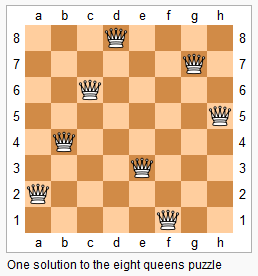
\includegraphics[width=0.3\textwidth]{n-queen.png}

    现在给定整数 $n$,请你输出所有的满足条件的棋子摆法。

    输入格式:

    共一行,包含整数 $n$。

    输出格式:

    每个解决方案占 $n$ 行,每行输出一个长度为 $n$ 的字符串,用来表示完整的棋盘状态。
    其中 \inlinecode{.} 表示某一个位置的方格状态为空,\inlinecode{Q} 表示某一个位置的方格上摆着皇后。每个方案输出完成后,输出一个空行。\textbf{注意:行末不能有多余空格。}输出方案的顺序任意,只要不重复且没有遗漏即可。

    数据范围:

    $1 \le n \le 9$

    \begin{inputblock}
        \inlinecode{4}
    \end{inputblock}
    \begin{outputblock}
        \inlinecode{.Q..} \\
        \inlinecode{...Q} \\
        \inlinecode{Q...} \\
        \inlinecode{..Q.} \\

        \inlinecode{..Q.} \\
        \inlinecode{Q...} \\
        \inlinecode{...Q} \\
        \inlinecode{.Q..}
    \end{outputblock}
\end{titledbox}

有两种解法,第一种:因发现每一行每一列有且仅有一个皇后,可以枚举每一行,来看看可以将皇后放置在第几列。

\begin{mycpptwocol}[n-皇后问题:解法一]
    #include <stdio.h>
    #include <stdlib.h>
    #include <string.h>
    #include <stdbool.h>

    #define N 20

    char g[N][N];
    bool col[N];
    bool dg[N];
    bool udg[N];

    void dfs(int u, int n) {
        if (u == n) {
            for (int i = 0; i < n; i++) {
                puts(g[i]);
            }
            printf("\n");
            return;
        }
        for (int i = 0; i < n; i++) {
            if (col[i] || dg[u + i] || udg[u - i + n]) {
                continue;
            }
            g[u][i] = 'Q';
            col[i] = dg[u + i] = udg[u - i + n] = true;
            dfs(u + 1, n);
            g[u][i] = '.';
            col[i] = dg[u + i] = udg[u - i + n] = false;
        }
    }

    int main() {
        int n;
        scanf("%d", &n);
        for (int i = 0; i < n; i++) {
            for (int j = 0; j < n; j++) {
                g[i][j] = '.';
            }
        }
        dfs(0,  n);
        return 0;
    }
\end{mycpptwocol}

解法二:从左上角开始枚举每一个格子,每个格子有两种状态(放或者不放),在枚举过程中检查每一个格子是否可以继续放置。若皇后数量已经达到最大数量则找到了一个方案

\begin{mycpptwocol}[n-皇后问题:解法二]
    #include <stdio.h>
    #include <stdlib.h>
    #include <string.h>
    #include <stdbool.h>

    #define N 20

    char g[N][N];
    bool row[N];
    bool col[N];
    bool dg[N];
    bool udg[N];

    void dfs(int x, int y, int s, int n) {
        if (y == n) {
            y = 0;
            x++;
        }
        if (x == n) {
            if (s == n) {
                for (int i = 0; i < n; i++) {
                    puts(g[i]);
                }
                puts("");
            }
            return;
        }
        // do not put queen here
        dfs(x, y + 1, s, n);

        // put queen here
        if (!row[x] && !col[y] && !dg[x + y] && !udg[x - y + n]) {
            g[x][y] = 'Q';
            row[x] = col[y] = dg[x + y] = udg[x - y + n] = true;
            dfs(x, y + 1, s + 1, n);
            g[x][y] = '.';
            row[x] = col[y] = dg[x + y] = udg[x - y + n] = false;
        }
    }

    int main() {
        int n;
        scanf("%d", &n);
        for (int i = 0; i < n; i++) {
            for (int j = 0; j < n; j++) {
                g[i][j] = '.';
            }
        }
        dfs(0, 0, 0, n);
        return 0;
    }
\end{mycpptwocol}


\section{BFS}

宽度优先搜索的基本思路是初始化一个队列,需要决定队列中存储的是什么。进入队列循环后从对头弹出元素 $t$ 之后,选择 $t$ 可拓展的节点之后将拓展节点入队。

\subsection{AcWing 844. 走迷宫}
\begin{titledbox}{AcWing 844. 走迷宫}
    给定一个 $n \times m$ 的二维整数数组,用来表示一个迷宫,数组中只包含 $0$ 或 $1$,其中 $0$ 表示可以走的路,$1$ 表示不可通过的墙壁。最初,有一个人位于左上角 $(1, 1)$ 处,已知该人每次可以向上、下、左、右任意一个方向移动一个位置。请问,该人从左上角移动至右下角 $(n, m)$ 处,至少需要移动多少次。数据保证 $(1, 1)$ 处和 $(n, m)$ 处的数字为 $0$,且一定至少存在一条通路。

    输入格式:

    第一行包含两个整数 $n$ 和 $m$。接下来 $n$ 行,每行包含 $m$ 个整数($0$ 或 $1$),表示完整的二维数组迷宫。

    输出格式:

    输出一个整数,表示从左上角移动至右下角的最少移动次数。

    数据范围:

    $1 \le n, m \le 100$

    \begin{inputblock}
        \inlinecode{5 5} \\
        \inlinecode{0 1 0 0 0} \\
        \inlinecode{0 1 0 1 0} \\
        \inlinecode{0 0 0 0 0} \\
        \inlinecode{0 1 1 1 0} \\
        \inlinecode{0 0 0 1 0}
    \end{inputblock}
    \begin{outputblock}
        \inlinecode{8}
    \end{outputblock}
\end{titledbox}

\begin{mycpptwocol}[BFS 走迷宫]
    #include <stdio.h>
    #include <stdlib.h>

    #define N 110

    int g[N][N];
    int d[N][N];

    typedef struct {
        int x;
        int y;
    } Pair;

    Pair queue[N * N];

    int bfs(int n, int m) {
        int head = 0;
        int tail = 0;
        Pair init = {0, 0};
        queue[tail++] = init;
        memset(d, -1, sizeof(d));
        d[0][0] = 0;

        int dx[4] = {0, 1, 0, -1};
        int dy[4] = {1, 0, -1, 0};

        while (head <= tail) {
            Pair t = queue[head++];
            for (int i = 0; i < 4; i++) {
                int x = t.x + dx[i];
                int y = t.y + dy[i];
                if (x >= 0 && x < n && y >= 0 && y < m && d[x][y] == -1 && g[x][y] == 0) {
                    queue[tail++] = (Pair){x, y};
                    d[x][y] = d[t.x][t.y] + 1;
                }
            }
        }
        return d[n - 1][m - 1];
    }

    int main() {
        int n;
        int m;
        scanf("%d %d", &n, &m);
        for (int i = 0; i < n; i++) {
            for (int j = 0; j < m; j++) {
                scanf("%d", &g[i][j]);
            }
        }
        printf("%d", bfs(n, m));
        return 0;
    }
\end{mycpptwocol}

\begin{information}
    若想要输出最短路径,则可以开一个数组 \inlinecode{Pair prev[N][N];} 来存储每一个点的前一个节点(在扩展 $t$ 时可以操作),最后从后往前循环输出即可。
\end{information}

\subsection{AcWing 845. 八数码}
\begin{titledbox}{AcWing 845. 八数码}
    在一个 $3 \times 3$ 的网格中,$1 \sim 8$ 这 $8$ 个数字和一个 \inlinecode{x} 恰好不重不漏地分布在这 $3 \times 3$ 的网格中。

    例如:

    \inlinecode{1 2 3} \\
    \inlinecode{x 4 6} \\
    \inlinecode{7 5 8}

    在游戏过程中,可以把 \inlinecode{x} 与其上、下、左、右四个方向之一的数字交换(如果存在)。
    我们的目的是通过交换,使得网格变为如下排列(称为正确排列):

    \inlinecode{1 2 3} \\
    \inlinecode{4 5 6} \\
    \inlinecode{7 8 x}

    例如,示例中图形就可以通过让 \inlinecode{x} 先后与右、下、右三个方向的数字交换成功得到正确排列。
    交换过程如下:

    \inlinecode{1 2 3} \hspace{1em} \inlinecode{1 2 3} \hspace{1em} \inlinecode{1 2 3} \hspace{1em} \inlinecode{1 2 3} \\
    \inlinecode{x 4 6} \hspace{1em} \inlinecode{4 x 6} \hspace{1em} \inlinecode{4 5 6} \hspace{1em} \inlinecode{4 5 6} \\
    \inlinecode{7 5 8} \hspace{1em} \inlinecode{7 5 8} \hspace{1em} \inlinecode{7 x 8} \hspace{1em} \inlinecode{7 8 x}

    现在,给你一个初始网格,请你求出得到正确排列至少需要进行多少次交换。

    输入格式:

    输入占一行,将 $3 \times 3$ 的初始网格描绘出来。例如,如果初始网格如下所示:

    \inlinecode{1 2 3} \\
    \inlinecode{x 4 6} \\
    \inlinecode{7 5 8}

    则输入为:\inlinecode{1 2 3 x 4 6 7 5 8}

    输出格式:

    输出占一行,包含一个整数,表示最少交换次数。如果不存在解决方案,则输出 $-1$。

    \begin{inputblock}
        \inlinecode{2 3 4 1 5 x 7 6 8}
    \end{inputblock}
    \begin{outputblock}
        \inlinecode{19}
    \end{outputblock}
\end{titledbox}


\section{树与图的存储}
树是一种特殊的图(无环联通图);图分为有向图和无向图,无向图又可看作是特殊的有向图(每两个相连的节点之间有两条分别指向对方的边)。所以树和图均可统一看作图,故此处仅讨论有向图的存储方式。

有向图的存储有两种方式:
\begin{description}
    \item[邻接矩阵]
    使用二维数组存储图 \inlinecode{g[a][b]} 表示边 $a \rightarrow b$ 上的权重,若无权图则表示边的存在性。空间复杂度为 \bigo{$n^2$} ,比较浪费空间,常用来存储稠密图。
    \item[邻接表]
    使用链表的形式,每一个节点对应一个单链表来存储由该点出发可以走到的所有点。
\end{description}
由上可见,邻接表的存储方式和Hash表的拉链法是一样的。


\section{树与图的深度优先遍历}

模版如下:
\begin{mycpptwocol}[dfs in tree and graphic]
    int h[N], e[M], ne[M], idx;
    bool st[N]; // 状态数组,存储节点时候已访问

    void add(int a, int b) {
        e[++idx] = b;
        ne[idx] = h[a];
        h[a] = idx;
    }

    void dfs(int u) {
        st[u] = true;
        for (int i = h[t]; i != -1; i = ne[i]) {
            int j = e[i];
            if (!st[j] && check(j)) {
                dfs(j);
            }
        }
    }
\end{mycpptwocol}
其中,14行的 \inlinecode{check(j)} 的作用是剪枝。

\subsection{AcWing 846. 树的重心}
\begin{titledbox}{AcWing 846. 树的重心}
    给定一棵树,树中包含 $n$ 个结点(编号 $1 \sim n$)和 $n-1$ 条无向边。请你找到树的重心,并输出将重心删除后,剩余各个连通块中点数的最大值。

    重心定义:重心是指树中的一个结点,如果将这个点删除后,剩余各个连通块中点数的最大值最小,那么这个节点被称为树的重心。

    输入格式:

    第一行包含整数 $n$,表示树的结点数。接下来 $n-1$ 行,每行包含两个整数 $a$ 和 $b$,表示点 $a$ 和点 $b$ 之间存在一条边。

    输出格式:

    输出一个整数 $m$,表示将重心删除后,剩余各个连通块中点数的最大值。

    数据范围:

    $1 \le n \le 10^5$

    \begin{inputblock}
        \inlinecode{9} \\
        \inlinecode{1 2} \\
        \inlinecode{1 7} \\
        \inlinecode{1 4} \\
        \inlinecode{2 8} \\
        \inlinecode{2 5} \\
        \inlinecode{4 3} \\
        \inlinecode{3 9} \\
        \inlinecode{4 6}
    \end{inputblock}
    \begin{outputblock}
        \inlinecode{4}
    \end{outputblock}
\end{titledbox}

\begin{mycpptwocol}[树的DFS]
    #include <stdio.h>
    #include <stdlib.h>
    #include <stdbool.h>

    #define N 100010

    int h[N], e[N], ne[N], idx;
    bool st[N];
    int ans = N;

    void add(int a, int b) {
        e[++idx] = b;
        ne[idx] = h[a];
        h[a] = idx;
    }

    int max(int a, int b) {
        return a > b ? a : b;
    }

    int min(int a, int b) {
        return a < b ? a : b;
    }

    // 返回以节点u为根的子树的节点数
    int dfs(int u, int n) {
        st[u] = true;

        int sum = 1; // 计入当前节点
        // res为去掉u之后所有连通块中节点数最大值
        int res = 0;
        for (int i = h[u]; i != -1; i = ne[i]) {
            int j = e[i];
            if (!st[j]) {
                int s = dfs(j, n);
                res = max(res, s);
                sum += s;
            }
        }
        res = max(res, n - sum);
        ans = min(ans, res);
        return sum;
    }

    int main() {
        memset(h, -1, sizeof(h));
        int n;
        scanf("%d", &n);

        int a;
        int b;
        for (int i = 0; i < n - 1; i++) {
            scanf("%d %d", &a, &b);
            add(a, b);
            add(b, a);
        }
        dfs(1, n);
        printf("%d", ans);
        return 0;
    }
\end{mycpptwocol}


\section{树与图的广度优先遍历}

\subsection{AcWing 847. 图中点的层次}
\begin{titledbox}{AcWing 847. 图中点的层次}
    给定一个 $n$ 个点 $m$ 条边的有向图,图中可能存在重边和自环。所有边的长度都是 $1$,点的编号为 $1 \sim n$。请你求出 $1$ 号点到 $n$ 号点的最短距离,如果从 $1$ 号点无法走到 $n$ 号点,输出 $-1$。

    输入格式:

    第一行包含两个整数 $n$ 和 $m$。接下来 $m$ 行,每行包含两个整数 $a$ 和 $b$,表示存在一条从 $a$ 走到 $b$ 的长度为 $1$ 的边。

    输出格式:

    输出一个整数,表示 $1$ 号点到 $n$ 号点的最短距离。

    数据范围:

    $1 \le n,m \le 10^5$

    \begin{inputblock}
        \inlinecode{4 5} \\
        \inlinecode{1 2} \\
        \inlinecode{2 3} \\
        \inlinecode{3 4} \\
        \inlinecode{1 3} \\
        \inlinecode{1 4}
    \end{inputblock}
    \begin{outputblock}
        \inlinecode{1}
    \end{outputblock}
\end{titledbox}

\begin{mycpptwocol}[图的BFS]
    #include <stdio.h>
    #include <stdlib.h>

    #define N 100010

    int h[N], e[N], ne[N], idx;

    int d[N];

    void add(int a, int b) {
        e[++idx] = b;
        ne[idx] = h[a];
        h[a] = idx;
    }

    int bfs(int n) {
        int *q = (int *)calloc(n, sizeof(int));
        int tt = 0;
        int hh = 0;
        q[tt++] = 1;
        d[1] = 0;
        while (hh < tt) {
            int t = q[hh++];
            for (int i = h[t]; i != -1; i = ne[i]) {
                int j = e[i];
                if (d[j] == -1) {
                    d[j] = d[t] + 1;
                    q[tt++] = j;
                }
            }
        }
        return d[n];
    }

    int main() {
        memset(h, -1, sizeof(h));
        memset(d, -1, sizeof(d));
        int n;
        int m;
        scanf("%d %d", &n, &m);
        int a;
        int b;
        while (m--) {
            scanf("%d %d", &a, &b);
            add(a, b);
        }
        printf("%d", bfs(n));
        return 0;
    }
\end{mycpptwocol}


\section{拓扑排序}

\subsection{AcWing 848. 有向图的拓扑序列}
\begin{titledbox}{AcWing 848. 有向图的拓扑序列}
    给定一个 $n$ 个点 $m$ 条边的有向图,点的编号是 $1$ 到 $n$,图中可能存在重边和自环。请输出任意一个该有向图的拓扑序列,如果拓扑序列不存在,则输出 $-1$。若一个由图中所有点构成的序列 $A$ 满足:对于图中的每条边 $(x, y)$,$x$ 在 $A$ 中都出现在 $y$ 之前,则称 $A$ 是该图的一个拓扑序列。

    输入格式:

    第一行包含两个整数 $n$ 和 $m$。接下来 $m$ 行,每行包含两个整数 $x$ 和 $y$,表示存在一条从点 $x$ 到点 $y$ 的有向边 $(x, y)$。

    输出格式:

    共一行,如果存在拓扑序列,则输出任意一个合法的拓扑序列即可。否则输出 $-1$。

    数据范围:

    $1 \le n,m \le 10^5$

    \begin{inputblock}
        \inlinecode{3 3} \\
        \inlinecode{1 2} \\
        \inlinecode{2 3} \\
        \inlinecode{1 3} \\
    \end{inputblock}
    \begin{outputblock}
        \inlinecode{1 2 3}
    \end{outputblock}
\end{titledbox}

\begin{mycpptwocol}[拓扑排序]
    #include <stdio.h>
    #include <stdlib.h>
    #include <stdbool.h>

    #define N 100010

    int h[N], e[N], ne[N], idx;
    int degree[N];

    int q[N], hh, tt;

    void Add(int a, int b) {
        e[++idx] = b;
        ne[idx] = h[a];
        h[a] = idx;
        degree[b]++;
    }

    bool TopoSort(int n) {
        for (int i = 1; i <= n; i++) {
            if (degree[i] == 0) {
                q[tt++] = i;
            }
        }
        while (hh < tt) {
            int t = q[hh++];
            for (int i = h[t]; i != -1; i = ne[i]) {
                int j = e[i];
                degree[j]--;
                if (degree[j] == 0) {
                    q[tt++] = j;
                }
            }
        }
        return tt == n;
    }

    int main() {
        memset(h, -1, sizeof(h));
        int n;
        int m;
        scanf("%d %d", &n, &m);
        int a;
        int b;
        while (m--) {
            scanf("%d %d", &a, &b);
            Add(a, b);
        }
        if (TopoSort(n)) {
            int hh = 0;
            while (hh < tt) {
                printf("%d ", q[hh++]);
            }
        } else {
            puts("-1");
        }
        return 0;
    }
\end{mycpptwocol}


\section{有向图的最短路问题}
这一节将关注在图的最短路的求解上,最短路问题及其常见方法如下,其中 $n$ 表示点数,$m$ 表示边数

\begin{enumerate}
    \item 单源最短路:求一个点到其他所有点的最短路
    \begin{itemize}
        \item 所有边权都是正数:1. 朴素 Dijkstra 算法\bigo{$n^2$},与边数无关,适合稠密图 2. 堆优化版的 Dijkstra 算法 \bigo{$m\log{}n$} 稀疏图:$m$ 与 $n$ 量级相同
        \item 存在负权边:1. Bellman-Ford 算法 \bigo{$nm$} 2. SPFA \bigo{$m$}最坏 \bigo{$nm$}
    \end{itemize}
    \item 多源汇最短路:起点和终点不确定,问 $a$ 到 $b$ 的最短路
    \begin{itemize}
        \item Floyd 算法 \bigo{$n^3$}
    \end{itemize}
\end{enumerate}

\subsection{AcWing 849. Dijkstra 求最短路 I}

朴素版的 Dijkstra 算法:
\begin{myenum}
    \item 用邻接矩阵存储图;\inlinecode{g[N][N]}
    \item 用一个数组存储每一个点到起始点的距离\inlinecode{d[N]};
    \item \inlinecode{st[N]},存储每一个点是否已经找到了最短路
\end{myenum}

算法逻辑:
\begin{myenum}
    \item 将距离数组初始化为\inlinecode{d[i] = $+\infty$; d[k] = 0;} $k$ 表示起始点
    \item 从第$0$个点到第$n - 1$个点,找到距离当前点最近的下一个点(遍历$1 - n$) \inlinecode{t; st[t] = true;}
    \item 用$t$更新其他点的距离(遍历$1 - n$)
\end{myenum}

\begin{titledbox}{AcWing 849. Dijkstra 求最短路 I}
    给定一个 $n$ 个点 $m$ 条边的有向图,图中可能存在重边和自环,所有边权均为正值。请你求出 $1$ 号点到 $n$ 号点的最短距离,如果无法从 $1$ 号点走到 $n$ 号点,则输出 $-1$。

    输入格式:

    第一行包含整数 $n$ 和 $m$。接下来 $m$ 行每行包含三个整数 $x,y,z$,表示存在一条从点 $x$ 到点 $y$ 的有向边,边长为 $z$。

    输出格式:

    输出一个整数,表示 $1$ 号点到 $n$ 号点的最短距离。如果路径不存在,则输出 $-1$。

    数据范围:

    $1 \le n \le 500$, $1 \le m \le 10^5$,图中涉及边长均不超过10000。

    \begin{inputblock}
        \inlinecode{3 3} \\
        \inlinecode{1 2 2} \\
        \inlinecode{2 3 1} \\
        \inlinecode{1 3 4}
    \end{inputblock}
    \begin{outputblock}
        \inlinecode{3}
    \end{outputblock}
\end{titledbox}

\begin{mycpptwocol}[朴素 Dijkstra 算法]
    #include <stdio.h>
    #include <stdlib.h>
    #include <stdbool.h>
    #include <string.h>

    #define N 510
    #define INF 0x3f3f3f3f

    int g[N][N];
    int d[N];
    bool st[N];

    int min(int a, int b) {
        return a < b ? a : b;
    }

    int dijkstra(int k, int n) {
        memset(d, 0x3f, sizeof(d));
        d[1] = 0;
        for (int i = 0; i < n - 1; i++) {
            int t = -1;
            for (int j = 1; j <= n; j++) {
                if (!st[j] && (t == -1 || d[t] > d[j])) {
                    t = j;
                }
            }

            st[t] = true;
            for (int j = 1; j <= n; j++) {
                d[j] = min(d[j], d[t] + g[t][j]);
            }
        }

        return d[n] == INF ? -1 : d[n];
    }

    int main() {
        memset(g, 0x3f, sizeof(g));
        int n;
        int m;
        scanf("%d %d", &n, &m);
        while (m--) {
            int a, b, c;
            scanf("%d %d %d", &a, &b, &c);
            if (a == b) {
                continue;
            }
            g[a][b] = min(g[a][b], c);
        }
        printf("%d", dijkstra(1, n));
        return 0;
    }
\end{mycpptwocol}

\subsection{AcWing 850. Dijkstra 求最短路 II}

注意到在朴素版的 Dijkstra 算法中需要找到当前节点之后的所有节点中距离最小的那个点的复杂度是 \bigo{$n$},而堆中寻找最小值的复杂度则为 \bigo{$1$}。所以可以用堆来优化这个过程。后面用到了修改堆中元素,为了简单起见,直接插入即可。

如果稠密图中 $n$ 的量为 $10^5$ 时 \bigo{$n^2$} 将会超时,所以选择使用堆对其进行优化,将其降低到 \bigo{$m \log{}n$}

\begin{titledbox}{AcWing 850. Dijkstra 求最短路 II}
    给定一个 $n$ 个点 $m$ 条边的有向图,图中可能存在重边和自环,所有边权均为正值。请你求出 $1$ 号点到 $n$ 号点的最短距离,如果无法从 $1$ 号点走到 $n$ 号点,则输出 $-1$。

    输入格式:

    第一行包含整数 $n$ 和 $m$。接下来 $m$ 行每行包含三个整数 $x,y,z$,表示存在一条从点 $x$ 到点 $y$ 的有向边,边长为 $z$。

    输出格式:

    输出一个整数,表示 $1$ 号点到 $n$ 号点的最短距离。如果路径不存在,则输出 $-1$。

    数据范围:

    $1 \le n, m \le 1.5 \times 10^5$,图中涉及边长均不小于 0,且不超过 10000。

    \begin{inputblock}
        \inlinecode{3 3} \\
        \inlinecode{1 2 2} \\
        \inlinecode{2 3 1} \\
        \inlinecode{1 3 4}
    \end{inputblock}
    \begin{outputblock}
        \inlinecode{3}
    \end{outputblock}
\end{titledbox}

\subsection{bellman-ford}
处理有负权边的图,如果有负权回路的话最短路不一定存在。所以一般不能有负权回路。

算法逻辑:
\begin{myenum}
    \item 循环 $n$ 个点
    \item 循环所有边 \inlinecode{a, b, w: dist[b] = min(dist[b], dist[a] + w)} 更新所有距离
\end{myenum}

\begin{algorithm}[H] %or another one check
    \caption{Bellman-Ford}
    \SetAlgoLined
    \KwData{graph $G$ and start point $s$}
    \KwResult{Shortest path from $s$ to the end}
    \For{each vertex $v \neq s$ in $V(G)$}{
        $d(v) \leftarrow \infty$
    }
    $d(s) \leftarrow 0$\\
\end{algorithm}

因为算法特点存储图时不必使用邻接矩阵或者邻接表,开一个结构体数组:

\begin{mycpponecol}[边集]
    struct {
        int a;
        int b;
        int w;
    } Edges[N]
\end{mycpponecol}

只要能够遍历到所有边即可。可以证明,该算法完成后一定有\textbf{三角不等式}:\inlinecode{dist[b] <= dist[a] + w}成立
更新距离数组的过程叫做\textbf{松弛操作}。

第一个循环中,如果当前迭代了 $k$ 次,此时的 \inlinecode{dist} 数组表示的是从 $1$ 号点经过不超过 $k$ 条边走到每个点的距离,所以可以用这个原理来找负环,迭代到第 $n$ 次仍能更新则表示有 $n+1$ 个点,但实际只有 $n$ 个点,所以一定存在负环。但一般不用该算法找负环。

\subsubsection{AcWing 853. 有边数限制的最短路}
\begin{titledbox}{AcWing 853. 有边数限制的最短路}
    给定一个 $n$ 个点 $m$ 条边的有向图,图中可能存在重边和自环, \textbf{边权可能为负数}。 请你求出从 $1$ 号点到 $n$ 号点的最多经过 $k$ 条边的最短距离,如果无法从 $1$ 号点走到 $n$ 号点,输出 \inlinecode{impossible}。 注意:图中可能 \textbf{存在负权回路}。

    输入格式:

    第一行包含三个整数 $n,m,k$。 接下来 $m$ 行,每行包含三个整数 $x,y,z$,表示存在一条从点 $x$ 到点 $y$ 的有向边,边长为 $z$。

    输出格式:

    输出一个整数,表示从 $1$ 号点到 $n$ 号点的最多经过 $k$ 条边的最短距离。 如果不存在满足条件的路径,则输出 \inlinecode{impossible}。

    数据范围:

    $1 \le n,k \le 500$, $1 \le m \le 10000$, 任意边长的绝对值不超过 $10000$。

    \begin{inputblock}
        \inlinecode{3 3 1} \\
        \inlinecode{1 2 1} \\
        \inlinecode{2 3 1} \\
        \inlinecode{1 3 3}
    \end{inputblock}
    \begin{outputblock}
        \inlinecode{3}
    \end{outputblock}
\end{titledbox}

\begin{mycpptwocol}[Bellman-ford]
    #include <stdio.h>
    #include <stdlib.h>
    #include <string.h>

    #define N 10010

    typedef struct {
        int a;
        int b;
        int c;
    } Edge;

    int d[N];
    int backup[N];

    int min(int a, int b) {
        return a < b ? a : b;
    }

    int Bellman_ford(Edge *edges, int k, int m, int n) {
        memset(d, 0x3f, sizeof(d));
        d[1] = 0;
        for (int i = 0; i < k; i++) {
            memcpy(backup, d, sizeof(d));
            for (int j = 0; j < m; j++) {
                d[edges[j].b] = min(d[edges[j].b], backup[edges[j].a] + edges[j].c);
            }
        }
        return d[n];
    }

    int main() {
        int n, m, k;
        scanf("%d %d %d", &n, &m, &k);
        Edge *edges = (Edge *)calloc(m, sizeof(Edge));
        for (int i = 0; i < m; i++) {
            scanf("%d %d %d", &edges[i].a, &edges[i].b, &edges[i].c);
        }
        int t = Bellman_ford(edges, k, m, n);
        if (t >= 0x3f3f3f3f / 2) {
            puts("impossible");
        } else {
            printf("%d", t);
        }
        free(edges);
        return 0;
    }
\end{mycpptwocol}

\subsection{SPFA}
SPFA 算法是对 Bellman-Ford 算法的优化,在松弛操作中,不一定每一次都会对该点的距离减小有所贡献,只有与之相连的前驱节点距离减小了,此时才有可能有所贡献。

用一个 BFS 来做优化,队列中存储所有变小了距离的节点,其中的状态数组标识某个节点是否在队列中,出队时要清空标识位。

\begin{algorithm}[H] %or another one check
    \caption{SPFA(Shortest Path Faster Algorithm)}
    \SetAlgoLined
    \KwData{graph $G$ and start point $s$}
    \KwResult{Shortest path from $s$ to the end}
    init a FIFO queue $Q$\;
    \For{each vertex $v \neq s$ in $V(G)$}{
        $d(v) \leftarrow \infty$
    }
    $d(s) \leftarrow 0$\\
    push $s$ into $Q$\\
    \While{$Q$ is not empty}{
        $u \leftarrow \text{poll } Q$\\
        \For{each edge ($u, v$) in $E(G)$} {
            \If{$d(u) + w(u, v) < d(v)$}{
                $d(v) \leftarrow d(u) + w(u, v)$\\
                \If{$v$ is not in $Q$}{
                    push $v$ into $Q$
                }
            }
        }
    }
\end{algorithm}

\subsubsection{AcWing 851. SPFA 求最短路}

\begin{titledbox}{AcWing 851. SPFA 求最短路}
    给定一个 $n$ 个点 $m$ 条边的有向图,图中可能存在重边和自环, \textbf{边权可能为负数}。 请你求出 $1$ 号点到 $n$ 号点的最短距离,如果无法从 $1$ 号点走到 $n$ 号点,则输出 \inlinecode{impossible}。
    数据保证不存在负权回路。

    输入格式:

    第一行包含整数 $n$ 和 $m$。 接下来 $m$ 行每行包含三个整数 $x,y,z$,表示存在一条从点 $x$ 到点 $y$ 的有向边,边长为 $z$。

    输出格式:

    输出一个整数,表示 $1$ 号点到 $n$ 号点的最短距离。如果路径不存在,则输出 \inlinecode{impossible}。

    数据范围:

    $1 \le n,m \le 10^5$, 图中涉及边长绝对值均不超过 $10000$。

    \begin{inputblock}
        \inlinecode{3 3} \\
        \inlinecode{1 2 5} \\
        \inlinecode{2 3 -3} \\
        \inlinecode{1 3 4}
    \end{inputblock}
    \begin{outputblock}
        \inlinecode{2}
    \end{outputblock}
\end{titledbox}

\begin{mycpptwocol}[SPFA]
    #include <stdio.h>
    #include <stdlib.h>
    #include <stdbool.h>
    #include <string.h>

    #define N 100010

    int h[N];
    int e[N];
    int ne[N];
    int w[N];
    int idx;

    int d[N];
    bool st[N];

    int q[N];
    int hh;
    int tt;

    int add(int a, int b, int c) {
        e[++idx] = b;
        ne[idx] = h[a];
        h[a] = idx;
        w[idx] = c;
    }

    int spfa(int n, int m) {
        memset(d, 0x3f, sizeof(d));
        d[1] = 0;
        q[tt++] = 1;
        st[1] = true;

        while (hh < tt) {
            int t = q[hh++];
            st[t] = false;
            for (int i = h[t]; i != -1; i = ne[i]) {
                int j = e[i];
                if (d[j] > d[t] + w[i]) {
                    d[j] = d[t] + w[i];
                    if (!st[j]) {
                        q[tt++] = j;
                        st[j] = true;
                    }
                }
            }
        }
        return d[n];
    }

    int main() {
        memset(h, -1, sizeof(h));
        int n, m;
        scanf("%d %d", &n, &m);
        while (m--) {
            int a, b, c;
            scanf("%d %d %d", &a, &b, &c);
            add(a, b, c);
        }
        int t = spfa(n, m);
        if (t == 0x3f3f3f3f) {
            printf("impossible");
        } else {
            printf("%d", t);
        }
        return 0;
    }
\end{mycpptwocol}

\subsubsection{AcWing 852. spfa 判断负环}

\begin{titledbox}{AcWing 852. spfa 判断负环}
    给定一个 $n$ 个点 $m$ 条边的有向图,图中可能存在重边和自环, \textbf{边权可能为负数}。 请你判断图中是否存在负权回路。

    输入格式:

    第一行包含整数 $n$ 和 $m$。 接下来 $m$ 行每行包含三个整数 $x,y,z$,表示存在一条从点 $x$ 到点 $y$ 的有向边,边长为 $z$。

    输出格式:

    如果图中 \textbf{存在} 负权回路,则输出 \inlinecode{Yes},否则输出 \inlinecode{No}。

    数据范围:

    $1 \le n \le 2000$, $1 \le m \le 10000$, 图中涉及边长绝对值均不超过 $10000$。

    \begin{inputblock}
        \inlinecode{3 3} \\
        \inlinecode{1 2 -1} \\
        \inlinecode{2 3 4} \\
        \inlinecode{3 1 -4}
    \end{inputblock}
    \begin{outputblock}
        \inlinecode{Yes}
    \end{outputblock}
\end{titledbox}

\subsection{Floyd}
求多源汇最短路,用邻接矩阵来存储 \inlinecode{d[i, j]}

\begin{mycpponecol}[Floyd 算法]
    for (int k = 1; k <= n; ++k) {
        for (int i = 1; i <= n; ++i) {
            for (int j = 1; j <= n; ++j) {
                d[i, j] = min(d[i, j], d[i, k] + d[k, j]);
            }
        }
    }
\end{mycpponecol}

初始时, \inlinecode{d[i, j]} 就是邻接矩阵,结束之后 \inlinecode{d[i, j]} 是最短路长度

\subsection{AcWing 854. Floyd 求最短路}

\begin{titledbox}{AcWing 854. Floyd 求最短路}
    给定一个 $n$ 个点 $m$ 条边的有向图,图中可能存在重边和自环,边权可能为负数。 再给定 $k$ 个询问,每个询问包含两个整数 $x$ 和 $y$,表示查询从点 $x$ 到点 $y$ 的最短距离,如果路径不存在,则输出 \inlinecode{impossible}。 数据保证图中不存在负权回路。

    输入格式:

    第一行包含三个整数 $n,m,k$。 接下来 $m$ 行,每行包含三个整数 $x,y,z$,表示存在一条从点 $x$ 到点 $y$ 的有向边,边长为 $z$。 接下来 $k$ 行,每行包含两个整数 $x,y$,表示询问点 $x$ 到点 $y$ 的最短距离。

    输出格式:

    共 $k$ 行,每行输出一个整数,表示询问的结果,若询问两点间不存在路径,则输出 \inlinecode{impossible}。

    数据范围:

    $1 \le n \le 200$, $1 \le k \le n^2$, $1 \le m \le 20000$, 图中涉及边长绝对值均不超过 $10000$。

    \begin{inputblock}
        \inlinecode{3 3 2} \\
        \inlinecode{1 2 1} \\
        \inlinecode{2 3 2} \\
        \inlinecode{1 3 1} \\
        \inlinecode{2 1} \\
        \inlinecode{1 3}
    \end{inputblock}
    \begin{outputblock}
        \inlinecode{impossible} \\
        \inlinecode{1}
    \end{outputblock}
\end{titledbox}

\begin{mycpptwocol}[Floyd]
    #include <stdio.h>
    #include <stdbool.h>
    #include <stdlib.h>
    #include <string.h>

    #define N 210
    #define INF 0x3f3f3f3f

    int g[N][N];

    int Min(int a, int b) {
        return a < b ? a : b;
    }

    void Floyd(int n) {
        for (int k = 1; k <= n; k++) {
            for (int i = 1; i <= n; i++) {
                for (int j = 1; j <= n; j++) {
                    g[i][j] = Min(g[i][j], g[i][k] + g[k][j]);
                }
            }
        }
    }

    int main() {
        int n, m, k;
        scanf("%d %d %d", &n, &m, &k);
        for (int i = 1; i <= n; i++) {
            for (int j = 1; j <= n; j++) {
                if (i == j) {
                    g[i][j] = 0;
                } else {
                    g[i][j] = INF;
                }
            }
        }
        while (m--) {
            int a, b, w;
            scanf("%d %d %d", &a, &b, &w);
            g[a][b] = Min(g[a][b], w);
        }
        Floyd(n);
        while (k--) {
            int a, b;
            scanf("%d %d", &a, &b);
            if (g[a][b] > INF / 2) {
                puts("impossible");
            } else {
                printf("%d\n", g[a][b]);
            }
        }
        return 0;
    }
\end{mycpptwocol}


\section{无向图的最小生成树问题}

\begin{myenum}
    \item 普里姆算法(Prim 算法)1. 朴素版 Prim(稠密图)\bigo{$n^2$} 2.堆优化版 Prim(稀疏图)\bigo{$m\log{} n$},一般用不到
    \item 克鲁斯卡尔算法(Kruskal 算法)\bigo{$m\log{} m$} 稀疏图
\end{myenum}

\subsection{AcWing 858. Prim 算法求最小生成树}
Prim 算法,与 Dijkstra 算法类似:

Prim 算法:

\begin{myenum}
    \item 用邻接矩阵存储图:\inlinecode{g[N][N]}
    \item 用一个数组存储每一个点到集合的距离 \inlinecode{d[N]}, 即存储该点所连接边的最小权重;
    \item 集合 \inlinecode{st[N]},存储当前已经在连通块中的点
\end{myenum}

算法逻辑:

\begin{myenum}
    \item 将距离数组初始化为 \inlinecode{d[i] = $+\infty$; d[0] = 1;}
    \item 从第 $0$ 个点到第 $n - 1$ 个点,找到集合外距离最近的点 \inlinecode{t; st[t] = true;}
    \item 用 $t$ 更新其他点到集合的距离
\end{myenum}

\begin{titledbox}{AcWing 858. Prim 算法求最小生成树}
    给定一个 $n$ 个点 $m$ 条边的无向图,图中可能存在重边和自环,边权可能为负数。 求最小生成树的树边权重之和,如果最小生成树不存在则输出 \inlinecode{impossible}。 给定一张边带权的无向图 $G=(V, E)$,其中 $V$ 表示图中点的集合,$E$ 表示图中边的集合,$n=|V|$,$m=|E|$。 由 $V$ 中的全部 $n$ 个顶点和 $E$ 中 $n-1$ 条边构成的无向连通子图被称为 $G$ 的一棵生成树,其中边的权值之和最小的生成树被称为无向图 $G$ 的最小生成树。

    输入格式:

    第一行包含两个整数 $n$ 和 $m$。 接下来 $m$ 行,每行包含三个整数 $u,v,w$,表示点 $u$ 和点 $v$ 之间存在一条权值为 $w$ 的边。

    输出格式:

    共一行,若存在最小生成树,则输出一个整数,表示最小生成树的树边权重之和,如果最小生成树不存在则输出 \inlinecode{impossible}。

    数据范围:

    $1 \le n \le 500$, $1 \le m \le 10^5$, 图中涉及边的边权的绝对值均不超过 $1000$。

    \begin{inputblock}
        \inlinecode{4 5} \\
        \inlinecode{1 2 1} \\
        \inlinecode{1 3 2} \\
        \inlinecode{1 4 3} \\
        \inlinecode{2 3 2} \\
        \inlinecode{3 4 4}
    \end{inputblock}
    \begin{outputblock}
        \inlinecode{6}
    \end{outputblock}
\end{titledbox}

\subsection{AcWing 859. Kruskal 算法求最小生成树}

\begin{myenum}
    \item 将所有边按照权重从小到大排序;\bigo{$m\log{} m$}
    \item 枚举每条边 $a$, $b$, 权重 $c$,如果 $a$ 和 $b$ 不连通,就把这条边加入到集合中。并查集
\end{myenum}

\begin{titledbox}{AcWing 859. Kruskal算法求最小生成树}
    给定一个 $n$ 个点 $m$ 条边的无向图,图中可能存在重边和自环,边权可能为负数。 求最小生成树的树边权重之和,如果最小生成树不存在则输出 \inlinecode{impossible}。 给定一张边带权的无向图 $G=(V, E)$,其中 $V$ 表示图中点的集合,$E$ 表示图中边的集合,$n=|V|$,$m=|E|$。 由 $V$ 中的全部 $n$ 个顶点和 $E$ 中 $n-1$ 条边构成的无向连通子图被称为 $G$ 的一棵生成树,其中边的权值之和最小的生成树被称为无向图 $G$ 的最小生成树。

    输入格式:

    第一行包含两个整数 $n$ 和 $m$。 接下来 $m$ 行,每行包含三个整数 $u,v,w$,表示点 $u$ 和点 $v$ 之间存在一条权值为 $w$ 的边。

    输出格式:

    共一行,若存在最小生成树,则输出一个整数,表示最小生成树的树边权重之和,如果最小生成树不存在则输出 \inlinecode{impossible}。

    数据范围:

    $1 \le n \le 10^5$, $1 \le m \le 2 \times 10^5$, 图中涉及边的边权的绝对值均不超过 $1000$。

    \begin{inputblock}
        \inlinecode{4 5} \\
        \inlinecode{1 2 1} \\
        \inlinecode{1 3 2} \\
        \inlinecode{1 4 3} \\
        \inlinecode{2 3 2} \\
        \inlinecode{3 4 4}
    \end{inputblock}
    \begin{outputblock}
        \inlinecode{6}
    \end{outputblock}
\end{titledbox}


\section{二分图}

定义:一个图的所有节点可以划分到两个集合中使得图中的边都只存在于集合之间的图称其为可二分的图。

性质:一个图是二分图,当且仅当一个图可以被二染色,当且仅当图中没有奇数环(环中边个数为奇数)

\begin{myenum}
    \item 染色法 \bigo{$n + m$}
    \item 匈牙利算法 最坏 \bigo{$mn$}, 实际运行时间一般远小于 \bigo{$mn$}
\end{myenum}


\subsection{AcWing 860. 染色法判定二分图}
\begin{titledbox}{AcWing 860. 染色法判定二分图}
    给定一个 $n$ 个点 $m$ 条边的无向图,图中可能存在重边和自环。 请你判断这个图是否是二分图。

    输入格式:

    第一行包含两个整数 $n$ 和 $m$。 接下来 $m$ 行,每行包含两个整数 $u$ 和 $v$,表示点 $u$ 和点 $v$ 之间存在一条边。

    输出格式:

    如果给定图是二分图,则输出 \inlinecode{Yes},否则输出 \inlinecode{No}。

    数据范围:

    $1 \le n,m \le 10^5$

    \begin{inputblock}
        \inlinecode{4 4} \\
        \inlinecode{1 3} \\
        \inlinecode{1 4} \\
        \inlinecode{2 3} \\
        \inlinecode{2 4}
    \end{inputblock}
    \begin{outputblock}
        \inlinecode{Yes}
    \end{outputblock}
\end{titledbox}

\subsection{匈牙利算法}

\subsection{AcWing 861. 二分图的最大匹配}

\begin{titledbox}{AcWing 861. 二分图的最大匹配}
    给定一个二分图,其中左半部包含 $n_1$ 个点(编号 $1 \sim n_1$),右半部包含 $n_2$ 个点(编号 $1 \sim n_2$),二分图共包含 $m$ 条边。 数据保证任意一条边的两个端点都不可能在同一部分中。 请你求出二分图的最大匹配数。

    \begin{description}
        \item [二分图的匹配:] \\
        给定一个二分图 $G$,在 $G$ 的一个子图 $M$ 中,$M$ 的边集 $\{E\}$ 中的任意两条边都不依附于同一个顶点,则称 $M$ 是一个匹配。
        \item [二分图的最大匹配:] \\
        所有匹配中包含边数最多的一组匹配被称为二分图的最大匹配,其边数即为最大匹配数。
    \end{description}

    输入格式:

    第一行包含三个整数 $n_1$、 $n_2$ 和 $m$。 接下来 $m$ 行,每行包含两个整数 $u$ 和 $v$,表示左半部点集中的点 $u$ 和右半部点集中的点 $v$ 之间存在一条边。

    输出格式:

    输出一个整数,表示二分图的最大匹配数。

    数据范围:

    $1 \le n_1,n_2 \le 500$, $1 \le u \le n_1$, $1 \le v \le n_2$, $1 \le m \le 10^5$

    \begin{inputblock}
        \inlinecode{2 2 4} \\
        \inlinecode{1 1} \\
        \inlinecode{1 2} \\
        \inlinecode{2 1} \\
        \inlinecode{2 2}
    \end{inputblock}
    \begin{outputblock}
        \inlinecode{2}
    \end{outputblock}
\end{titledbox}

    \chapter{数学知识}
本章主要分为四个部分:
\begin{myenum}
    \item 数论
    \item 组合计数
    \item 高斯消元
    \item 简单博弈论
\end{myenum}


\section{质数}
质数(Prime number),又称素数,指在大于1的自然数中,除了1和该数自身外,无法被其他自然数整除的数(也可定义为只有1与该数本身两个正因数的数)。大于1的自然数若不是素数,则称之为合数(也称为合成数)。算术基本定理确立了素数于数论里的核心地位:任何大于1的整数均可被表示成一串唯一素数之乘积。

\textbf{注意:}质数是从2开始定义的。所有$\leq 1$的整数既不是质数也不是合数。

\subsection{AcWing 866. 试除法判定质数}
\begin{titledbox}{AcWing 866. 试除法判定质数}
    给定 $n$ 个正整数 $a_i$,判定每个数是否是质数。

    输入格式:

    第一行包含整数 $n$。 接下来 $n$ 行,每行包含一个正整数 $a_i$。

    输出格式:

    共 $n$ 行,其中第 $i$ 行输出第 $i$ 个正整数 $a_i$ 是否为质数,是则输出 \inlinecode{Yes},否则输出 \inlinecode{No}。

    数据范围:

    $1 \le n \le 100$, $1 \le a_i \le 2^{31}-1$

    \begin{inputblock}
        \inlinecode{2} \\
        \inlinecode{2} \\
        \inlinecode{6}
    \end{inputblock}
    \begin{outputblock}
        \inlinecode{Yes} \\
        \inlinecode{No}
    \end{outputblock}
\end{titledbox}

从定义出发,可以使用简单的试除法来判定一个数是否为质数。

\begin{mycpptwocol}[朴素试除法]
    #include <stdio.h>
    #include <stdbool.h>

    bool IsPrime(int x) {
        if (x < 2) {
            return false;
        }
        for (int i = 2; i < x; i++) {
            if (x \% i == 0) {
                return false;
            }
        }
        return true;
    }

    int main() {
        int n;
        scanf("%d", &n);

        while (n--) {
            int x;
            scanf("%d", &x);
            printf("%s\n", IsPrime(x) ? "Yes" : "No");
        }

        return 0;
    }
\end{mycpptwocol}

显而易见的,该朴素试除法的时间复杂度为 \bigo{$n$},效率比较低。考虑到数的性质:
\begin{equation*}
    d \mid n \Rightarrow \frac{n}{d} \mid n
\end{equation*}
可见数的约数是成对出现的。所以枚举的过程中可以仅枚举一对中较小的那一个($d \le n / d \Leftrightarrow d \le \sqrt{n}$)即可。这样时间复杂度从\bigo{$n$}降低到\bigo{$\sqrt{n}$}。

\begin{mycpponecol}[优化试除法]
    for (int i = 2; i <= x / i; i++) {
        if (x \% i == 0) {
            return false;
        }
    }
\end{mycpponecol}

此外,判断条件那里还有两种不推荐的写法:
\begin{mylist}
    \item \inlinecode{i * i <= n} 这种会导致乘法的溢出
    \item \inlinecode{i <= sqrt(n)} 由于函数 \inlinecode{sqrt(n)} 计算速度很慢而不推荐
\end{mylist}

\subsection{AcWing 867. 分解质因数}
\begin{titledbox}{AcWing 867. 分解质因数}
    给定 $n$ 个正整数 $a_i$,将每个数分解质因数,并按照质因数从小到大的顺序输出每个质因数的底数和指数。

    输入格式:

    第一行包含整数 $n$。 接下来 $n$ 行,每行包含一个正整数 $a_i$。

    输出格式:

    对于每个正整数 $a_i$,按照从小到大的顺序输出其分解质因数后,每个质因数的底数和指数,每个底数和指数占一行。 每个正整数的质因数全部输出完毕后,输出一个空行。

    数据范围:

    $1 \le n \le 100$, $1 \le a_i \le 2 \times 10^9$

    \begin{inputblock}
        \inlinecode{2} \\
        \inlinecode{6} \\
        \inlinecode{8}
    \end{inputblock}
    \begin{outputblock}
        \inlinecode{2 1} \\
        \inlinecode{3 1} \\
        \\
        \inlinecode{2 3} \\

    \end{outputblock}
\end{titledbox}

\begin{mycpptwocol}
    #include <stdio.h>
    #include <stdlib.h>

    void split(int x)
        {
        for (int i = 2; i <= x; i++) {
            if (x \% i == 0) {
                int cnt = 0;
                while (x \% i == 0) {
                    x /= i;
                    cnt++;
                }
                printf("%d %d\n", i, cnt);
            }
        }
        printf("\n");
    }

    int main()
        {
        int n;
        scanf("%d", &n);
        while (n--) {
            int x;
            scanf("%d", &x);
            split(x);
        }
        return 0;
    }
\end{mycpptwocol}

\subsection{AcWing 868. 筛质数}
\begin{titledbox}{AcWing 868. 筛质数}
    给定一个正整数 $n$,请你求出 $1 \sim n$ 中质数的个数。

    输入格式:

    共一行,包含整数 $n$。

    输出格式:

    共一行,包含一个整数,表示 $1 \sim n$ 中质数的个数。

    数据范围:

    $1 \le n \le 10^6$

    \begin{inputblock}
        \inlinecode{8}
    \end{inputblock}
    \begin{outputblock}
        \inlinecode{4}
    \end{outputblock}
\end{titledbox}


\section{约数}

\subsection{AcWing 869. 试除法求约数}
\begin{titledbox}{AcWing 869. 试除法求约数}
    给定 $n$ 个正整数 $a_i$,对于每个整数 $a_i$,请你按照从小到大的顺序输出它的所有约数。

    输入格式:

    第一行包含整数 $n$。 接下来 $n$ 行,每行包含一个整数 $a_i$。

    输出格式:

    输出共 $n$ 行,其中第 $i$ 行输出第 $i$ 个整数 $a_i$ 的所有约数。

    数据范围:

    $1 \le n \le 100$, $2 \le a_i \le 2 \times 10^9$

    \begin{inputblock}
        \inlinecode{2} \\
        \inlinecode{6} \\
        \inlinecode{8}
    \end{inputblock}
    \begin{outputblock}
        \inlinecode{1 2 3 6} \\
        \inlinecode{1 2 4 8}
    \end{outputblock}
\end{titledbox}

\subsection{AcWing 870. 约数个数}

\begin{titledbox}{AcWing 870. 约数个数}
    给定 $n$ 个正整数 $a_i$,请你输出这些数的乘积的约数个数,答案对 $10^9+7$ 取模。

    输入格式:

    第一行包含整数 $n$。 接下来 $n$ 行,每行包含一个整数 $a_i$。

    输出格式:

    输出一个整数,表示所给正整数的乘积的约数个数,答案需对 $10^9+7$ 取模。

    数据范围:

    $1 \le n \le 100$, $1 \le a_i \le 2 \times 10^9$

    \begin{inputblock}
        \inlinecode{3} \\
        \inlinecode{2} \\
        \inlinecode{6} \\
        \inlinecode{8}
    \end{inputblock}
    \begin{outputblock}
        \inlinecode{12}
    \end{outputblock}
\end{titledbox}

\subsection{AcWing 871. 约数之和}
\begin{titledbox}{AcWing 871. 约数之和}
    给定 $n$ 个正整数 $a_i$,请你输出这些数的乘积的约数之和,答案对 $10^9+7$ 取模。

    输入格式:

    第一行包含整数 $n$。 接下来 $n$ 行,每行包含一个整数 $a_i$。

    输出格式:

    输出一个整数,表示所给正整数的乘积的约数之和,答案需对 $10^9+7$ 取模。

    数据范围:

    $1 \le n \le 100$, $1 \le a_i \le 2 \times 10^9$

    \begin{inputblock}
        \inlinecode{3} \\
        \inlinecode{2} \\
        \inlinecode{6} \\
        \inlinecode{8}
    \end{inputblock}
    \begin{outputblock}
        \inlinecode{252}
    \end{outputblock}
\end{titledbox}

\subsection{AcWing 872. 最大公约数}
\begin{titledbox}{AcWing 872. 最大公约数}
    给定 $n$ 对正整数 $a_i, b_i$,请你求出每对数的最大公约数。

    输入格式:

    第一行包含整数 $n$。 接下来 $n$ 行,每行包含一个整数对 $a_i,b_i$。

    输出格式:

    输出共 $n$ 行,每行输出一个整数对的最大公约数。

    数据范围:

    $1 \le n \le 10^5$, $1 \le a_i, b_i \le 2 \times 10^9$

    \begin{inputblock}
        \inlinecode{2} \\
        \inlinecode{3 6} \\
        \inlinecode{4 6}
    \end{inputblock}
    \begin{outputblock}
        \inlinecode{3} \\
        \inlinecode{2}
    \end{outputblock}
\end{titledbox}


\section{欧拉函数}

\subsection{AcWing 873. 欧拉函数}
\begin{titledbox}{AcWing 873. 欧拉函数}
    给定 $n$ 个正整数 $a_i$,请你求出每个数的欧拉函数。

    欧拉函数的定义:

    \begin{quote}
        $1 \sim N$ 中与 $N$ 互质的数的个数被称为欧拉函数,记为 $\varphi(N)$。

        若在算数基本定理中,$N = p_1^{a_1}p_2^{a_2}\dots p_m^{a_m}$,则:

        $\varphi (N)$ = $N \times \frac{p_1-1}{p_1} \times \frac{p_2-1}{p_2} \times \dots \times \frac{p_m-1}{p_m}$
    \end{quote}

    输入格式:

    第一行包含整数 $n$。 接下来 $n$ 行,每行包含一个正整数 $a_i$。

    输出格式:

    输出共 $n$ 行,每行输出一个正整数 $a_i$ 的欧拉函数。

    数据范围:

    $1 \le n \le 100$, $1 \le a_i \le 2 \times 10^9$

    \begin{inputblock}
        \inlinecode{3} \\
        \inlinecode{3} \\
        \inlinecode{6} \\
        \inlinecode{8}
    \end{inputblock}
    \begin{outputblock}
        \inlinecode{2} \\
        \inlinecode{2} \\
        \inlinecode{4}
    \end{outputblock}
\end{titledbox}

\subsection{AcWing 874. 筛法求欧拉函数}
\begin{titledbox}{AcWing 874. 筛法求欧拉函数}
    给定一个正整数 $n$,求 $1 \sim n$ 中每个数的欧拉函数之和。

    输入格式:

    共一行,包含一个整数 $n$。

    输出格式:

    共一行,包含一个整数,表示 $1 \sim n$ 中每个数的欧拉函数之和。

    数据范围:

    $1 \le n \le 10^6$

    \begin{inputblock}
        \inlinecode{6}
    \end{inputblock}
    \begin{outputblock}
        \inlinecode{12}
    \end{outputblock}
\end{titledbox}


\section{快速幂}

\subsection{AcWing 875. 快速幂}
\begin{titledbox}{AcWing 875. 快速幂}
    给定 $n$ 组 $a_i, b_i, p_i$,对于每组数据,求出 $a_i ^ {b_i} \bmod p_i$ 的值。

    输入格式:

    第一行包含整数 $n$。 接下来 $n$ 行,每行包含三个整数 $a_i, b_i, p_i$。

    输出格式:

    对于每组数据,输出一个结果,表示 $a_i ^ {b_i} \bmod p_i$ 的值。 每个结果占一行。

    数据范围:

    $1 \le n \le 100000$, $1 \le a_i,b_i,p_i \le 2 \times 10^9$

    \begin{inputblock}
        \inlinecode{2} \\
        \inlinecode{3 2 5} \\
        \inlinecode{4 3 9}
    \end{inputblock}
    \begin{outputblock}
        \inlinecode{4} \\
        \inlinecode{1}
    \end{outputblock}
\end{titledbox}

\subsection{AcWing 876. 快速幂求逆元}
\begin{titledbox}{AcWing 876. 快速幂求逆元}
    给定 $n$ 组 $a_i, p_i$,其中 $p_i$ 是质数,求 $a_i$ 模 $p_i$ 的乘法逆元,若逆元不存在则输出 \inlinecode{impossible}。\textbf{注意}:请返回在 $0 \sim p-1$ 之间的逆元。

    \begin{description}
        \item[乘法逆元的定义] \\
        若整数 $b,m$ 互质,并且对于任意的整数 $a$,如果满足 $b|a$,则存在一个整数 $x$,使得 $a/b≡a \times x \pmod m$,则称 $x$ 为 $b$ 的模 $m$ 乘法逆元,记为 $b^{-1} \pmod m$。\\
        $b$ 存在乘法逆元的充要条件是 $b$ 与模数 $m$ 互质。当模数 $m$ 为质数时,$b^{m-2}$ 即为 $b$ 的乘法逆元。
    \end{description}

    输入格式:

    第一行包含整数 $n$。 接下来 $n$ 行,每行包含一个数组 $a_i, p_i$,数据保证 $p_i$ 是质数。

    输出格式:

    输出共 $n$ 行,每组数据输出一个结果,每个结果占一行。 若 $a_i$ 模 $p_i$ 的乘法逆元存在,则输出一个整数,表示逆元,否则输出 \inlinecode{impossible}。

    数据范围:

    $1 \le n \le 10^5$, $1 \le a_i,p_i \le 2*10^9$

    \begin{inputblock}
        \inlinecode{4 3} \\
        \inlinecode{8 5} \\
        \inlinecode{6 3}
    \end{inputblock}
    \begin{outputblock}
        \inlinecode{1} \\
        \inlinecode{2} \\
        \inlinecode{impossible}
    \end{outputblock}
\end{titledbox}


\section{扩展欧几里得算法}

\subsection{AcWing 877. 扩展欧几里得算法}
\begin{titledbox}{AcWing 877. 扩展欧几里得算法}
    给定 $n$ 对正整数 $a_i, b_i$,对于每对数,求出一组 $x_i, y_i$,使其满足 $a_i \times x_i + b_i \times y_i = gcd(a_i, b_i)$。

    输入格式:

    第一行包含整数 $n$。 接下来 $n$ 行,每行包含两个整数 $a_i, b_i$。

    输出格式:

    输出共 $n$ 行,对于每组 $a_i, b_i$,求出一组满足条件的 $x_i, y_i$,每组结果占一行。 本题答案不唯一,输出任意满足条件的 $x_i, y_i$ 均可。

    数据范围:

    $1 \le n \le 10^5$, $1 \le a_i,b_i \le 2 \times 10^9$

    \begin{inputblock}
        \inlinecode{2} \\
        \inlinecode{4 6} \\
        \inlinecode{8 18}
    \end{inputblock}
    \begin{outputblock}
        \inlinecode{-1 1} \\
        \inlinecode{-2 1}
    \end{outputblock}
\end{titledbox}

\subsection{AcWing 878. 线性同余方程}
\begin{titledbox}{AcWing 878. 线性同余方程}
    给定 $n$ 组数据 $a_i,b_i,m_i$,对于每组数求出一个 $x_i$,使其满足 $a_i \times x_i \equiv b_i \pmod {m_i}$,如果无解则输出 \inlinecode{impossible}。

    输入格式:

    第一行包含整数 $n$。 接下来 $n$ 行,每行包含一组数据 $a_i,b_i,m_i$。

    输出格式:

    输出共 $n$ 行,每组数据输出一个整数表示一个满足条件的 $x_i$,如果无解则输出 \inlinecode{impossible}。 每组数据结果占一行,结果可能不唯一,输出任意一个满足条件的结果均可。 输出答案必须在 $int$ 范围之内。

    数据范围:

    $1 \le n \le 10^5$, $1 \le a_i,b_i,m_i \le 2 \times 10^9$

    \begin{inputblock}
        \inlinecode{2} \\
        \inlinecode{2 3 6} \\
        \inlinecode{4 3 5}
    \end{inputblock}
    \begin{outputblock}
        \inlinecode{impossible} \\
        \inlinecode{-3}
    \end{outputblock}
\end{titledbox}


\section{中国剩余定理}

\subsection{AcWing 204. 表达整数的奇怪方式}
\begin{titledbox}{AcWing 204. 表达整数的奇怪方式}
    给定 $2n$ 个整数 $a_1,a_2,\dots,a_n$ 和 $m_1,m_2,\dots ,m_n$,求一个最小的非负整数 $x$,满足 $ \forall i \in [1,n],x \equiv m_i(mod\ a_i)$。

    输入格式:

    第 $1$ 行包含整数 $n$。 第 $2 \dots n+1$ 行:每 $i+1$ 行包含两个整数 $a_i$ 和 $m_i$,数之间用空格隔开。

    输出格式:

    输出最小非负整数 $x$,如果 $x$ 不存在,则输出 $-1$。如果存在 $x$,则数据保证 $x$ 一定在 $64$ 位整数范围内。

    数据范围:

    $1 \le a_i \le 2^{31}-1$, $0 \le m_i < a_i$, $1 \le n \le 25$

    \begin{inputblock}
        \inlinecode{2} \\
        \inlinecode{8 7} \\
        \inlinecode{11 9}
    \end{inputblock}
    \begin{outputblock}
        \inlinecode{31}
    \end{outputblock}
\end{titledbox}


\section{高斯消元}

\subsection{AcWing 883. 高斯消元解线性方程组}
\begin{titledbox}{AcWing 883. 高斯消元解线性方程组}
    输入一个包含 $n$ 个方程 $n$ 个未知数的线性方程组。 方程组中的系数为实数。 求解这个方程组。 下为一个包含 $m$ 个方程 $n$ 个未知数的线性方程组示例:
    \begin{equation*}
        \left\{
        \begin{array}{c}
            a_{11}x_1+a_{12}x_2+\cdots+a_{1n}x_n=b_1 \\
            a_{21}x_1+a_{22}x_2+\cdots+a_{2n}x_n=b_2 \\
            \cdots                                   \\
            a_{m1}x_1+a_{m2}x_2+\cdots+a_{mn}x_n=b_m
        \end{array}
        \right.
    \end{equation*}
    输入格式:

    第一行包含整数 $n$。 接下来 $n$ 行,每行包含 $n+1$ 个实数,表示一个方程的 $n$ 个系数以及等号右侧的常数。

    输出格式:

    如果给定线性方程组存在唯一解,则输出共 $n$ 行,其中第 $i$ 行输出第 $i$ 个未知数的解,结果保留两位小数。 如果给定线性方程组存在无数解,则输出 \inlinecode{Infinite group solutions}。 如果给定线性方程组无解,则输出 \inlinecode{No solution}。

    数据范围:

    $1 \le n \le 100$, 所有输入系数以及常数均保留两位小数,绝对值均不超过 $100$。

    \begin{inputblock}
        \inlinecode{3} \\
        \inlinecode{1.00 2.00 -1.00 -6.00} \\
        \inlinecode{2.00 1.00 -3.00 -9.00} \\
        \inlinecode{-1.00 -1.00 2.00 7.00}
    \end{inputblock}
    \begin{outputblock}
        \inlinecode{1.00} \\
        \inlinecode{-2.00} \\
        \inlinecode{3.00}
    \end{outputblock}
\end{titledbox}

\subsection{AcWing 884. 高斯消元解异或线性方程组}
\begin{titledbox}{AcWing 884. 高斯消元解异或线性方程组}
    输入一个包含 $n$ 个方程 $n$ 个未知数的异或线性方程组。方程组中的系数和常数为 $0$ 或 $1$,每个未知数的取值也为 $0$ 或 $1$。 求解这个方程组。

    异或线性方程组示例如下:

    \inlinecode{M[1][1]x[1] ^ M[1][2]x[2] ^ … ^ M[1][n]x[n] = B[1] } \\
    \inlinecode{M[2][1]x[1] ^ M[2][2]x[2] ^ … ^ M[2][n]x[n] = B[2] } \\
    \inlinecode{… } \\
    \inlinecode{M[n][1]x[1] ^ M[n][2]x[2] ^ … ^ M[n][n]x[n] = B[n] }


    其中 \inlinecode{^} 表示异或($XOR$),$M[i][j]$ 表示第 $i$ 个式子中 $x[j]$ 的系数,$B[i]$ 是第 $i$ 个方程右端的常数,取值均为 $0$ 或 $1$。

    输入格式:

    第一行包含整数 $n$。 接下来 $n$ 行,每行包含 $n+1$ 个整数 $0$ 或 $1$,表示一个方程的 $n$ 个系数以及等号右侧的常数。

    输出格式:

    如果给定线性方程组存在唯一解,则输出共 $n$ 行,其中第 $i$ 行输出第 $i$ 个未知数的解。 如果给定线性方程组存在多组解,则输出 \inlinecode{Multiple sets of solutions}。 如果给定线性方程组无解,则输出 \inlinecode{No solution}。

    数据范围:

    $1 \le n \le 100$

    \begin{inputblock}
        \inlinecode{3} \\
        \inlinecode{1 1 0 1} \\
        \inlinecode{0 1 1 0} \\
        \inlinecode{1 0 0 1}
    \end{inputblock}
    \begin{outputblock}
        \inlinecode{1} \\
        \inlinecode{0} \\
        \inlinecode{0}
    \end{outputblock}
\end{titledbox}


\section{求组合数}

\subsection{AcWing 885. 求组合数 I}
\begin{titledbox}{AcWing 885. 求组合数 I}
    给定 $n$ 组询问,每组询问给定两个整数 $a, b$,请你输出 $C_a^b \mod (10^9 + 7)$ 的值。

    输入格式:

    第一行包含整数 $n$。 接下来 $n$ 行,每行包含一组 $a$ 和 $b$。

    输出格式:

    共 $n$ 行,每行输出一个询问的解。

    数据范围:

    $1 \le n \le 10000$, $1 \le b \le a \le 2000$

    \begin{inputblock}
        \inlinecode{3} \\
        \inlinecode{3 1} \\
        \inlinecode{5 3} \\
        \inlinecode{2 2}
    \end{inputblock}
    \begin{outputblock}
        \inlinecode{3} \\
        \inlinecode{10} \\
        \inlinecode{1}
    \end{outputblock}
\end{titledbox}

\subsection{AcWing 886. 求组合数 II}

\begin{titledbox}{AcWing 885. 求组合数 II}
    给定 $n$ 组询问,每组询问给定两个整数 $a, b$,请你输出 $C_a^b \mod (10^9 + 7)$ 的值。

    输入格式:

    第一行包含整数 $n$。 接下来 $n$ 行,每行包含一组 $a$ 和 $b$。

    输出格式:

    共 $n$ 行,每行输出一个询问的解。

    数据范围:

    $1 \le n \le 10000$, $1 \le b \le a \le 10^5$

    \begin{inputblock}
        \inlinecode{3} \\
        \inlinecode{3 1} \\
        \inlinecode{5 3} \\
        \inlinecode{2 2}
    \end{inputblock}
    \begin{outputblock}
        \inlinecode{3} \\
        \inlinecode{10} \\
        \inlinecode{1}
    \end{outputblock}
\end{titledbox}

\subsection{AcWing 887. 求组合数 III}
\begin{titledbox}{AcWing 887. 求组合数 III}
    给定 $n$ 组询问,每组询问给定三个整数 $a, b, p$,其中 $p$ 是质数,请你输出 $C_a^b \bmod p$ 的值。

    输入格式:

    第一行包含整数 $n$。 接下来 $n$ 行,每行包含一组 $a, b, p$。

    输出格式:

    共 $n$ 行,每行输出一个询问的解。

    数据范围:

    $1 \le n \le 20$, $1 \le b \le a \le 10^{18}$, $1 \le p \le 10^5$,

    \begin{inputblock}
        \inlinecode{3} \\
        \inlinecode{5 3 7} \\
        \inlinecode{3 1 5} \\
        \inlinecode{6 4 13}
    \end{inputblock}
    \begin{outputblock}
        \inlinecode{3}
        \inlinecode{3}
        \inlinecode{2}
    \end{outputblock}
\end{titledbox}

\subsection{AcWing 888. 求组合数 IV}
\begin{titledbox}{AcWing 888. 求组合数 IV}
    输入 $a, b$,求 $C_a^b$ 的值。 注意结果可能很大,需要使用高精度计算。

    输入格式:

    共一行,包含两个整数 $a$ 和 $b$。

    输出格式:

    共一行,输出 $C_a^b$ 的值。

    数据范围:

    $1 \le b \le a \le 5000$

    \begin{inputblock}
        \inlinecode{5 3}
    \end{inputblock}
    \begin{outputblock}
        \inlinecode{10}
    \end{outputblock}
\end{titledbox}

\subsection{AcWing 889. 满足条件的01序列}
\begin{titledbox}{AcWing 889. 满足条件的01序列}
    给定 $n$ 个 $0$ 和 $n$ 个 $1$,它们将按照某种顺序排成长度为 $2n$ 的序列,求它们能排列成的所有序列中,能够满足任意前缀序列中 $0$ 的个数都不少于 $1$ 的个数的序列有多少个。 输出的答案对 $10^9+7$ 取模。

    输入格式:

    共一行,包含整数 $n$。

    输出格式:

    共一行,包含一个整数,表示答案。

    数据范围:

    $1 \le n \le 10^5$

    \begin{inputblock}
        \inlinecode{3}
    \end{inputblock}
    \begin{outputblock}
        \inlinecode{5}
    \end{outputblock}
\end{titledbox}


\section{容斥原理}

\subsection{AcWing 890. 能被整除的数}
\begin{titledbox}{AcWing 890. 能被整除的数}
    给定一个整数 $n$ 和 $m$ 个不同的质数 $p_1, p_2, \dots, p_m$。 请你求出 $1 \sim n$ 中能被 $p_1, p_2, \dots, p_m$ 中的至少一个数整除的整数有多少个。

    输入格式:

    第一行包含整数 $n$ 和 $m$。 第二行包含 $m$ 个质数。

    输出格式:

    输出一个整数,表示满足条件的整数的个数。

    数据范围:

    $1 \le m \le 16$, $1 \le n,p_i \le 10^9$

    \begin{inputblock}
        \inlinecode{10 2} \\
        \inlinecode{2 3}
    \end{inputblock}
    \begin{outputblock}
        \inlinecode{7}
    \end{outputblock}
\end{titledbox}


\section{博弈论}

\subsection{AcWing 891. Nim游戏}
\begin{titledbox}{AcWing 891. Nim游戏}
    给定 $n$ 堆石子,两位玩家轮流操作,每次操作可以从任意一堆石子中拿走任意数量的石子(可以拿完,但不能不拿),最后无法进行操作的人视为失败。 问如果两人都采用最优策略,先手是否必胜。

    输入格式:

    第一行包含整数 $n$。第二行包含 $n$ 个数字,其中第 $i$ 个数字表示第 $i$ 堆石子的数量。

    输出格式:

    如果先手方必胜,则输出 \inlinecode{Yes}。 否则,输出 \inlinecode{No}。

    数据范围:

    $1 \le n \le 10^5$, $1 \le 每堆石子数 \le 10^9$

    \begin{inputblock}
        \inlinecode{2} \\
        \inlinecode{2 3}
    \end{inputblock}
    \begin{outputblock}
        \inlinecode{Yes}
    \end{outputblock}
\end{titledbox}

\subsection{AcWing 892. 台阶-Nim游戏}
\begin{titledbox}{AcWing 892. 台阶-Nim游戏}
    现在,有一个 $n$ 级台阶的楼梯,每级台阶上都有若干个石子,其中第 $i$ 级台阶上有 $a_i$ 个石子($i \ge 1$)。 两位玩家轮流操作,每次操作可以从任意一级台阶上拿若干个石子放到下一级台阶中(不能不拿)。 已经拿到地面上的石子不能再拿,最后无法进行操作的人视为失败。 问如果两人都采用最优策略,先手是否必胜。

    输入格式:

    第一行包含整数 $n$。 第二行包含 $n$ 个整数,其中第 $i$ 个整数表示第 $i$ 级台阶上的石子数 $a_i$。

    输出格式:

    如果先手方必胜,则输出 \inlinecode{Yes}。 否则,输出 \inlinecode{No}。

    数据范围:

    $1 \le n \le 10^5$, $1 \le a_i \le 10^9$

    \begin{inputblock}
        \inlinecode{3} \\
        \inlinecode{2 1 3}
    \end{inputblock}
    \begin{outputblock}
        \inlinecode{Yes}
    \end{outputblock}
\end{titledbox}

\subsection{AcWing 893. 集合-Nim游戏}
\begin{titledbox}{AcWing 893. 集合-Nim游戏}
    给定 $n$ 堆石子以及一个由 $k$ 个不同正整数构成的数字集合 $S$。 现在有两位玩家轮流操作,每次操作可以从任意一堆石子中拿取石子,每次拿取的石子数量必须包含于集合 $S$,最后无法进行操作的人视为失败。 问如果两人都采用最优策略,先手是否必胜。

    输入格式:

    第一行包含整数 $k$,表示数字集合 $S$ 中数字的个数。 第二行包含 $k$ 个整数,其中第 $i$ 个整数表示数字集合 $S$ 中的第 $i$ 个数 $s_i$。 第三行包含整数 $n$。 第四行包含 $n$ 个整数,其中第 $i$ 个整数表示第 $i$ 堆石子的数量 $h_i$。

    输出格式:

    如果先手方必胜,则输出 \inlinecode{Yes}。 否则,输出 \inlinecode{No}。

    数据范围:

    $1 \le n, k \le 100$, $1 \le s_i,h_i \le 10000$

    \begin{inputblock}
        \inlinecode{2} \\
        \inlinecode{2 5} \\
        \inlinecode{3} \\
        \inlinecode{2 4 7}
    \end{inputblock}
    \begin{outputblock}
        \inlinecode{Yes}
    \end{outputblock}
\end{titledbox}

\subsection{AcWing 894. 拆分-Nim游戏}
\begin{titledbox}{AcWing 894. 拆分-Nim游戏}
    给定 $n$ 堆石子,两位玩家轮流操作,每次操作可以取走其中的一堆石子,然后放入两堆\textbf{规模更小}的石子(新堆规模可以为 $0$,且两个新堆的石子总数可以大于取走的那堆石子数),最后无法进行操作的人视为失败。 问如果两人都采用最优策略,先手是否必胜。

    输入格式:

    第一行包含整数 $n$。 第二行包含 $n$ 个整数,其中第 $i$ 个整数表示第 $i$ 堆石子的数量 $a_i$。

    输出格式:

    如果先手方必胜,则输出 \inlinecode{Yes}。 否则,输出 \inlinecode{No}。

    数据范围:

    $1 \le n, a_i \le 100$

    \begin{inputblock}
        \inlinecode{2} \\
        \inlinecode{2 3}
    \end{inputblock}
    \begin{outputblock}
        \inlinecode{Yes}
    \end{outputblock}
\end{titledbox}
    \chapter{动态规划}


\section{背包问题}

\subsection{AcWing 2. 01背包问题}
\begin{titledbox}{AcWing 2. 01背包问题}
    有 $N$ 件物品和一个容量是 $V$ 的背包。每件物品只能使用一次。 第 $i$ 件物品的体积是 $v_i$,价值是 $w_i$。 求解将哪些物品装入背包,可使这些物品的总体积不超过背包容量,且总价值最大。输出最大价值。

    输入格:

    第一行两个整数,$N, V$,用空格隔开,分别表示物品数量和背包容积。 接下来有 $N$ 行,每行两个整数 $v_i, w_i$,用空格隔开,分别表示第 $i$ 件物品的体积和价值。

    输出格式::

    输出一个整数,表示最大价值。

    数据范围:

    $0  < N, V \le 1000$,$0 < v_i, w_i \le 1000$

    \begin{inputblock}
        \inlinecode{4 5} \\
        \inlinecode{1 2} \\
        \inlinecode{2 4} \\
        \inlinecode{3 4} \\
        \inlinecode{4 5}
    \end{inputblock}
    \begin{outputblock}
        \inlinecode{8}
    \end{outputblock}
\end{titledbox}

\subsection{AcWing 3. 完全背包问题}
\begin{titledbox}{AcWing 3. 完全背包问题}
    有 $N$ 种物品和一个容量是 $V$ 的背包,每种物品都有无限件可用。 第 $i$ 种物品的体积是 $v_i$,价值是 $w_i$。 求解将哪些物品装入背包,可使这些物品的总体积不超过背包容量,且总价值最大。输出最大价值。

    输入格式::

    第一行两个整数,$N, V$,用空格隔开,分别表示物品种数和背包容积。接下来有 $N$ 行,每行两个整数 $v_i, w_i$,用空格隔开,分别表示第 $i$ 种物品的体积和价值。

    输出格式::

    输出一个整数,表示最大价值。

    数据范围::

    $0  < N, V \le 1000$,$0  < v_i, w_i \le 1000$

    \begin{inputblock}
        \inlinecode{4 5} \\
        \inlinecode{1 2} \\
        \inlinecode{2 4} \\
        \inlinecode{3 4} \\
        \inlinecode{4 5}
    \end{inputblock}
    \begin{outputblock}
        \inlinecode{10}
    \end{outputblock}
\end{titledbox}

\subsection{AcWing 4. 多重背包问题}
\begin{titledbox}{AcWing 4. 多重背包问题}
    有 $N$ 种物品和一个容量是 $V$ 的背包。 第 $i$ 种物品最多有 $s_i$ 件,每件体积是 $v_i$,价值是 $w_i$。 求解将哪些物品装入背包,可使物品体积总和不超过背包容量,且价值总和最大。输出最大价值。

    输入格式::

    第一行两个整数,$N, V$,用空格隔开,分别表示物品种数和背包容积。接下来有 $N$ 行,每行三个整数 $v_i, w_i, s_i$,用空格隔开,分别表示第 $i$ 种物品的体积、价值和数量。

    输出格式::

    输出一个整数,表示最大价值。

    数据范围::

    $0  < N, V \le 100$,$0  < v_i, w_i, s_i \le 100$

    \begin{inputblock}
        \inlinecode{4 5} \\
        \inlinecode{1 2 3} \\
        \inlinecode{2 4 1} \\
        \inlinecode{3 4 3} \\
        \inlinecode{4 5 2}
    \end{inputblock}
    \begin{outputblock}
        \inlinecode{10}
    \end{outputblock}
\end{titledbox}

\subsection{AcWing 5. 多重背包问题 II}
\begin{titledbox}{AcWing 5. 多重背包问题 II}
    有 $N$ 种物品和一个容量是 $V$ 的背包。 第 $i$ 种物品最多有 $s_i$ 件,每件体积是 $v_i$,价值是 $w_i$。 求解将哪些物品装入背包,可使物品体积总和不超过背包容量,且价值总和最大。输出最大价值。

    输入格式::

    第一行两个整数,$N, V$,用空格隔开,分别表示物品种数和背包容积。接下来有 $N$ 行,每行三个整数 $v_i, w_i, s_i$,用空格隔开,分别表示第 $i$ 种物品的体积、价值和数量。

    输出格式::

    输出一个整数,表示最大价值。

    数据范围::

    $0  < N \le 1000$, $0  < V \le 2000$, $0  < v_i, w_i, s_i \le 2000$

    提示:

    本题考查多重背包的二进制优化方法。

    \begin{inputblock}
        \inlinecode{4 5} \\
        \inlinecode{1 2 3} \\
        \inlinecode{2 4 1} \\
        \inlinecode{3 4 3} \\
        \inlinecode{4 5 2}
    \end{inputblock}
    \begin{outputblock}
        \inlinecode{10}
    \end{outputblock}
\end{titledbox}

\subsection{AcWing 9. 分组背包问题}
\begin{titledbox}{AcWing 9. 分组背包问题}
    有 $N$ 组物品和一个容量是 $V$ 的背包。 每组物品有若干个,同一组内的物品最多只能选一个。每件物品的体积是 $v_{ij}$,价值是 $w_{ij}$,其中 $i$ 是组号,$j$ 是组内编号。求解将哪些物品装入背包,可使物品总体积不超过背包容量,且总价值最大。输出最大价值。

    输入格式::

    第一行有两个整数 $N, V$,用空格隔开,分别表示物品组数和背包容量。 接下来有 $N$ 组数据:
    \begin{mylist}
        \item 每组数据第一行有一个整数 $S_i$,表示第 $i$ 个物品组的物品数量;
        \item 每组数据接下来有 $S_i$ 行,每行有两个整数 $v_{ij}, w_{ij}$,用空格隔开,分别表示第 $i$ 个物品组的第 $j$ 个物品的体积和价值;
    \end{mylist}

    输出格式::

    输出一个整数,表示最大价值。

    数据范围:

    $0  < N, V \le 100$,$0  < S_i \le 100$,$0  < v_{ij}, w_{ij} \le 100$

    \begin{inputblock}
        \inlinecode{3 5} \\
        \inlinecode{2} \\
        \inlinecode{1 2} \\
        \inlinecode{2 4} \\
        \inlinecode{1} \\
        \inlinecode{3 4} \\
        \inlinecode{1} \\
        \inlinecode{4 5}
    \end{inputblock}
    \begin{outputblock}
        \inlinecode{8}
    \end{outputblock}
\end{titledbox}


\section{线性DP}

\subsection{AcWing 898. 数字三角形}
\begin{titledbox}{AcWing 898. 数字三角形}
    给定一个如下图所示的数字三角形,从顶部出发,在每一结点可以选择移动至其左下方的结点或移动至其右下方的结点,一直走到底层,要求找出一条路径,使路径上的数字的和最大。

    \inlinecode{        7} \\
    \inlinecode{      3 8} \\
    \inlinecode{    8 1 0} \\
    \inlinecode{  2 7 4 4} \\
    \inlinecode{4 5 2 6 5}

    输入格式::

    第一行包含整数 $n$,表示数字三角形的层数。 接下来 $n$ 行,每行包含若干整数,其中第 $i$ 行表示数字三角形第 $i$ 层包含的整数。

    输出格式::

    输出一个整数,表示最大的路径数字和。

    数据范围:

    $1 \le n \le 500$, $-10000 \le \text{三角形中的整数} \le 10000$

    \begin{inputblock}
        \inlinecode{5 } \\
        \inlinecode{7 } \\
        \inlinecode{3 8 } \\
        \inlinecode{8 1 0 } \\
        \inlinecode{2 7 4 4 } \\
        \inlinecode{4 5 2 6 5 }
    \end{inputblock}
    \begin{outputblock}
        \inlinecode{30}
    \end{outputblock}
\end{titledbox}

\subsection{AcWing 895. 最长上升子序列}
\begin{titledbox}{AcWing 895. 最长上升子序列}
    给定一个长度为 $N$ 的数列,求数值严格单调递增的子序列的长度最长是多少。

    输入格式::

    第一行包含整数 $N$。第二行包含 $N$ 个整数,表示完整序列。

    输出格式::

    输出一个整数,表示最大长度。

    数据范围:

    $1 \le N \le 1000$,$-10^9 \le \text{数列中的数} \le 10^9$

    \begin{inputblock}
        \inlinecode{7}
        \inlinecode{3 1 2 1 8 5 6}
    \end{inputblock}
    \begin{outputblock}
        \inlinecode{4}
    \end{outputblock}
\end{titledbox}

\subsection{AcWing 896. 最长上升子序列 II}
\begin{titledbox}{AcWing 896. 最长上升子序列 II}
    给定一个长度为 $N$ 的数列,求数值严格单调递增的子序列的长度最长是多少。

    输入格式::

    第一行包含整数 $N$。第二行包含 $N$ 个整数,表示完整序列。

    输出格式::

    输出一个整数,表示最大长度。

    数据范围:

    $1 \le N \le 100000$,$-10^9 \le \text{数列中的数} \le 10^9$

    \begin{inputblock}
        \inlinecode{7}
        \inlinecode{3 1 2 1 8 5 6}
    \end{inputblock}
    \begin{outputblock}
        \inlinecode{4}
    \end{outputblock}
\end{titledbox}

\subsection{AcWing 897. 最长公共子序列}
\begin{titledbox}{AcWing 897. 最长公共子序列}
    给定两个长度分别为 $N$ 和 $M$ 的字符串 $A$ 和 $B$,求既是 $A$ 的子序列又是 $B$ 的子序列的字符串长度最长是多少。

    输入格式:

    第一行包含两个整数 $N$ 和 $M$。 第二行包含一个长度为 $N$ 的字符串,表示字符串 $A$。 第三行包含一个长度为 $M$ 的字符串,表示字符串 $B$。 字符串均由小写字母构成。

    输出格式:

    输出一个整数,表示最大长度。

    数据范围:

    $1 \le N,M \le 1000$

    \begin{inputblock}
        \inlinecode{4 5} \\
        \inlinecode{acbd} \\
        \inlinecode{abedc}
    \end{inputblock}
    \begin{outputblock}
        \inlinecode{3}
    \end{outputblock}
\end{titledbox}

\subsection{AcWing 902. 最短编辑距离}
\begin{titledbox}{AcWing 902. 最短编辑距离}
    给定两个字符串 $A$ 和 $B$,现在要将 $A$ 经过若干操作变为 $B$,可进行的操作有:
    \begin{myenum}
        \item 删除---将字符串 $A$ 中的某个字符删除。
        \item 插入---在字符串 $A$ 的某个位置插入某个字符。
        \item 替换---将字符串 $A$ 中的某个字符替换为另一个字符。
    \end{myenum}
    现在请你求出,将 $A$ 变为 $B$ 至少需要进行多少次操作。

    输入格式:

    第一行包含整数 $n$,表示字符串 $A$ 的长度。 第二行包含一个长度为 $n$ 的字符串 $A$。 第三行包含整数 $m$,表示字符串 $B$ 的长度。 第四行包含一个长度为 $m$ 的字符串 $B$。 字符串中均只包含大写字母。

    输出格式:

    输出一个整数,表示最少操作次数。

    数据范围:

    $1 \le n, m \le 1000$

    \begin{inputblock}
        \inlinecode{10} \\
        \inlinecode{AGTCTGACGC} \\
        \inlinecode{11} \\
        \inlinecode{AGTAAGTAGGC}
    \end{inputblock}
    \begin{outputblock}
        \inlinecode{4}
    \end{outputblock}
\end{titledbox}

\subsection{AcWing 899. 编辑距离}
\begin{titledbox}{AcWing 899. 编辑距离}
    给定 $n$ 个长度不超过 $10$ 的字符串以及 $m$ 次询问,每次询问给出一个字符串和一个操作次数上限。 对于每次询问,请你求出给定的 $n$ 个字符串中有多少个字符串可以在上限操作次数内经过操作变成询问给出的字符串。 每个对字符串进行的单个字符的插入、删除或替换算作一次操作。

    输入格式:

    第一行包含两个整数 $n$ 和 $m$。 接下来 $n$ 行,每行包含一个字符串,表示给定的字符串。 再接下来 $m$ 行,每行包含一个字符串和一个整数,表示一次询问。 字符串中只包含小写字母,且长度均不超过 $10$。

    输出格式:

    输出共 $m$ 行,每行输出一个整数作为结果,表示一次询问中满足条件的字符串个数。

    数据范围:

    $1 \le n, m \le 1000$,

    \begin{inputblock}
        \inlinecode{3 2} \\
        \inlinecode{abc} \\
        \inlinecode{acd} \\
        \inlinecode{bcd} \\
        \inlinecode{ab 1} \\
        \inlinecode{acbd 2}
    \end{inputblock}
    \begin{outputblock}
        \inlinecode{1} \\
        \inlinecode{3}
    \end{outputblock}
\end{titledbox}


\section{区间DP}

\subsection{AcWing 282. 石子合并}
\begin{titledbox}{AcWing 282. 石子合并}
    设有 $N$ 堆石子排成一排,其编号为 $1,2,3,\dots,N$。 每堆石子有一定的质量,可以用一个整数来描述,现在要将这 $N$ 堆石子合并成为一堆。 每次只能合并相邻的两堆,合并的代价为这两堆石子的质量之和,合并后与这两堆石子相邻的石子将和新堆相邻,合并时由于选择的顺序不同,合并的总代价也不相同。例如有 $4$ 堆石子分别为 \inlinecode{1 3 5 2}, 我们可以先合并 $1、2$ 堆,代价为 $4$,得到 \inlinecode{4 5 2}, 又合并 $1,2$ 堆,代价为 $9$,得到 \inlinecode{9 2} ,再合并得到 $11$,总代价为 $4+9+11=24$; 如果第二步是先合并 $2,3$ 堆,则代价为 $7$,得到 \inlinecode{4 7},最后一次合并代价为 $11$,总代价为 $4+7+11=22$。 问题是:找出一种合理的方法,使总的代价最小,输出最小代价。

    输入格式:

    第一行一个数 $N$ 表示石子的堆数 $N$。 第二行 $N$ 个数,表示每堆石子的质量(均不超过 $1000$)。

    输出格式:

    输出一个整数,表示最小代价。

    数据范围:

    $1 \le N \le 300$

    \begin{inputblock}
        \inlinecode{4} \\
        \inlinecode{1 3 5 2}
    \end{inputblock}
    \begin{outputblock}
        \inlinecode{22}
    \end{outputblock}
\end{titledbox}


\section{计数类DP}

\subsection{AcWing 900. 整数划分}
\begin{titledbox}{AcWing 900. 整数划分}
    一个正整数 $n$ 可以表示成若干个正整数之和,形如:$n = n_1 + n_2 + \dots + n_k$,其中 $n_1 \ge n_2 \ge \dots \ge n_k, k \ge 1$。 我们将这样的一种表示称为正整数 $n$ 的一种划分。 现在给定一个正整数 $n$,请你求出 $n$ 共有多少种不同的划分方法。

    输入格式:

    共一行,包含一个整数 $n$。

    输出格式:

    共一行,包含一个整数,表示总划分数量。 由于答案可能很大,输出结果请对 $10^9 + 7$ 取模。

    数据范围:

    $1 \le n \le 1000$

    \begin{inputblock}
        \inlinecode{5}
    \end{inputblock}
    \begin{outputblock}
        \inlinecode{7}
    \end{outputblock}
\end{titledbox}


\section{数位统计DP}

\subsection{AcWing 338. 计数问题}
\begin{titledbox}{AcWing 338. 计数问题}
    给定两个整数 $a$ 和 $b$,求 $a$ 和 $b$ 之间的所有数字中 $0 \sim 9$ 的出现次数。 例如,$a=1024,b=1032$,则 $a$ 和 $b$ 之间共有 $9$ 个数如下:\inlinecode{1024 1025 1026 1027 1028 1029 1030 1031 1032}其中 \inlinecode{0} 出现 $10$ 次,\inlinecode{1} 出现 $10$ 次,\inlinecode{2} 出现 $7$ 次,\inlinecode{3} 出现 $3$ 次等等\dots

    输入格式:

    输入包含多组测试数据。每组测试数据占一行,包含两个整数 $a$ 和 $b$。当读入一行为 \inlinecode{0 0} 时,表示输入终止,且该行不作处理。

    输出格式:

    每组数据输出一个结果,每个结果占一行。每个结果包含十个用空格隔开的数字,第一个数字表示 \inlinecode{0} 出现的次数,第二个数字表示 \inlinecode{1} 出现的次数,以此类推。

    数据范围:

    $0 < a,b < 100000000$

    \begin{inputblock}
        \inlinecode{1 10} \\
        \inlinecode{44 497} \\
        \inlinecode{346 542} \\
        \inlinecode{1199 1748} \\
        \inlinecode{1496 1403} \\
        \inlinecode{1004 503} \\
        \inlinecode{1714 190} \\
        \inlinecode{1317 854} \\
        \inlinecode{1976 494} \\
        \inlinecode{1001 1960} \\
        \inlinecode{0 0}
    \end{inputblock}
    \begin{outputblock}
        \inlinecode{1 2 1 1 1 1 1 1 1 1} \\
        \inlinecode{85 185 185 185 190 96 96 96 95 93} \\
        \inlinecode{40 40 40 93 136 82 40 40 40 40} \\
        \inlinecode{115 666 215 215 214 205 205 154 105 106} \\
        \inlinecode{16 113 19 20 114 20 20 19 19 16} \\
        \inlinecode{107 105 100 101 101 197 200 200 200 200} \\
        \inlinecode{413 1133 503 503 503 502 502 417 402 412} \\
        \inlinecode{196 512 186 104 87 93 97 97 142 196} \\
        \inlinecode{398 1375 398 398 405 499 499 495 488 471} \\
        \inlinecode{294 1256 296 296 296 296 287 286 286 247}
    \end{outputblock}
\end{titledbox}


\section{状态压缩DP}

\subsection{AcWing 291. 蒙德里安的梦想}
\begin{titledbox}{AcWing 291. 蒙德里安的梦想}
    求把 $N \times M$ 的棋盘分割成若干个 $1 \times 2$ 的的长方形,有多少种方案。 例如当 $N=2,M=4$ 时,共有 $5$ 种方案。当 $N=2,M=3$ 时,共有 $3$ 种方案。 如下图所示:

    \inlinecode{<img alt="2411_1.jpg" src="/media/article/image/2019/01/26/19_4dd1644c20-2411_1.jpg" /> }

    输入格式:

    输入包含多组测试用例。 每组测试用例占一行,包含两个整数 $N$ 和 $M$。 当输入用例 $N=0, M=0$ 时,表示输入终止,且该用例无需处理。

    输出格式:

    每个测试用例输出一个结果,每个结果占一行。

    数据范围:

    $1 \le N,M \le 11$

    \begin{inputblock}
        \inlinecode{1 2} \\
        \inlinecode{1 3} \\
        \inlinecode{1 4} \\
        \inlinecode{2 2} \\
        \inlinecode{2 3} \\
        \inlinecode{2 4} \\
        \inlinecode{2 11} \\
        \inlinecode{4 11} \\
        \inlinecode{0 0}
    \end{inputblock}
    \begin{outputblock}
        \inlinecode{1}
        \inlinecode{0}
        \inlinecode{1}
        \inlinecode{2}
        \inlinecode{3}
        \inlinecode{5}
        \inlinecode{144}
        \inlinecode{51205}
    \end{outputblock}
\end{titledbox}

\subsection{AcWing 91. 最短Hamilton路径}
\begin{titledbox}{AcWing 91. 最短Hamilton路径}
    给定一张 $n$ 个点的带权无向图,点从 $0 \sim n-1$ 标号,求起点 $0$ 到终点 $n-1$ 的最短 Hamilton 路径。 Hamilton 路径的定义是从 $0$ 到 $n-1$ 不重不漏地经过每个点恰好一次。

    输入格式:

    第一行输入整数 $n$。 接下来 $n$ 行每行 $n$ 个整数,其中第 $i$ 行第 $j$ 个整数表示点 $i$ 到 $j$ 的距离(记为 $a[i,j]$)。 对于任意的 $x,y,z$,数据保证 $a[x,x]=0,a[x,y]=a[y,x]$ 并且 $a[x,y]+a[y,z] \ge a[x,z]$。

    输出格式:

    输出一个整数,表示最短 Hamilton 路径的长度。

    数据范围:

    $1 \le n \le 20$, $0 \le a[i,j] \le 10^7$

    \begin{inputblock}
        \inlinecode{5} \\
        \inlinecode{0 2 4 5 1} \\
        \inlinecode{2 0 6 5 3} \\
        \inlinecode{4 6 0 8 3} \\
        \inlinecode{5 5 8 0 5} \\
        \inlinecode{1 3 3 5 0}
    \end{inputblock}
    \begin{outputblock}
        \inlinecode{18}
    \end{outputblock}
\end{titledbox}


\section{树形DP}

\subsection{AcWing 285. 没有上司的舞会}
\begin{titledbox}{AcWing 285. 没有上司的舞会}
    Ural 大学有 $N$ 名职员,编号为 $1 \sim N$。 他们的关系就像一棵以校长为根的树,父节点就是子节点的直接上司。 每个职员有一个快乐指数,用整数 $H_i$ 给出,其中 $1 \le i \le N$。 现在要召开一场周年庆宴会,不过,没有职员愿意和直接上司一起参会。 在满足这个条件的前提下,主办方希望邀请一部分职员参会,使得所有参会职员的快乐指数总和最大,求这个最大值。

    输入格式:

    第一行一个整数 $N$。 接下来 $N$ 行,第 $i$ 行表示 $i$ 号职员的快乐指数 $H_i$。 接下来 $N-1$ 行,每行输入一对整数 $L, K$,表示 $K$ 是 $L$ 的直接上司。

    输出格式:

    输出最大的快乐指数。

    数据范围:

    $1 \le N \le 6000$, $-128 \le H_i \le 127$

    \begin{inputblock}
        \inlinecode{7} \\
        \inlinecode{1} \\
        \inlinecode{1} \\
        \inlinecode{1} \\
        \inlinecode{1} \\
        \inlinecode{1} \\
        \inlinecode{1} \\
        \inlinecode{1} \\
        \inlinecode{1 3} \\
        \inlinecode{2 3} \\
        \inlinecode{6 4} \\
        \inlinecode{7 4} \\
        \inlinecode{4 5} \\
        \inlinecode{3 5}
    \end{inputblock}
    \begin{outputblock}
        \inlinecode{5}
    \end{outputblock}
\end{titledbox}


\section{记忆化搜索}

\subsection{AcWing 901. 滑雪}
\begin{titledbox}{AcWing 901. 滑雪}
    给定一个 $R$ 行 $C$ 列的矩阵,表示一个矩形网格滑雪场。矩阵中第 $i$ 行第 $j$ 列的点表示滑雪场的第 $i$ 行第 $j$ 列区域的高度。 一个人从滑雪场中的某个区域内出发,每次可以向上下左右任意一个方向滑动一个单位距离。当然,一个人能够滑动到某相邻区域的前提是该区域的高度低于自己目前所在区域的高度。下面给出一个矩阵作为例子:

    \begin{bmatrix}
        1  & 2  & 3  & 4  & 5 \\
        16 & 17 & 18 & 19 & 6 \\
        15 & 24 & 25 & 20 & 7 \\
        14 & 23 & 22 & 21 & 8 \\
        13 & 12 & 11 & 10 & 9
    \end{bmatrix}

    在给定矩阵中,一条可行的滑行轨迹为 $24-17-2-1$。在给定矩阵中,最长的滑行轨迹为 $25-24-23-\dots-3-2-1$,沿途共经过 $25$ 个区域。 现在给定你一个二维矩阵表示滑雪场各区域的高度,请你找出在该滑雪场中能够完成的最长滑雪轨迹,并输出其长度(可经过最大区域数)。

    输入格式:

    第一行包含两个整数 $R$ 和 $C$。 接下来 $R$ 行,每行包含 $C$ 个整数,表示完整的二维矩阵。

    输出格式:

    输出一个整数,表示可完成的最长滑雪长度。

    数据范围:

    $1 \le R,C \le 300$, $0 \le \text{矩阵中整数} \le 10000$

    \begin{inputblock}
        \inlinecode{5 5} \\
        \inlinecode{1 2 3 4 5} \\
        \inlinecode{16 17 18 19 6} \\
        \inlinecode{15 24 25 20 7} \\
        \inlinecode{14 23 22 21 8} \\
        \inlinecode{13 12 11 10 9}
    \end{inputblock}
    \begin{outputblock}
        \inlinecode{25}
    \end{outputblock}
\end{titledbox}

    \chapter{贪心算法}


\section{区间问题}

\subsection{AcWing 905. 区间选点}
\begin{titledbox}{AcWing 905. 区间选点}
    给定 $N$ 个闭区间 $[a_i,b_i]$,请你在数轴上选择尽量少的点,使得每个区间内至少包含一个选出的点。输出选择的点的最小数量。 位于区间端点上的点也算作区间内。

    输入格式:

    第一行包含整数 $N$,表示区间数。 接下来 $N$ 行,每行包含两个整数 $a_i,b_i$,表示一个区间的两个端点。

    输出格式:

    输出一个整数,表示所需的点的最小数量。

    数据范围:

    $1 \le N \le 10^5$, $-10^9 \le a_i \le b_i \le 10^9$

    \begin{inputblock}
        \inlinecode{3} \\
        \inlinecode{-1 1} \\
        \inlinecode{2 4} \\
        \inlinecode{3 5}
    \end{inputblock}
    \begin{outputblock}
        \inlinecode{2}
    \end{outputblock}
\end{titledbox}

\subsection{AcWing 908. 最大不相交区间数量}
\begin{titledbox}{AcWing 908. 最大不相交区间数量}
    给定 $N$ 个闭区间 $[a_i,b_i]$,请你在数轴上选择若干区间,使得选中的区间之间互不相交(包括端点)。输出可选取区间的最大数量。

    输入格式:

    第一行包含整数 $N$,表示区间数。接下来 $N$ 行,每行包含两个整数 $a_i,b_i$,表示一个区间的两个端点。

    输出格式:

    输出一个整数,表示可选取区间的最大数量。

    数据范围:

    $1 \le N \le 10^5$, $-10^9 \le a_i \le b_i \le 10^9$

    \begin{inputblock}
        \inlinecode{3} \\
        \inlinecode{-1 1} \\
        \inlinecode{2 4} \\
        \inlinecode{3 5}
    \end{inputblock}
    \begin{outputblock}
        \inlinecode{2}
    \end{outputblock}
\end{titledbox}

\subsection{AcWing 906. 区间分组}
\begin{titledbox}{AcWing 906. 区间分组}
    给定 $N$ 个闭区间 $[a_i,b_i]$,请你将这些区间分成若干组,使得每组内部的区间两两之间(包括端点)没有交集,并使得组数尽可能小。输出最小组数。

    输入格式:

    第一行包含整数 $N$,表示区间数。接下来 $N$ 行,每行包含两个整数 $a_i,b_i$,表示一个区间的两个端点。

    输出格式:

    输出一个整数,表示最小组数。

    数据范围:

    $1 \le N \le 10^5$, $-10^9 \le a_i \le b_i \le 10^9$

    \begin{inputblock}
        \inlinecode{3} \\
        \inlinecode{-1 1} \\
        \inlinecode{2 4} \\
        \inlinecode{3 5}
    \end{inputblock}
    \begin{outputblock}
        \inlinecode{2}
    \end{outputblock}
\end{titledbox}

\subsection{AcWing 907. 区间覆盖}
\begin{titledbox}{AcWing 907. 区间覆盖}
    给定 $N$ 个闭区间 $[a_i,b_i]$ 以及一个线段区间 $[s,t]$,请你选择尽量少的区间,将指定线段区间完全覆盖。 输出最少区间数,如果无法完全覆盖则输出 $-1$。

    输入格式:

    第一行包含两个整数 $s$ 和 $t$,表示给定线段区间的两个端点。第二行包含整数 $N$,表示给定区间数。 接下来 $N$ 行,每行包含两个整数 $a_i,b_i$,表示一个区间的两个端点。

    输出格式:

    输出一个整数,表示所需最少区间数。 如果无解,则输出 $-1$。

    数据范围:

    $1 \le N \le 10^5$, $-10^9 \le a_i \le b_i \le 10^9$, $-10^9 \le s \le t \le 10^9$

    \begin{inputblock}
        \inlinecode{3} \\
        \inlinecode{-1 1} \\
        \inlinecode{2 4} \\
        \inlinecode{3 5}
    \end{inputblock}
    \begin{outputblock}
        \inlinecode{2}
    \end{outputblock}
\end{titledbox}


\section{Huffman树}

\subsection{AcWing 148. 合并果子}
\begin{titledbox}{AcWing 148. 合并果子}
    在一个果园里,达达已经将所有的果子打了下来,而且按果子的不同种类分成了不同的堆。 达达决定把所有的果子合成一堆。 每一次合并,达达可以把两堆果子合并到一起,消耗的体力等于两堆果子的重量之和。 可以看出,所有的果子经过 $n-1$ 次合并之后,就只剩下一堆了。 达达在合并果子时总共消耗的体力等于每次合并所耗体力之和。 因为还要花大力气把这些果子搬回家,所以达达在合并果子时要尽可能地节省体力。 假定每个果子重量都为 $1$,并且已知果子的种类数和每种果子的数目,你的任务是设计出合并的次序方案,使达达耗费的体力最少,并输出这个最小的体力耗费值。

    例如有 $3$ 种果子,数目依次为 $1,2,9$。可以先将 $1、2$ 堆合并,新堆数目为 $3$,耗费体力为 $3$。接着,将新堆与原先的第三堆合并,又得到新的堆,数目为 $12$,耗费体力为 $12$。所以达达总共耗费体力$=3+12=15$。可以证明 $15$ 为最小的体力耗费值。

    输入格式:

    输入包括两行,第一行是一个整数 $n$,表示果子的种类数。第二行包含 $n$ 个整数,用空格分隔,第 $i$ 个整数 $a_i$ 是第 $i$ 种果子的数目。

    输出格式:

    输出包括一行,这一行只包含一个整数,也就是最小的体力耗费值。输入数据保证这个值小于 $2^{31}$。

    数据范围:

    $1 \le n \le 10000$, $1 \le a_i \le 20000$

    \begin{inputblock}
        \inlinecode{3} \\
        \inlinecode{1 2 9}
    \end{inputblock}
    \begin{outputblock}
        \inlinecode{15}
    \end{outputblock}
\end{titledbox}


\section{排序不等式}

\subsection{AcWing 913. 排队打水}
\begin{titledbox}{AcWing 913. 排队打水}
    有 $n$ 个人排队到 $1$ 个水龙头处打水,第 $i$ 个人装满水桶所需的时间是 $t_i$,请问如何安排他们的打水顺序才能使所有人的等待时间之和最小?

    输入格式:

    第一行包含整数 $n$。第二行包含 $n$ 个整数,其中第 $i$ 个整数表示第 $i$ 个人装满水桶所花费的时间 $t_i$。

    输出格式:

    输出一个整数,表示最小的等待时间之和。

    数据范围:

    $1 \le n \le 10^5$, $1 \le t_i \le 10^4$

    \begin{inputblock}
        \inlinecode{7} \\
        \inlinecode{3 6 1 4 2 5 7}
    \end{inputblock}
    \begin{outputblock}
        \inlinecode{56}
    \end{outputblock}
\end{titledbox}


\section{绝对值不等式}

\subsection{AcWing 104. 货仓选址}
\begin{titledbox}{AcWing 104. 货仓选址}
    在一条数轴上有 $N$ 家商店,它们的坐标分别为 $A_1 \sim A_N$。现在需要在数轴上建立一家货仓,每天清晨,从货仓到每家商店都要运送一车商品。 为了提高效率,求把货仓建在何处,可以使得货仓到每家商店的距离之和最小。

    输入格式:

    第一行输入整数 $N$。第二行 $N$ 个整数 $A_1 \sim A_N$。

    输出格式:

    输出一个整数,表示距离之和的最小值。

    数据范围:

    $1 \le N \le 100000$, $0 \le A_i \le 40000$

    \begin{inputblock}
        \inlinecode{4} \\
        \inlinecode{6 2 9 1}
    \end{inputblock}
    \begin{outputblock}
        \inlinecode{12}
    \end{outputblock}
\end{titledbox}


\section{推公式}

\subsection{AcWing 125. 耍杂技的牛}
\begin{titledbox}{AcWing 125. 耍杂技的牛}
    农民约翰的 $N$ 头奶牛(编号为 $1..N$)计划逃跑并加入马戏团,为此它们决定练习表演杂技。奶牛们不是非常有创意,只提出了一个杂技表演: 叠罗汉,表演时,奶牛们站在彼此的身上,形成一个高高的垂直堆叠。奶牛们正在试图找到自己在这个堆叠中应该所处的位置顺序。这 $N$ 头奶牛中的每一头都有着自己的重量 $W_i$ 以及自己的强壮程度 $S_i$。一头牛支撑不住的可能性取决于它头上所有牛的总重量(不包括它自己)减去它的身体强壮程度的值,现在称该数值为风险值,风险值越大,这只牛撑不住的可能性越高。您的任务是确定奶牛的排序,使得所有奶牛的风险值中的最大值尽可能的小。

    输入格式:

    第一行输入整数 $N$,表示奶牛数量。接下来 $N$ 行,每行输入两个整数,表示牛的重量和强壮程度,第 $i$ 行表示第 $i$ 头牛的重量 $W_i$ 以及它的强壮程度 $S_i$。

    输出格式:

    输出一个整数,表示最大风险值的最小可能值。

    数据范围:

    $1 \le N \le 50000$, $1 \le W_i \le 10,000$, $1 \le S_i \le 1,000,000,000$

    \begin{inputblock}
        \inlinecode{3} \\
        \inlinecode{10 3} \\
        \inlinecode{2 5} \\
        \inlinecode{3 3}
    \end{inputblock}
    \begin{outputblock}
        \inlinecode{2}
    \end{outputblock}
\end{titledbox}



    \part{算法提高}
    \label{alg_improve}
    \chapter{动态规划}


\section{数字三角形模型}

\subsection{AcWing 1015. 摘花生}

\subsection{AcWing 1018. 最低通行费}

\subsection{AcWing 1027. 方格取数}

\subsection{AcWing 275. 传纸条}


\section{最长上升子序列模型}

\subsection{AcWing 1017. 怪盗基德的滑翔翼}

\subsection{AcWing 1014. 登山}

\subsection{AcWing 482. 合唱队形}

\subsection{AcWing 1012. 友好城市}

\subsection{AcWing 1016. 最大上升子序列和}

\subsection{AcWing 1010. 拦截导弹}

\subsection{AcWing 187. 导弹防御系统}

\subsection{AcWing 272. 最长公共上升子序列}


\section{背包模型}

\subsection{AcWing 423. 采药}

\subsection{AcWing 1024. 装箱问题}

\subsection{AcWing 1022. 宠物小精灵之收服}

\subsection{AcWing 278. 数字组合}

\subsection{AcWing 1023. 买书}

\subsection{AcWing 1021. 货币系统}

\subsection{AcWing 532. 货币系统}

\subsection{AcWing 6. 多重背包问题 III}

\subsection{AcWing 1019. 庆功会}

\subsection{AcWing 7. 混合背包问题}

\subsection{AcWing 8. 二维费用的背包问题}

\subsection{AcWing 1020. 潜水员}

\subsection{AcWing 1013. 机器分配}

\subsection{AcWing 426. 开心的金明}

\subsection{AcWing 10. 有依赖的背包问题}

\subsection{AcWing 11. 背包问题求方案数}

\subsection{AcWing 12. 背包问题求具体方案}

\subsection{AcWing 734. 能量石}

\subsection{AcWing 487. 金明的预算方案}


\section{状态机模型}

\subsection{AcWing 1049. 大盗阿福}

\subsection{AcWing 1057. 股票买卖 IV}

\subsection{AcWing 1058. 股票买卖 V}

\subsection{AcWing 1052. 设计密码}

\subsection{AcWing 1053. 修复DNA}


\section{状态压缩DP}

\subsection{AcWing 1064. 小国王}

\subsection{AcWing 327. 玉米田}

\subsection{AcWing 292. 炮兵阵地}

\subsection{AcWing 524. 愤怒的小鸟}

\subsection{AcWing 529. 宝藏}


\section{区间DP}

\subsection{AcWing 1068. 环形石子合并}

\subsection{AcWing 320. 能量项链}

\subsection{AcWing 479. 加分二叉树}

\subsection{AcWing 1069. 凸多边形的划分}

\subsection{AcWing 321. 棋盘分割}


\section{树形DP}

\subsection{AcWing 1072. 树的最长路径}

\subsection{AcWing 1073. 树的中心}

\subsection{AcWing 1075. 数字转换}

\subsection{AcWing 1074. 二叉苹果树}

\subsection{AcWing 323. 战略游戏}

\subsection{AcWing 1077. 皇宫看守}


\section{数位DP}

\subsection{AcWing 1081. 度的数量}

\subsection{AcWing 1082. 数字游戏}

\subsection{AcWing 1083. Windy数}

\subsection{AcWing 1084. 数字游戏 II}

\subsection{AcWing 1085. 不要62}

\subsection{AcWing 1086. 恨7不成妻}


\section{单调队列优化DP}

\subsection{AcWing 135. 最大子序和}

\subsection{AcWing 1087. 修剪草坪}

\subsection{AcWing 1088. 旅行问题}

\subsection{AcWing 1089. 烽火传递}

\subsection{AcWing 1090. 绿色通道}

\subsection{AcWing 1091. 理想的正方形}
r


\section{斜率优化DP}

\subsection{AcWing 300. 任务安排}

\subsection{AcWing 301. 任务安排}

\subsection{AcWing 302. 任务安排}

\subsection{AcWing 303. 运输小猫}


    \part{算法进阶}
    \label{alg_advance}


    \part{LeetCode究极班}
    \label{leetcode_ultimate}


    \appendix
    \cleardoublepage

    \chapter{C语言常用函数及技巧}


\section{输入输出}

\inlinecode{int scanf(const char *format, ...)}
当需要读入一个字符时需要加一个空格\inlinecode{scanf(" %c", &op);},要有个空格用来跳过回车,不然会出现读入数量不够的情况。

\end{document}
